%%
%% This is file `acmmanuscript.tex',
%% generated with the docstrip utility.
%%
%% The original source files were:
%%
%% samples.dtx  (with options: `all,proceedings,manuscript')
%% 
%% IMPORTANT NOTICE:
%% 
%% For the copyright see the source file.
%% 
%% Any modified versions of this file must be renamed
%% with new filenames distinct from acmmanuscript.tex.
%% 
%% For distribution of the original source see the terms
%% for copying and modification in the file samples.dtx.
%% 
%% This generated file may be distributed as long as the
%% original source files, as listed above, are part of the
%% same distribution. (The sources need not necessarily be
%% in the same archive or directory.)
%%
%%
%% Commands for TeXCount
%TC:macro \cite [option:text,text]
%TC:macro \citep [option:text,text]
%TC:macro \citet [option:text,text]
%TC:envir table 0 1
%TC:envir table* 0 1
%TC:envir tabular [ignore] word
%TC:envir displaymath 0 word
%TC:envir math 0 word
%TC:envir comment 0 0
%%
%% The first command in your LaTeX source must be the \documentclass
%% command.
%%
%% For submission and review of your manuscript please change the
%% command to \documentclass[manuscript, screen, review]{acmart}.
%%
%% When submitting camera ready or to TAPS, please change the command
%% to \documentclass[sigconf]{acmart} or whichever template is required
%% for your publication.
%%
%%
\documentclass[manuscript,screen,review]{acmart}
\usepackage{booktabs}
%%
%% \BibTeX command to typeset BibTeX logo in the docs
\AtBeginDocument{%
  \providecommand\BibTeX{{%
    Bib\TeX}}}

%% Rights management information.  This information is sent to you
%% when you complete the rights form.  These commands have SAMPLE
%% values in them; it is your responsibility as an author to replace
%% the commands and values with those provided to you when you
%% complete the rights form.
\setcopyright{acmlicensed}
\copyrightyear{2018}
\acmYear{2018}
\acmDOI{XXXXXXX.XXXXXXX}
%% These commands are for a PROCEEDINGS abstract or paper.
% \acmConference[Conference acronym 'XX]{Make sure to enter the correct
%   conference title from your rights confirmation email}{June 03-05,
%   2018}{Woodstock, NY}
%%
%%  Uncomment \acmBooktitle if the title of the proceedings is different
%%  from ``Proceedings of ...''!
%%
\acmBooktitle{Woodstock '18: ACM Symposium on Neural Gaze Detection,
 June 03-05, 2018, Woodstock, NY}
\acmISBN{978-1-4503-XXXX-X/2018/06}


%%
%% Submission ID.
%% Use this when submitting an article to a sponsored event. You'll
%% receive a unique submission ID from the organizers
%% of the event, and this ID should be used as the parameter to this command.
%%\acmSubmissionID{123-A56-BU3}

%%
%% For managing citations, it is recommended to use bibliography
%% files in BibTeX format.
%%
%% You can then either use BibTeX with the ACM-Reference-Format style,
%% or BibLaTeX with the acmnumeric or acmauthoryear sytles, that include
%% support for advanced citation of software artefact from the
%% biblatex-software package, also separately available on CTAN.
%%
%% Look at the sample-*-biblatex.tex files for templates showcasing
%% the biblatex styles.
%%
%%
%% The majority of ACM publications use numbered citations and
%% references.  The command \citestyle{authoryear} switches to the
%% "author year" style.
%%
%% If you are preparing content for an event
%% sponsored by ACM SIGGRAPH, you must use the "author year" style of
%% citations and references.
%% Uncommenting
%% the next command will enable that style.
%%\citestyle{acmauthoryear}


%%
%% end of the preamble, start of the body of the document source.
\begin{document}

%%
%% The "title" command has an optional parameter,
%% allowing the author to define a "short title" to be used in page headers.
\title{Quantization-Aware Design Space Exploration of Fixed-Point Reciprocal Approximation Architectures on Artix-7 FPGAs}

%%
%% The "author" command and its associated commands are used to define
%% the authors and their affiliations.
%% Of note is the shared affiliation of the first two authors, and the
%% "authornote" and "authornotemark" commands
%% used to denote shared contribution to the research.
\author{Navaneeth Kutty}
\authornote{All authors contributed equally to this research.}
\email{navaneeth2310165@ssn.edu.in}
\orcid{0009-0007-9552-1034}
\author{Anish Murali}
\orcid{0009-0006-0900-3381}
\authornotemark[1]
\email{anish2310158@ssn.edu.in}
\author{Priyan}
\orcid{0009-0005-1938-3800}
\authornotemark[1]
\email{priyan2310182@ssn.edu.in}
\affiliation{%
  \institution{Department of Electronics \& Communication Engineering, SSN College of Engineering}
  \city{Chennai}
  \state{Tamil Nadu}
  \country{India}
}


%%
%% By default, the full list of authors will be used in the page
%% headers. Often, this list is too long, and will overlap
%% other information printed in the page headers. This command allows
%% the author to define a more concise list
%% of authors' names for this purpose.
\renewcommand{\shortauthors}{Navaneeth et al.}

%%
%% The abstract is a short summary of the work to be presented in the
%% article.
\begin{abstract}

Fixed-point reciprocal computation is an important operation in field-programmable gate array (FPGA) arithmetic pipelines, 
where division is often replaced by dedicated approximation methods to reduce computational cost. 
This work presents a comparative evaluation of five reciprocal approximation architectures: Direct Lookup
 Table (LUT), LUT with Linear Interpolation, Newton-Raphson iteration, Goldschmidt iteration, and a hybrid
  LUT-Interpolation/Newton-Raphson design combining linear interpolation with a single Newton-Raphson refinement
   iteration, implemented in Q16.16 and Q8.24 fixed-point formats for a Xilinx Artix-7 FPGA (Nexys A7-100T) 
   over the input range $[0.5,2.5]$ using one million verification vectors. A Pareto analysis based on maximum 
   relative error, latency, and energy per operation is used to characterize the trade-offs among the evaluated 
   architectures. In Q8.24, the Direct LUT provides the lowest latency (12.9~ns) and energy per operation 
   (0.346~nJ/op), with a maximum relative error of 0.098\%, while Newton-Raphson provides the lowest error 
   ($1.5\times10^{-5}$\%) at a latency of 178.0~ns and an energy consumption of 1.190~nJ/op. Goldschmidt achieves 
   comparable numerical accuracy with a 22\% reduction in latency relative to Newton-Raphson at a marginally higher
    energy consumption, while the Hybrid architecture provides an intermediate trade-off between numerical accuracy, 
    latency, and energy consumption. The resulting post-implementation FPGA results provide a unified reference for evaluating 
    fixed-point reciprocal architectures under different precision, latency, and energy constraints, with relevance
     to FPGA-based signal processing, normalization, coordinate transformation, and other division-free arithmetic 
     pipelines.

\end{abstract}

%%
%% The code below is generated by the tool at http://dl.acm.org/ccs.cfm.
%% Please copy and paste the code instead of the example below.
%%
\begin{CCSXML}
<ccs2012>
   <concept>
       <concept_id>10010583.10010600.10010628.10010629</concept_id>
       <concept_desc>Hardware~Hardware accelerators</concept_desc>
       <concept_significance>300</concept_significance>
       </concept>
   <concept>
       <concept_id>10010583.10010600.10010615.10010616</concept_id>
       <concept_desc>Hardware~Arithmetic and datapath circuits</concept_desc>
       <concept_significance>500</concept_significance>
       </concept>
   <concept>
       <concept_id>10010583.10010600.10010628.10011716</concept_id>
       <concept_desc>Hardware~Reconfigurable logic applications</concept_desc>
       <concept_significance>500</concept_significance>
       </concept>
 </ccs2012>
\end{CCSXML}

\ccsdesc[300]{Hardware~Hardware accelerators}
\ccsdesc[500]{Hardware~Arithmetic and datapath circuits}
\ccsdesc[500]{Hardware~Reconfigurable logic applications}

%%
%% Keywords. The author(s) should pick words that accurately describe
%% the work being presented. Separate the keywords with commas.
\keywords{Reciprocal approximation, FPGA, Fixed-point arithmetic, Quantization, Newton-Raphson method, Goldschmidt algorithm, Interpolation, Pareto Analysis}

\received{XX October 2026}
\received[revised]{XX October 2026}
\received[accepted]{XX January 2027}

%%
%% This command processes the author and affiliation and title
%% information and builds the first part of the formatted document.
\maketitle

\section{Introduction}
\label{sec:intro}

Division and reciprocal computation are comparatively expensive arithmetic operations to implement efficiently on field-programmable gate arrays (FPGAs). Unlike addition and multiplication, which map efficiently onto dedicated FPGA arithmetic resources, division typically has no equivalent dedicated hardware unit for efficient acceleration. Consequently, hardware architectures often avoid direct division or replace it with reciprocal approximation followed by multiplication \cite{Oberman97}. Efficient reciprocal computation is therefore important in applications where division occurs frequently or lies within an iterative processing path.

Beyond direct division, digit-recurrence, table-lookup, and functional-iteration methods together form the standard toolkit for hardware division and reciprocal computation \cite{ErcegovacLang04}. Three broad families of reciprocal approximation are commonly considered in hardware implementations. The first relies on direct table lookup, in which the reciprocal of a quantized input is pre-computed offline and stored in on-chip memory, typically block RAM (BRAM). The second improves upon direct lookup by combining a coarser table with a linear or higher-order interpolation stage, trading additional arithmetic logic for reduced table size and approximation error. The third uses iterative multiplicative refinement, most commonly Newton-Raphson or Goldschmidt iteration, seeded from a coarse initial estimate and refined over one or more pipeline stages. Lookup-based and iterative approaches, as well as combinations of the two, have been widely explored for FPGA-based reciprocal and division computation \cite{Oberman97}. Each family occupies a different point in the design space spanned by numerical accuracy, latency, hardware resource cost, and energy consumption, and no single architecture necessarily dominates across all of these dimensions.

A recurring difficulty in comparing these architectures, both in published studies and in practical implementations, is that results are often obtained under different evaluation conditions. Differences in fixed-point format, input range, verification methodology, target device, and reported metrics can make direct architecture-to-architecture comparison difficult. A design that exhibits favorable accuracy or resource utilization under one precision or input distribution may exhibit different behavior under another. Furthermore, synthesis-only estimates may not accurately reflect the timing and resource characteristics obtained after place-and-route.

This work addresses the difficulty of making such comparisons by evaluating five reciprocal approximation architectures: Direct LUT, LUT with Linear Interpolation (LUT-Interpolation), Newton-Raphson iteration, Goldschmidt iteration, and a hybrid LUT-Interpolation/Newton-Raphson design (Hybrid). The comparison uses a common target FPGA, numerical format, input domain, verification procedure, and implementation methodology, with architecture-specific timing constraints. All five architectures are implemented in both Q8.24 and Q16.16 fixed-point formats, synthesized and implemented for a Xilinx Artix-7 FPGA (Nexys A7-100T), and validated against one million test vectors uniformly swept over the input domain $[0.5, 2.5]$. Architecture-specific clock targets are imposed during implementation, with a 2.58-ns target period for the Direct LUT, LUT with Linear Interpolation, Newton-Raphson, and Goldschmidt architectures, and a 3.333-ns target period for the Hybrid architecture. Timing closure is treated as a primary design objective. Resource, timing, and power results are derived from post-implementation analysis, while numerical accuracy is evaluated through bit-accurate register-transfer-level (RTL) simulation against a double-precision reference model. Although latency is also evaluated, greater emphasis is placed on achievable clock frequency and timing closure to provide a consistent basis for comparing the architectures.

The remainder of this paper is organized as follows. Section~\ref{sec:background} reviews the mathematical background of fixed-point reciprocal approximation and the table-based and iterative approaches that motivate the architectures evaluated in this work. Section~\ref{sec:design} describes the design of each of the five evaluated architectures in detail, including the hybrid design's combination of interpolation and iterative refinement. Section~\ref{sec:methodology} describes the experimental methodology, covering functional verification, timing closure, and power estimation and energy derivation. Section~\ref{sec:results} presents the experimental results across resource utilization, timing, numerical accuracy, and power and energy, along with a cross-format comparison between Q8.24 and Q16.16. Section~\ref{sec:pareto} presents a three-objective Pareto trade-off analysis over numerical error, latency, and energy per operation, followed by a consolidated summary of all reported metrics. Section~\ref{sec:discussion} discusses the practical implications, applicability, and limitations of the results, and Section~\ref{sec:conclusion} concludes the paper. Supporting derivations and a pairwise Pareto verification are provided in the appendices.

\subsection{Previous Work and Contributions}

Reciprocal computation is a fundamental operation in hardware division and numerical processing. Established hardware approaches include digit-recurrence, table-lookup, functional-iteration, and hybrid architectures, as surveyed in the standard computer-arithmetic textbooks of Ercegovac and Lang \cite{ErcegovacLang94,ErcegovacLang04}, Parhami \cite{Parhami00}, and Muller \cite{Muller97}, and in Soderquist and Leeser's area/performance survey of divide and square-root implementations \cite{Soderquist96}. Oberman and Flynn provide a widely used classification of these approaches and show that practical implementations often combine multiple algorithmic classes to balance latency, cycle time, and area \cite{Oberman97}. Functional-iteration approaches have a long history in high-performance floating-point arithmetic, including early IBM implementations and subsequent formal treatments of division by functional iteration \cite{AndersonEarleGoldschmidtPowers67,Flynn70}, which motivate the Newton-Raphson and Goldschmidt formulations evaluated in this work.

Goldschmidt's original division-by-convergence method \cite{Goldschmidt64} and the classical bipartite ROM reciprocal-table construction of Das Sarma and Matula \cite{DasSarmaMatula95} established, respectively, the iterative-refinement and table-compression foundations on which much of the subsequent hardware reciprocal literature builds, including the LUT-based and Goldschmidt-family architectures evaluated in this work. Subsequent table-lookup-and-addition methods generalized the bipartite idea: Schulte and Stine's symmetric bipartite tables \cite{SchulteStine99} and de Dinechin and Tisserand's multipartite table framework \cite{DeDinechinTisserand05} unify and extend bipartite table construction to a wider range of elementary functions, while Ercegovac \textit{et al.} \cite{ErcegovacLangMullerTisserand00} and Beuchat and Tisserand \cite{BeuchatTisserand02} propose small-multiplier-based reciprocal, square-root, and division architectures that trade a modest increase in multiplier count for substantially smaller seed tables than a pure LUT approach. Ito \textit{et al.} address the complementary problem of generating a more accurate initial seed for multiplicative refinement through operand modification, reducing the number of refinement iterations required for a given target precision \cite{Ito97}. Pi\~{n}eiro and Bruguera \cite{PineiroBruguera02} and Pi\~{n}eiro \textit{et al.} \cite{PineiroObermanMullerBruguera05} further develop minimax quadratic table-based interpolation, the former for double-precision reciprocal, division, and square-root computation and the latter for single-precision approximation of reciprocal, square-root, and other elementary functions, representing a higher-order generalization of the linear interpolation stage used by the LUT-Interpolation architecture evaluated in this work. Table-based reciprocal computation reduces arithmetic complexity by storing precomputed approximations, but memory requirements increase with precision. Chen \textit{et al.} addressed this trade-off through a compact Taylor-based lookup structure followed by two Newton-Raphson iterations for double-precision reciprocal computation \cite{Chen05}. Their design uses a $2^{7} \times 16$-bit ROM and requires ten clock cycles; an FPGA implementation on a Xilinx Virtex XCV1000E was also reported. Kucukkabak and Akkas similarly combined a lookup-table initial approximation with two Newton-Raphson iterations, demonstrating the established use of table-based seeding to reduce iterative computation \cite{Kucukkabak04}.

Fixed-point implementations have subsequently explored more hardware-efficient forms of approximation and iteration. Rodr\'{i}guez-Garc\'{i}a \textit{et al.} proposed a fixed-point divider based on reciprocal computation using a six-segment second-order polynomial approximation for the initial seed and one Newton-Raphson iteration. Scaling and de-scaling allow the reciprocal calculation to operate over a normalized interval while supporting different fixed-point formats \cite{Rodriguez13}. Libessart \textit{et al.} investigated a pipelined fixed-point reciprocal operator based on Newton-Raphson, further demonstrating the importance of fixed-point representation and hardware pipeline organization \cite{Libessart17}. Lunglmayr proposed an FPGA-oriented non-sequential reciprocal approximation based on piecewise linearization with power-of-two node points and a polynomial correction stage, targeting scaling-free, LUT-free implementation for large data-processing pipelines rather than the BRAM-seeded architectures evaluated here \cite{Lunglmayr21}.

FPGA-oriented comparative work is also available. Kumar, Saha, and Dandapat implemented fixed-point reciprocal and division using both digit-recurrence and multiplicative methods, including Newton-Raphson and Goldschmidt algorithms. Their designs were implemented in Verilog and synthesized on a Xilinx Virtex-4 FPGA, with frequency, slice utilization, latency, and power evaluated for several operand lengths \cite{Kumar17}. Kasim \textit{et al.} investigated another memory-oriented approach in which a precomputed reciprocal value is selected using a reduced number of denominator bits. Their results explicitly demonstrate the exponential trade-off between lookup-table size and approximation error, and the work compares the resulting divider with Goldschmidt and non-restoring implementations \cite{Kasim13}. In the floating-point domain, Wang and Nelson compared digit-recurrence and multiplicative division and square-root architectures on Virtex FPGAs \cite{WangNelson03}, Sorokin evaluated high-speed fixed-point dividers against a vendor IP core baseline \cite{Sorokin06}, and Mu\~{n}oz \textit{et al.} reported an analogous area/latency/power tradeoff study of Goldschmidt- and Newton-Raphson-based floating-point division and square-root cores \cite{MunozEtAl10}; the present work follows a similar comparative methodology but holds the fixed-point format, input domain, and target device fixed across five reciprocal-only architectures rather than varying operator type. Nannarelli and Lang additionally show that power and delay trade off differently across divider radices \cite{NannarelliLang99}, reinforcing the need for the explicit power and energy characterization performed in Section~\ref{sec:power} of this work.

Goldschmidt-based fixed-point designs have also been studied specifically for speed and energy efficiency. Kong and Swartzlander proposed a modified Goldschmidt update that achieves faster-than-quadratic (near-cubic) convergence by reusing an intermediate squaring result, reducing the number of refinement iterations needed for a given target precision relative to the standard quadratically convergent formulation used in this work \cite{KongSwartzlander11}. Ercegovac \textit{et al.} similarly improve Goldschmidt division, square-root, and square-root-reciprocal computation by replacing the final iteration with a looked-up correcting term \cite{ErcegovacImbertMatulaMullerWei00}, while Gallagher and Swartzlander address fault tolerance in time-shared triple-modular-redundant Newton-Raphson and Goldschmidt dividers \cite{GallagherSwartzlander00}. Paim \textit{et al.} proposed a modified Goldschmidt divider using a suitable denominator approximation and evaluated its convergence and energy characteristics for Q7.8 arithmetic \cite{Paim17}. More recently, Guti\'{e}rrez-Ramos \textit{et al.} presented a multifunctional fixed-point architecture combining piecewise-polynomial seed generation with Newton-Raphson iterations for reciprocal, division, square-root, and reciprocal-square-root operations \cite{Gutierrez26}. Their verified hardware configuration uses unsigned Q(16,5,u) and was synthesized on an Intel Stratix-V FPGA.

These studies establish the individual techniques considered in this work, but their implementation conditions vary substantially. Differences in numerical format, precision, input normalization, FPGA family, synthesis tools, architecture, and reported metrics make direct cross-study comparison difficult. Existing comparative work is valuable but generally evaluates a narrower set of methods or focuses on a particular implementation objective rather than examining the combined effects of reciprocal algorithm and fixed-point precision within one common FPGA framework.

\subsection{Contributions of This Work}

This work presents a systematic post-implementation hardware evaluation of five established reciprocal architectures: \textbf{Direct LUT, LUT-Interpolation, Newton-Raphson, Goldschmidt, and Hybrid LUT-Interpolation/Newton-Raphson approach}. Each architecture is implemented in both \textbf{Q8.24 and Q16.16} fixed-point formats, resulting in ten architecture/format configurations evaluated over a common reciprocal input domain.

All implementations are evaluated on the \textbf{Xilinx Artix-7 XC7A100T} using architecture-specific clock targets selected according to the timing requirements of each datapath. The evaluation considers \textbf{numerical accuracy, FPGA resource utilization, timing closure, latency, throughput, post-implementation power estimates, and energy per operation}. Timing closure is assessed independently for each architecture/format combination using post-place-and-route timing analysis. All ten configurations achieve \textbf{positive worst negative slack (WNS) at their respective target periods}, providing a consistent basis for comparing the implementation effects of reciprocal architecture and fixed-point precision.

The hardware implementations are pipelined according to their respective datapath structures, with \textbf{BRAM, slice LUT/flip-flop (FF), and digital signal processing (DSP) resources} utilized according to the requirements of each architecture. The resulting pipeline depths and achieved clock frequencies are used to characterize the latency and throughput of each configuration. Particular emphasis is placed on the interaction between \textbf{arithmetic precision, pipeline structure, resource utilization, and achievable timing}, allowing the comparison to distinguish the effects of fixed-point format from those of the underlying reciprocal architecture.

The contribution is therefore \textbf{not the introduction of a new reciprocal algorithm}, but a controlled comparative study of established approaches under a common FPGA implementation environment and two fixed-point precisions. By evaluating \textbf{accuracy, resource utilization, timing, latency, power, and energy} under a common target device, numerical format, input domain, and verification procedure, the study establishes quantitative design points spanning \textbf{memory-based approximation, interpolation-based approximation, iterative reciprocal computation, and hybrid architectures}. The resulting comparison provides a common hardware-level basis for examining the trade-offs among these approaches and for understanding how fixed-point precision influences their implementation characteristics.

\section{Background}
\label{sec:background}

\subsection{Fixed-Point Reciprocal Computation}
\label{sec:fixedpoint}

A signed fixed-point number in Q$I$.$F$ format represents a real value $v$ using $I$ integer bits and $F$ fractional bits. Given a stored two's-complement integer representation $r$, the represented value is
\begin{equation}
v = r \times 2^{-F}
\label{eq:qformat}
\end{equation}
where the exponent $-F$ corresponds to the implicit binary point positioned $F$ bits from the least-significant bit (LSB). This work evaluates two 32-bit fixed-point configurations: Q8.24, with 8 integer bits and 24 fractional bits, and Q16.16, with 16 integer bits and 16 fractional bits. Q8.24 provides greater fractional precision at the expense of dynamic range, whereas Q16.16 provides a larger integer range with lower fractional precision.

The reciprocal computation considered in this work takes a fixed-point input $x \in [0.5, 2.5]$ and produces a fixed-point output $y$ approximating $1/x$. The bounded input range provides a common operating domain for all evaluated architectures. In a complete reciprocal datapath, arbitrary positive inputs can be range-reduced using leading-bit or exponent normalization before reciprocal evaluation, followed by appropriate re-scaling. This work focuses on the reciprocal evaluation stage and does not include the preceding normalization or subsequent re-scaling logic.

\subsection{LUT-Based Approximation}

The most direct approach to reciprocal approximation is to precompute $1/x$ for a quantized set of input values and store the results in a lookup table, typically implemented using BRAM. For an $N$-bit address, a direct LUT requires $2^N$ entries, with each entry having sufficient width to represent the reciprocal at the desired output precision. The main advantage of this approach is its simple datapath and low latency after pipeline fill. However, increasing the address width causes the memory requirement to grow exponentially, while reducing the address width increases the input quantization error.

LUT-based accuracy can be improved without a proportional increase in table size by adding a linear interpolation stage. Instead of storing the reciprocal at every quantized input value, the table stores reciprocal values at a smaller number of breakpoints, and the value between adjacent breakpoints is estimated using the local slope:
\begin{equation}
y(x) = L[i] + (x - x_i) \times S[i]
\label{eq:interp}
\end{equation}
where $x_i$ is the breakpoint immediately below $x$, $L[i]$ is the stored reciprocal value at that breakpoint, and $S[i]$ is the slope between adjacent breakpoints. The interpolation stage therefore reduces the required table size at the cost of additional arithmetic logic.

\subsection{Iterative Reciprocal Approximation}

Iterative methods use a coarse initial estimate followed by one or more refinement stages to improve the reciprocal estimate. Two iterative approaches are considered in this work: Newton-Raphson and Goldschmidt iteration.

Newton-Raphson iteration for the reciprocal function can be derived by finding the root of $f(y) = 1/y - x$. Using the standard Newton update, $y_{n+1} = y_n - f(y_n)/f'(y_n)$, with $f'(y) = -1/y^2$ gives
\begin{equation}
y_{n+1} = y_n \times (2 - x \times y_n)
\label{eq:nr}
\end{equation}
The method converges quadratically when the initial estimate $y_0$ is sufficiently close to $1/x$. In this work, $y_0$ is generated using an 8-bit-address seed LUT and followed by two Newton-Raphson refinement iterations. Each refinement iteration contains two multiplication operations and one subtraction. Thus, the complete Newton-Raphson datapath performs four multiplications and two subtractions per reciprocal estimate.

Goldschmidt iteration uses a related multiplicative refinement process. Given an initial estimate $y_0 \approx 1/x$, the initial values are
\begin{equation}
N_0 = y_0, \quad D_0 = x \times y_0
\label{eq:gold_init}
\end{equation}
The refinement factor and subsequent updates are
\begin{equation}
F_i = 2 - D_i, \qquad N_{i+1} = N_i \times F_i, \qquad D_{i+1} = D_i \times F_i
\label{eq:gold_update}
\end{equation}
As the iterations proceed, $D_i$ approaches unity and $N_i$ approaches $1/x$. The two multiplication paths can be evaluated in parallel within an iteration, providing greater hardware parallelism than the sequential multiplication structure of Newton-Raphson. This can reduce the critical path at the cost of additional multiplier resources. In this work, the Goldschmidt datapath is evaluated using two refinement iterations, with the $N_2$ value used as the final reciprocal estimate.

\subsection{Theoretical Error Analysis}

The measured accuracy differences among the evaluated architectures can be related to the approximation and convergence properties of their underlying methods.

For a Direct LUT with an $N$-bit input address over the domain $[a,b] = [0.5, 2.5]$, the nominal input quantization interval is
\begin{equation}
\Delta x = \frac{b - a}{2^N}.
\label{eq:deltax}
\end{equation}
Since the reciprocal function $f(x) = 1/x$ has its largest magnitude derivative at the lower boundary, $|f'(x)| = 1/x^2$, $|f'(0.5)| = 4$, a first-order estimate of the maximum quantization-induced reciprocal error is
\begin{equation}
e_{\max,\text{LUT}} \approx |f'(0.5)|\, \Delta x = 4 \Delta x.
\label{eq:elut}
\end{equation}
For the 12-bit Direct LUT evaluated in this work, this gives $e_{\max,\text{LUT}} \approx 4\left(\frac{2}{2^{12}}\right) = 2^{-9} \approx 1.953 \times 10^{-3}$. This estimate is close to the measured maximum absolute errors of $1.950 \times 10^{-3}$ for Q8.24 and $1.892 \times 10^{-3}$ for Q16.16 reported in Table~\ref{tab:accuracy}. The agreement indicates that input-address quantization is the dominant error mechanism for the Direct LUT over the evaluated domain, although the first-order model does not capture the complete effects of address mapping and output quantization.

For the LUT with linear interpolation, the ideal interpolation error is substantially smaller than the direct LUT quantization error. Consequently, the measured interpolation error is primarily influenced by finite-precision representation of the stored interpolation coefficients and intermediate arithmetic rather than by the ideal interpolation remainder.

For the iterative architectures, convergence can be characterized directly using the relative deviation $\varepsilon_n = 1 - x \times y_n$. Substituting the Newton-Raphson update from Eq.~(\ref{eq:nr}) gives $x \times y_{n+1} = 2(x \times y_n) - (x \times y_n)^2$ and therefore
\begin{equation}
\varepsilon_{n+1} = \varepsilon_n^2.
\label{eq:quadconv}
\end{equation}
This is an exact algebraic identity: each refinement iteration squares the current relative deviation. Consequently, the number of correct bits approximately doubles with each iteration while the error remains above the fixed-point quantization floor.

An equivalent error relation applies to Goldschmidt iteration. With $\varepsilon_i = 1 - D_i$, the update in Eq.~(\ref{eq:gold_update}) produces the same error-squaring behavior, while the invariant relationship between $N_i$ and $D_i$ preserves the reciprocal estimate. Thus, both iterative methods exhibit quadratic convergence, although their hardware organizations differ. The derivations, together with a comparison of closed-form Direct LUT bounds against the measurements, are given in Appendix~\ref{app:derivations}.

Equation~(\ref{eq:quadconv}) also explains the accuracy improvement obtained by the Hybrid architecture. Its interpolated seed provides a smaller initial deviation $\varepsilon_0$ than the coarse LUT seed used by the standalone iterative architectures. The subsequent Newton-Raphson refinement then squares this smaller error, allowing the Hybrid architecture to achieve high numerical accuracy with a single refinement stage.

\section{Reciprocal Architecture Design}
\label{sec:design}

This section describes the hardware design of each of the five reciprocal approximation architectures evaluated in this work. All five architectures share a common input format, output format, and pipelined register discipline (Section~\ref{sec:common-hw}), differing only in their internal datapath. Design parameters for all five architectures, in both evaluated fixed-point formats, are summarized in Table~\ref{tab:designparams}. Throughout, ``LUT'' alone denotes a reciprocal lookup table, whereas the FPGA logic resource is called a \emph{slice LUT}.

\begin{table}[H]
\caption{Design Parameters by Architecture and Fixed-Point Format}
\label{tab:designparams}
\begin{tabular}{@{}llccc@{}}
\toprule
\textbf{Architecture} & \textbf{Format} & \textbf{Int/Frac Bits} & \textbf{Clock Target (ns)} & \textbf{LUT Address Bits} \\
\midrule
Direct LUT & Q8.24 & 8/24 & 2.58 & 12 \\
Direct LUT & Q16.16 & 16/16 & 2.58 & 12 \\
LUT-Interpolation & Q8.24 & 8/24 & 2.58 & 11 \\
LUT-Interpolation & Q16.16 & 16/16 & 2.58 & 11 \\
Newton-Raphson & Q8.24 & 8/24 & 2.58 & 8 \\
Newton-Raphson & Q16.16 & 16/16 & 2.58 & 8 \\
Goldschmidt & Q8.24 & 8/24 & 2.58 & 8 \\
Goldschmidt & Q16.16 & 16/16 & 2.58 & 8 \\
Hybrid & Q8.24 & 8/24 & 3.333 & 9 \\
Hybrid & Q16.16 & 16/16 & 3.333 & 9 \\
\bottomrule
\end{tabular}
\end{table}

\subsection{Direct LUT}
\label{sec:arch-directlut}

The Direct LUT architecture quantizes the input $x$ to the seed address width (12 bits, per Table~\ref{tab:designparams}) and uses the quantized address to directly index a single block-RAM-resident lookup table storing precomputed reciprocal values at full output precision. The datapath (Fig.~\ref{fig:directlut}) consists of an input register, an address-formation stage that extracts the top address-width bits of the bounded input representation, the BRAM read itself, and an output register. No arithmetic (multiply or add) logic is required in the data path beyond address formation, which is reflected in Table~\ref{tab:resources}'s near-zero slice LUT utilization for this architecture. The trade-off, visible throughout Section~\ref{sec:results}, is that Direct LUT, despite having the widest address (12 bits) of the five architectures, is a piecewise-constant approximation with no interpolation or refinement stage and consequently exhibits the largest numerical error, concentrated near the lower end of the input domain where $1/x$ changes most rapidly per unit of $x$.

\begin{figure}[H]
\centering
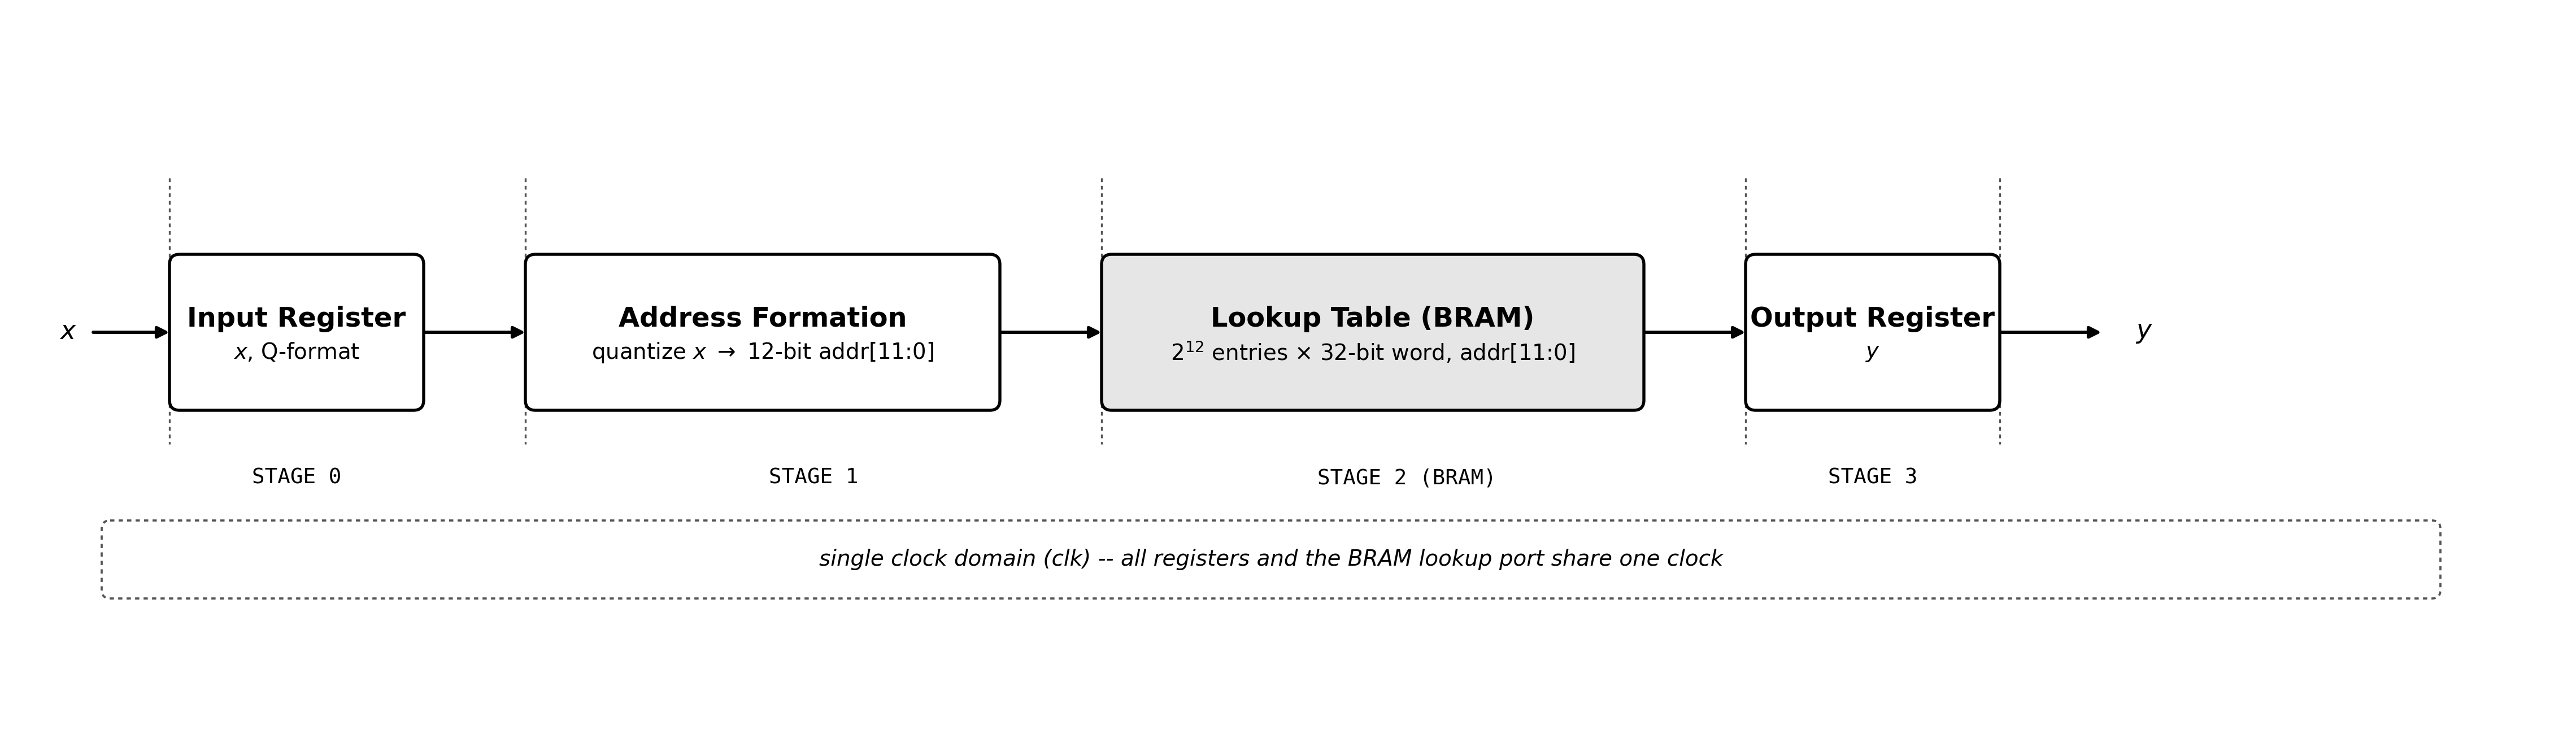
\includegraphics[width=\linewidth]{figures/pipeline1.png}
\caption{Direct LUT reciprocal architecture.}
\Description{Left-to-right block diagram with four stages in series: an input register, an address-formation block that keeps the top 12 bits of the input, a single block RAM read, and an output register. No multiplier or adder appears anywhere in the path. The pipeline is 5 cycles deep in Q8.24 and 3 cycles deep in Q16.16.}
\label{fig:directlut}
\end{figure}

\subsection{LUT-Interpolation}
\label{sec:arch-interp}

The interpolation architecture reduces the seed table to 11 address bits and adds a linear interpolation stage per Eq.~(\ref{eq:interp}). In addition to the coarser reciprocal-value table, a second table (or a second field of the same table row) stores the local slope $S[i]$ between the current breakpoint and the next. The datapath (Fig.~\ref{fig:lutinterp}) computes the fractional offset $(x - x_i)$ from the low-order bits of the input not consumed by the address, multiplies this offset by the stored slope, and adds the product to the base table value $L[i]$. This requires one multiplier and one adder beyond the Direct LUT datapath, which is reflected in the non-zero DSP and substantially higher slice LUT/FF utilization reported in Table~\ref{tab:resources}, but yields roughly an order-of-magnitude improvement in maximum relative error relative to the Direct LUT architecture (9.4$\times$ in Q8.24 and 10.4$\times$ in Q16.16) even though its address is only one bit narrower (11 versus 12 bits).

\begin{figure}[H]
\centering
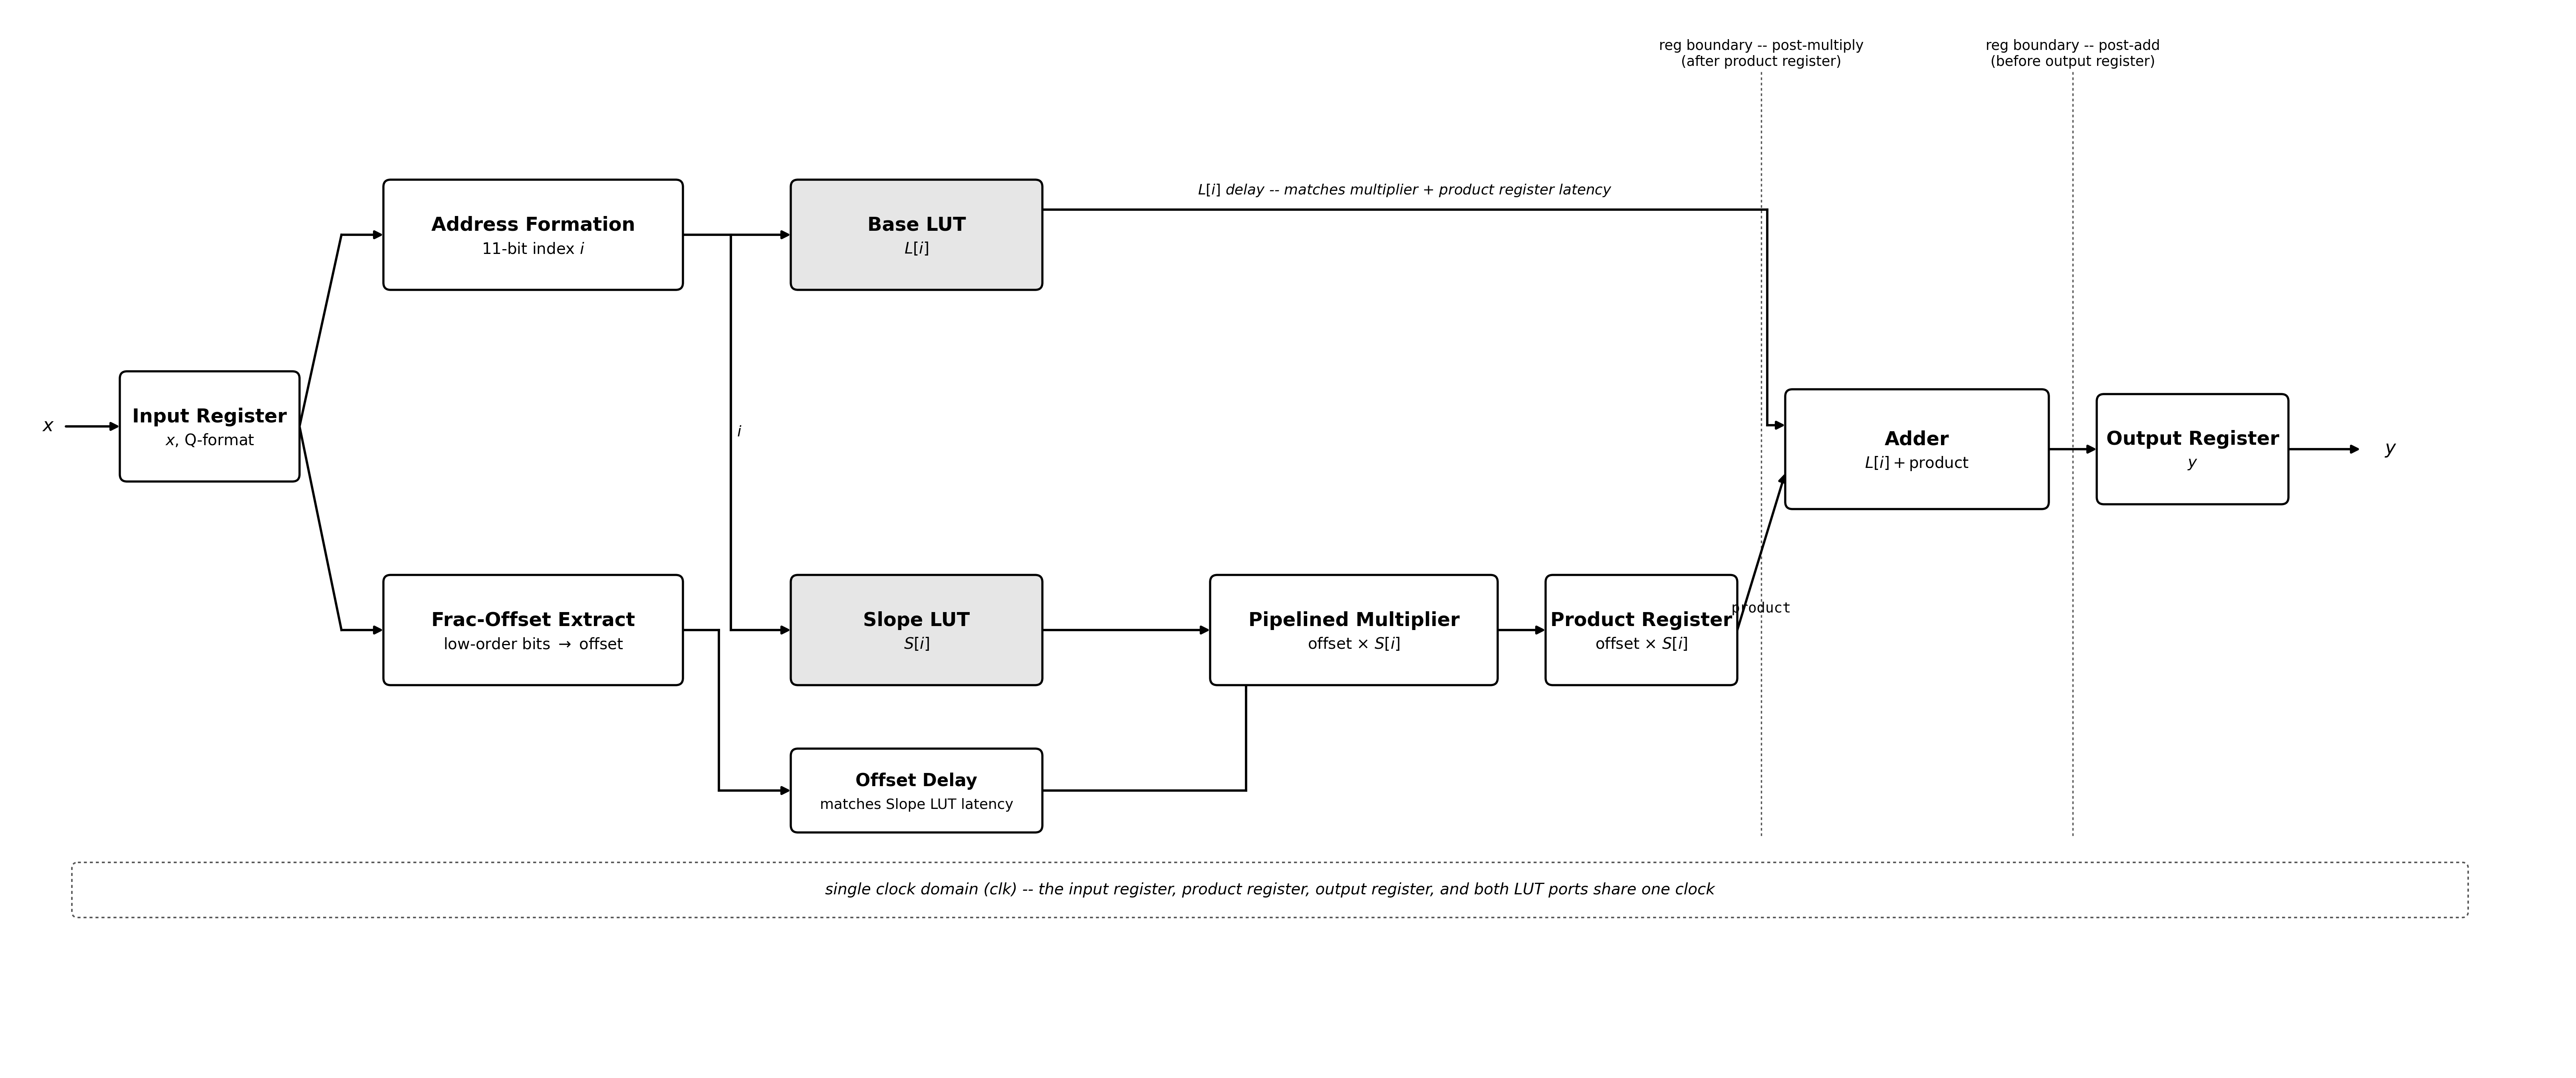
\includegraphics[width=\linewidth]{figures/pipeline2.png}
\caption{LUT-Interpolation reciprocal architecture.}
\Description{Block diagram in which an 11-bit address reads a base-value table and a slope table in parallel. The remaining low-order input bits form the fractional offset, which enters a single multiplier together with the slope. The product is added to the base value in one adder before the output register. The complete pipeline is 16 cycles deep in both formats.}
\label{fig:lutinterp}
\end{figure}

\subsection{Newton-Raphson}
\label{sec:arch-nr}

The Newton-Raphson architecture computes an 8-bit-address seed estimate $y_0$ from a coarse BRAM lookup table and applies two Newton-Raphson refinement iterations using Eq.~(\ref{eq:nr}). The first iteration computes $y_1 = y_0(2 - xy_0)$, while the second computes $y_2 = y_1(2 - xy_1)$, with $y_2$ used as the final reciprocal estimate. Each iteration consists of two sequential $32\times32$ fixed-point multiplications with a subtraction from the constant 2 between them, giving four sequential multiplications and two subtraction operations per reciprocal estimate. The datapath is implemented using the deeply pipelined \texttt{pipelined\_mult32x32\_signed} multiplier and the \texttt{reciprocal\_nr\_q8\_24} iteration-control structure. Because the four multiplications form a serial dependency chain across the two refinement iterations, the Newton-Raphson architecture has the deepest multiplier pipeline among the evaluated architectures, resulting in a 69-cycle pipeline at the target clock (Fig.~\ref{fig:newtonraphson}).

\begin{figure}[H]
\centering
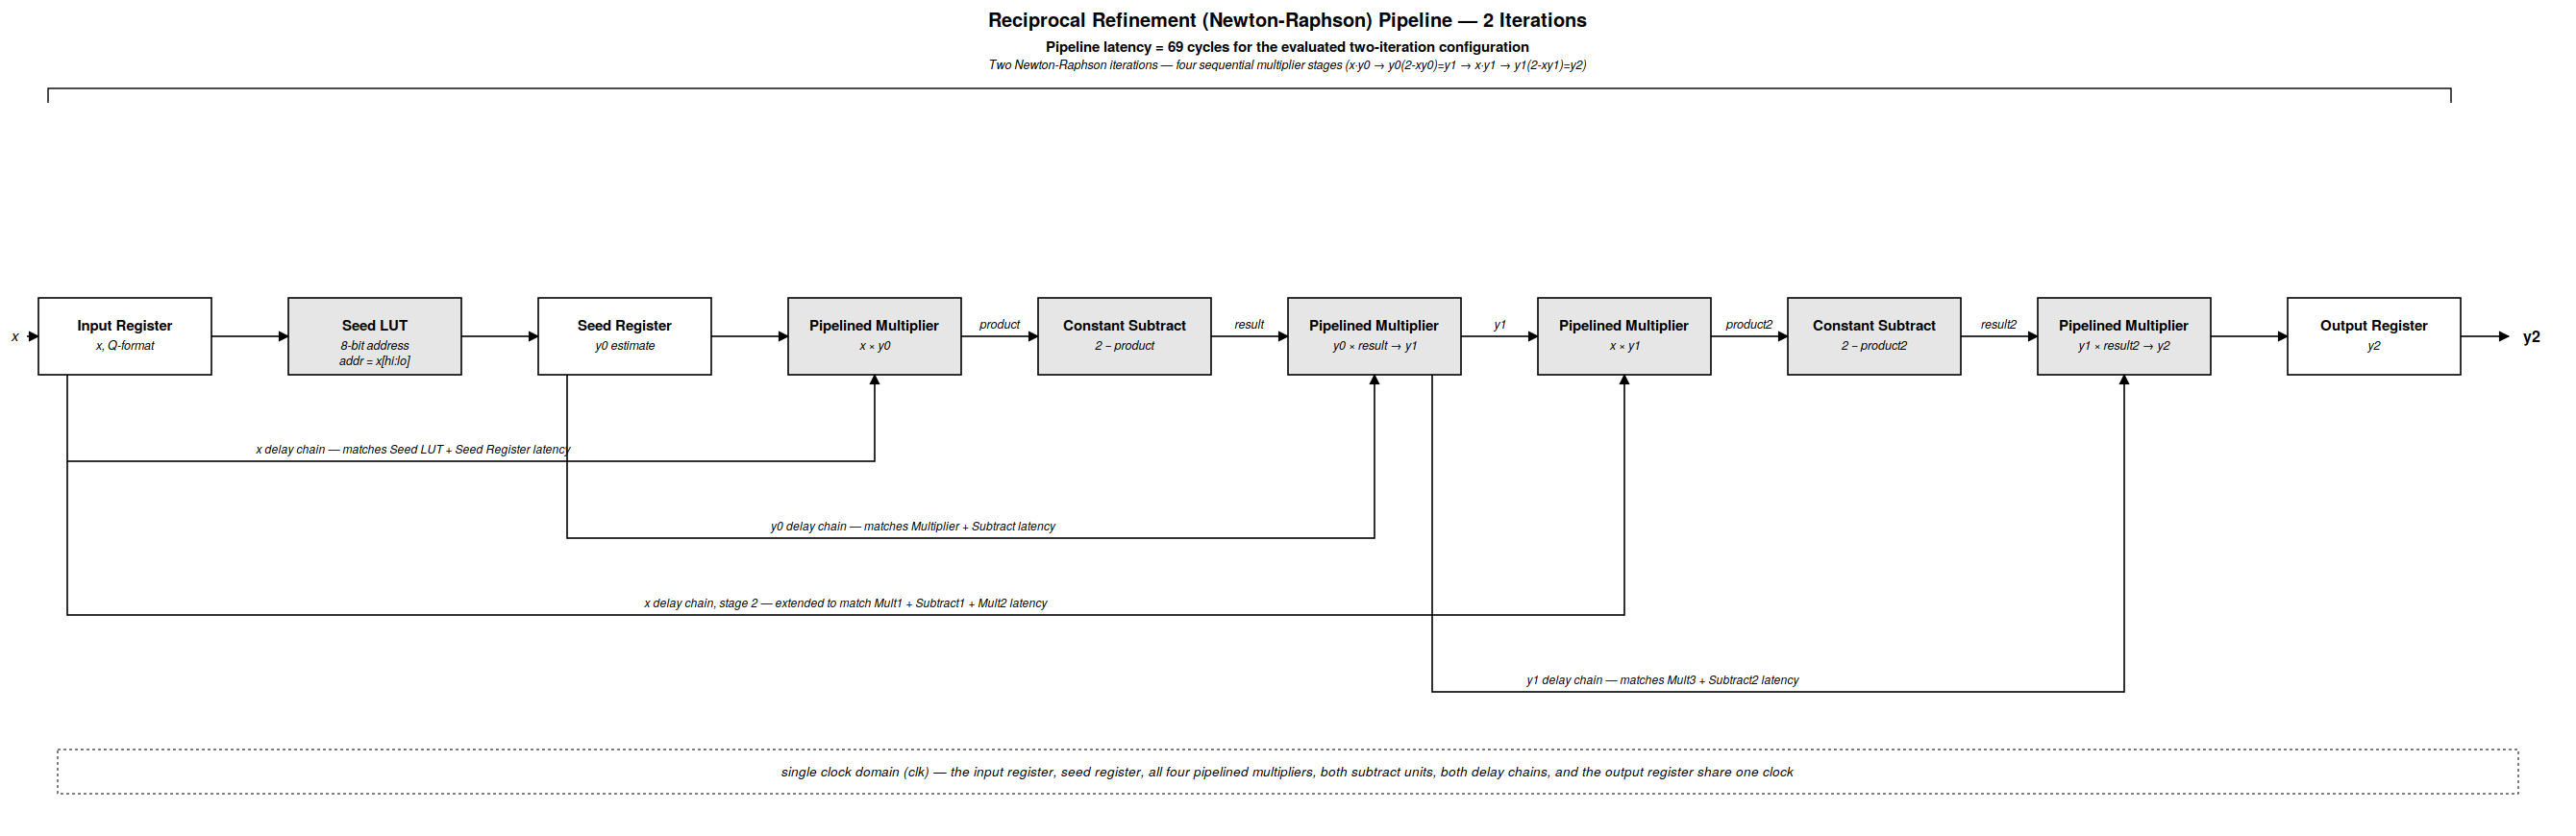
\includegraphics[width=\linewidth]{figures/pipeline3.png}
\caption{Newton-Raphson reciprocal architecture.}
\Description{Block diagram of an 8-bit-address seed table followed by two identical refinement blocks in series. Each block multiplies the input by the current estimate, subtracts the result from the constant 2, and multiplies again by the current estimate. The four multiplications therefore form one serial chain, giving a 69-cycle pipeline.}
\label{fig:newtonraphson}
\end{figure}

\subsection{Goldschmidt}
\label{sec:arch-gs}

The Goldschmidt architecture uses the same 8-bit-address seed table as Newton-Raphson but restructures the refinement as the mutually recursive numerator/denominator update of Eqs.~(\ref{eq:gold_init}) and~(\ref{eq:gold_update}). The two multiplications $F_i \times N_i$ and $F_i \times D_i$ within a given iteration do not depend on one another and can therefore be scheduled in parallel across two multiplier instances, rather than sequentially through one multiplier instance as in Newton-Raphson. This parallelism shortens the achievable pipeline depth per iteration (54 cycles versus 69 for Newton-Raphson at the same clock target) at the cost of a second parallel multiplier datapath. The final reciprocal estimate is read from the $N_i$ register once the iteration count is reached (Fig.~\ref{fig:goldschmidt}).

\begin{figure}[H]
\centering
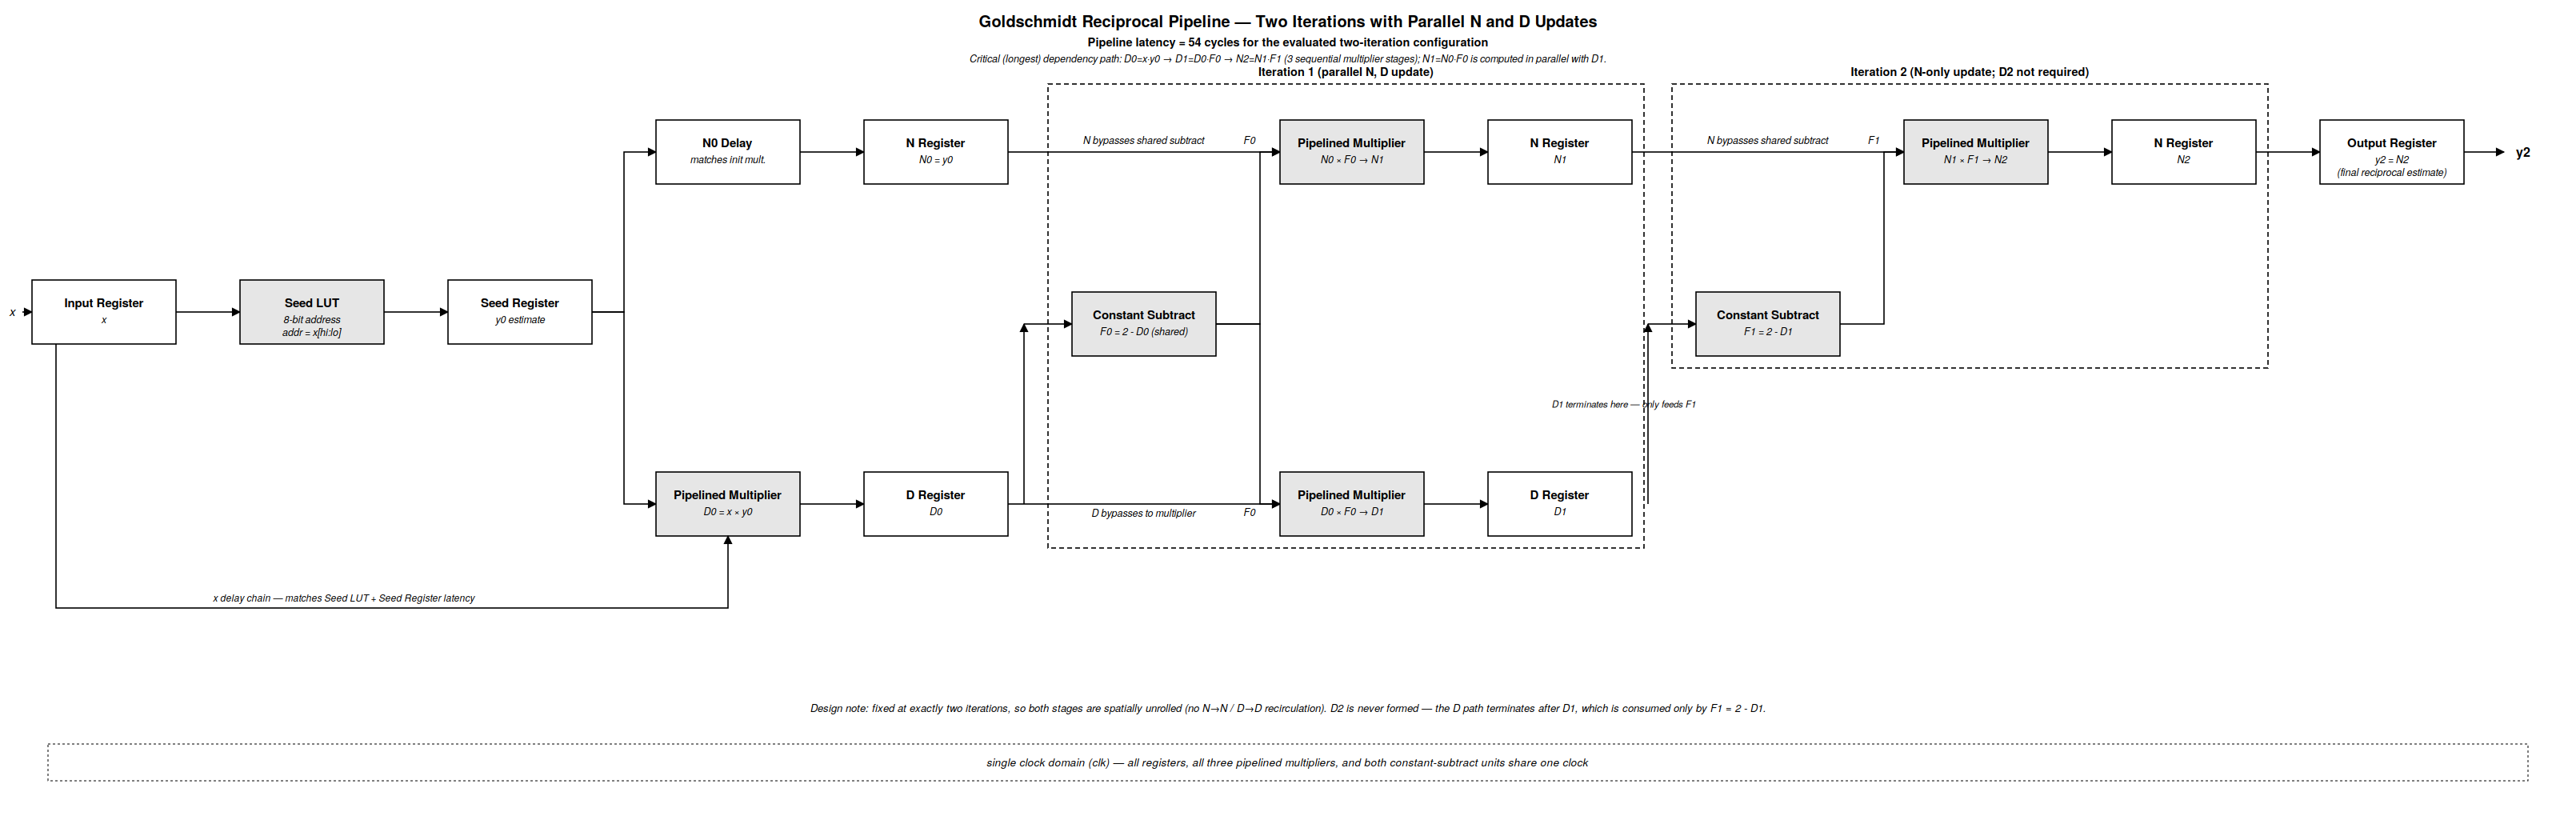
\includegraphics[width=\linewidth]{figures/pipeline4.png}
\caption{Goldschmidt reciprocal architecture.}
\Description{Block diagram in which the seed table output forms the initial numerator and, after one multiplication by the input, the initial denominator. Two refinement iterations follow. In each, a correction factor is computed from the denominator and two multipliers update the numerator and denominator side by side. The final result is taken from the numerator register after the second iteration. The pipeline is 54 cycles deep.}
\label{fig:goldschmidt}
\end{figure}

\subsection{Hybrid LUT-Interpolation/Newton-Raphson}
\label{sec:arch-hybrid}

The Hybrid architecture (module name \texttt{reciprocal\_hybrid9\_1nr\_q8\_24} in the Q8.24 configuration) combines LUT-Interpolation with a single Newton-Raphson refinement stage. It first generates an interpolated reciprocal estimate using a 9-bit-address LUT-and-interpolation stage, providing a finer initial approximation than the 8-bit-address seed LUTs used by the standalone iterative architectures. The interpolated estimate is then refined using a single Newton-Raphson iteration of Eq.~(\ref{eq:nr}), rather than applying the iteration directly to a coarse LUT output. Since the interpolated estimate has a smaller initial error, the refinement can achieve substantially higher accuracy while avoiding the deeper pipeline required by the standalone Newton-Raphson architecture. The complete hybrid design (Fig.~\ref{fig:hybrid}) comprises four constituent modules: \texttt{reciprocal\_interp9\_q8\_24} for the interpolation seed stage, \texttt{mult32x32\_pipe\_q8\_24} for the shared pipelined multiplier, \texttt{nr\_iterate\_q8\_24} for the single-iteration refinement, and \texttt{reciprocal\_hybrid9\_1nr\_q8\_24} as the top-level integration wrapper.

\begin{figure}[H]
\centering
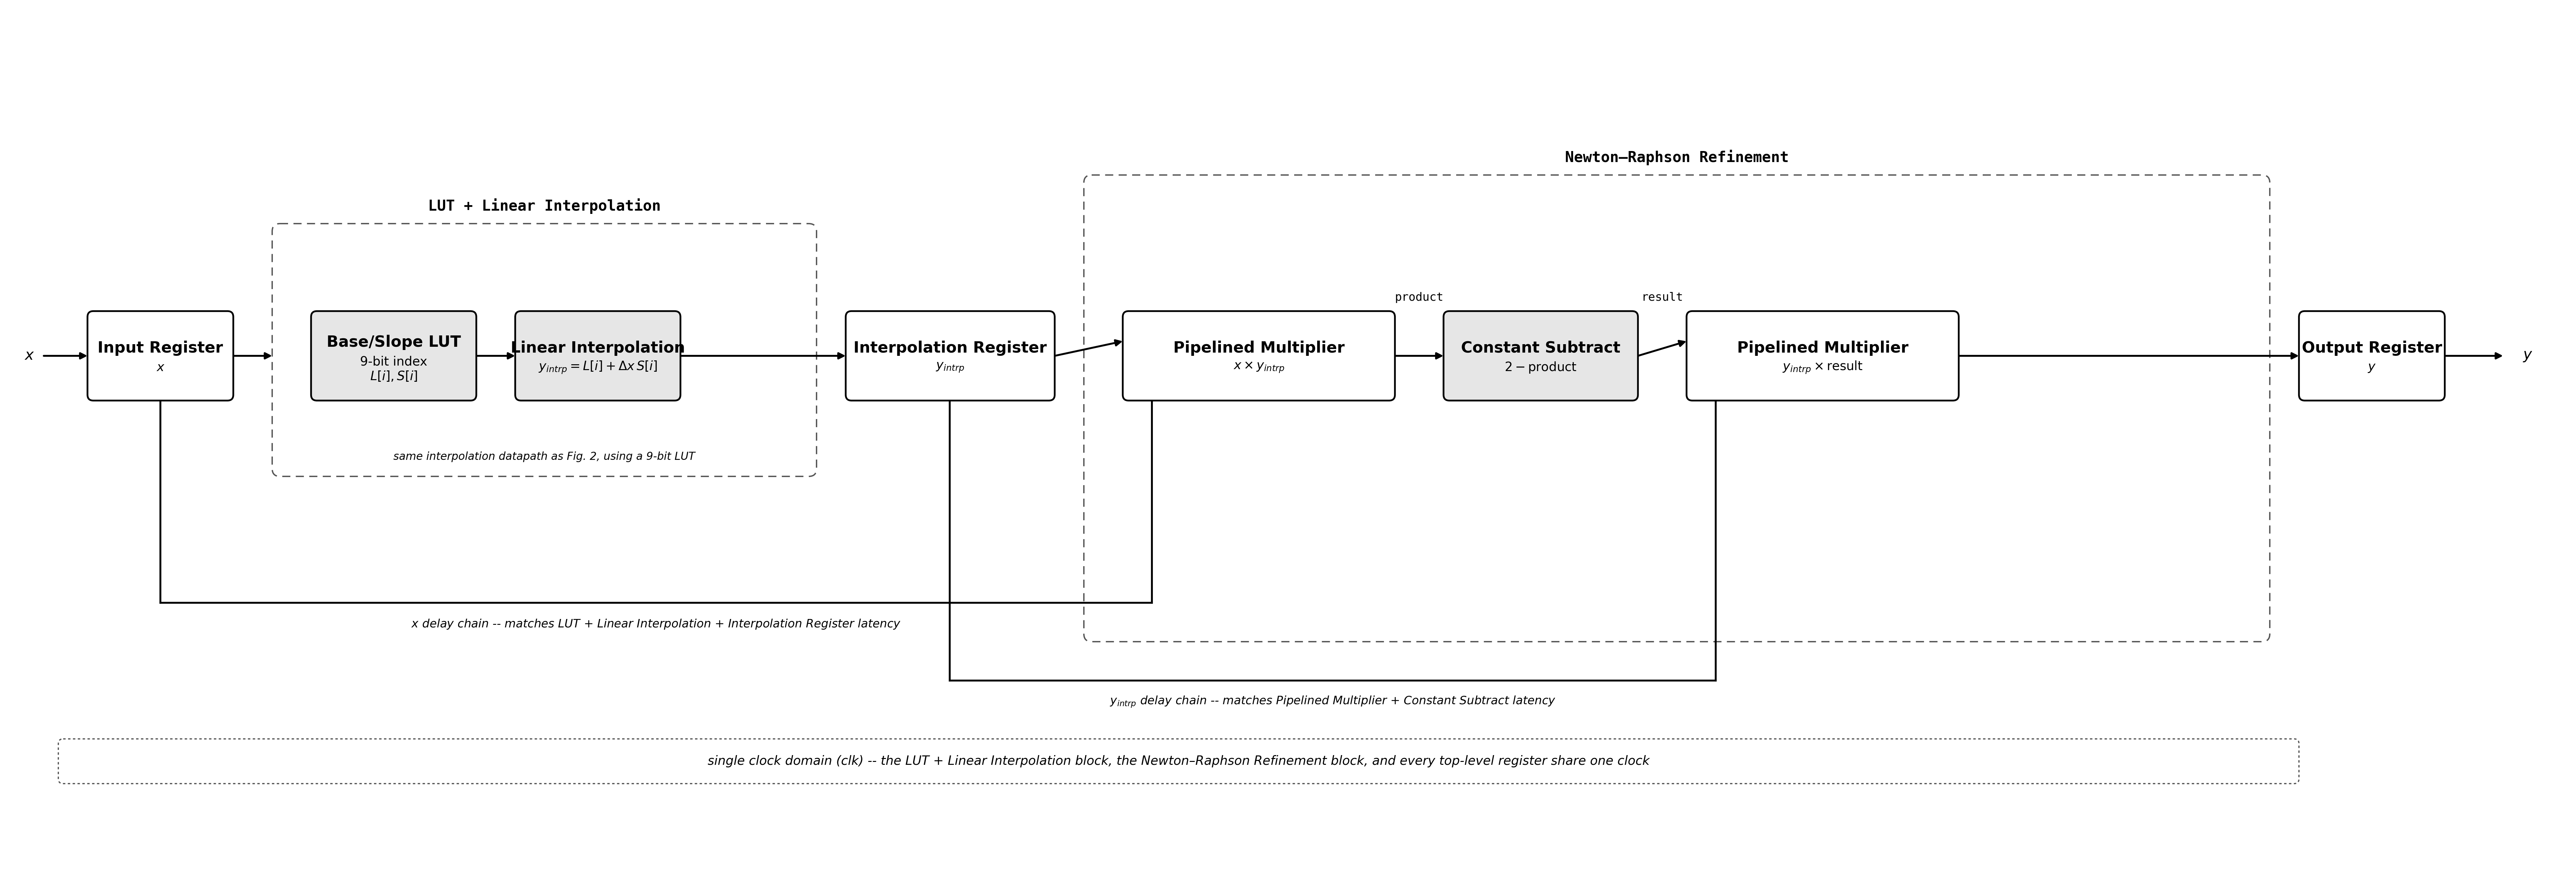
\includegraphics[width=\linewidth]{figures/pipeline5.png}
\caption{Hybrid LUT-Interpolation/Newton-Raphson reciprocal architecture.}
\Description{Block diagram of a 9-bit-address interpolation stage, built from a table read, one multiplication and one addition, whose output feeds a single Newton-Raphson iteration of two multiplications and one subtraction. The multiplications share one pipelined multiplier module. The whole pipeline is 40 cycles deep.}
\label{fig:hybrid}
\end{figure}

\subsection{Common Hardware Configuration}
\label{sec:common-hw}

All five architectures share a common set of implementation conventions to keep the comparison controlled. Each architecture is implemented as a fully pipelined datapath with registers inserted at every internal arithmetic stage boundary, so that after the pipeline fill latency, one new result is produced every clock cycle; this is what allows the Max Throughput (Mops/s) figures reported in Section~\ref{sec:results} to equal the achieved $F_{\max}$ directly, rather than a fraction of it. All five architectures were synthesized and implemented for a Xilinx Artix-7 device (Nexys A7-100T development board \cite{DigilentNexysA7}, part xc7a100tcsg324-1) using the Xilinx Vivado design suite (2025.2.1), with out-of-context synthesis and full place-and-route implementation performed independently for each architecture/format combination at its own clock target (2.58~ns for the four 387.6~MHz-targeted architectures, 3.333~ns for the Hybrid architecture's 300~MHz target, per Table~\ref{tab:designparams}). The clock targets are therefore architecture-specific rather than identical: the Hybrid architecture was implemented against a less aggressive target than the other four, selected according to the timing requirements of its datapath (an interpolation stage followed by a Newton-Raphson refinement). Its latency and $F_{\max}$ figures should accordingly be read against that constraint rather than as results obtained under an identical clock requirement. The pipelined multipliers used throughout the iterative and hybrid datapaths map onto the device's DSP48E1 slices, each of which integrates a pre-adder, a $25 \times 18$ multiplier, and a configurable adder/accumulator with internal cascade paths \cite{XilinxUG479}; the DSP utilization figures reported in Table~\ref{tab:resources} are counted in units of these slices. During implementation, multiple Vivado synthesis and implementation optimization strategies were used, including \texttt{AggressiveExplore}, \texttt{ExtraTimingOpt}, and \texttt{Explore} strategies, together with timing-oriented implementation directives, to obtain the best achievable timing under the stated architectural constraints. The same optimization methodology was applied across the architectures rather than relying on a single default implementation strategy. Two architecture/format combinations (Newton-Raphson and Goldschmidt) additionally required attribute-level intervention during physical synthesis (\texttt{dont\_touch} constraints on selected register stages) to prevent Vivado's retiming optimizer from merging or removing intended pipeline register boundaries; this is discussed further in Section~\ref{sec:timing-closure}.

\subsection{Algorithmic Complexity}

Table~\ref{tab:opcount} summarizes each architecture's datapath in terms of primitive operation counts (multiplications, additions/subtractions, and memory reads) per complete reciprocal estimate. Direct LUT requires a single memory read and no arithmetic, while LUT-Interpolation adds one multiply and one add to the two table reads used for the stored breakpoint value and slope. Newton-Raphson performs two refinement iterations, with each iteration requiring two sequential multiplications and one subtraction, giving four multiplications and two subtractions per reciprocal estimate. Goldschmidt also performs two refinement iterations; its initialization requires one multiplication to form $D_0 = xy_0$, the first refinement computes $N_1 = N_0 F_0$ and $D_1 = D_0 F_0$ using two parallel multiplications, and the second refinement computes the final $N_2 = N_1 F_1$, giving four multiplications and two subtractions in total. The Hybrid architecture combines one interpolation stage with a single Newton-Raphson refinement, resulting in three multiplications and two additions/subtractions per reciprocal estimate. The parallel organization of Goldschmidt reduces sequential multiplier depth relative to Newton-Raphson without reducing the total arithmetic operation count.

\begin{table}[H]
\caption{Algorithmic Operation Count per Reciprocal Estimate}
\label{tab:opcount}
\begin{tabular}{@{}lcccl@{}}
\toprule
\textbf{Architecture} & \textbf{Mult.} & \textbf{Add/Sub} & \textbf{Mem. Reads} & \textbf{Seed Table Address} \\
\midrule
Direct LUT & 0 & 0 & 1 & 12-bit address \\
LUT-Interpolation & 1 & 1 & 2 & 11-bit address \\
Newton-Raphson & 4 & 2 & 1 & 8-bit address \\
Goldschmidt & 4 & 2 & 1 & 8-bit address \\
Hybrid & 3 & 2 & 2 & 9-bit address \\
\bottomrule
\end{tabular}
\end{table}

\section{Experimental Methodology}
\label{sec:methodology}

\subsection{Verification Methodology}
\label{sec:verification}

Functional correctness and numerical accuracy for all five architectures, in both fixed-point formats, were verified against a common double-precision software reference model computing $1/x$ directly. Each architecture was exercised over one million verification vectors swept uniformly across the input domain $x \in [0.5, 2.5]$, with the bit-accurate RTL simulation output compared against the reference value at matching precision. This uniform sweep is a dense sample of the input domain rather than an enumeration of every representable input. For each output sample, the signed error is defined in least-significant-bit (LSB) units as
\begin{equation}
e[n] = y_{hw}[n] - \mathrm{round}\!\left(y_{ref}[n]\, 2^F\right)
\label{eq:lsberror}
\end{equation}
Here, $y_{hw}[n]$ is the hardware/RTL output represented as a raw integer in the device's Q-format, $y_{ref}[n]$ is the double-precision reference reciprocal, and $F$ is the number of fractional bits for the format under test. For relative-error calculation, the hardware output is converted to real-valued form as $y_{hw,real}[n] = y_{hw}[n]\, 2^{-F}$. The maximum relative error is then defined as
\begin{equation}
E_{\max,rel} = \max_n \left( \frac{|y_{hw,real}[n] - y_{ref}[n]|}{|y_{ref}[n]|} \right) \times 100\%
\label{eq:maxrelerror}
\end{equation}
Maximum relative error is used as the primary accuracy metric in the Pareto analysis of Section~\ref{sec:pareto} because, unlike a raw LSB count, it is directly comparable across the two evaluated fixed-point formats: one LSB of Q8.24 ($2^{-24}$) and one LSB of Q16.16 ($2^{-16}$) represent different absolute quantities, so an LSB-based error metric cannot be used to rank accuracy across formats without first normalizing by format resolution, which the relative-error metric does implicitly. All pipelined architectures exhibit a warm-up transient during the first $N_{cycles}$ output samples, corresponding to the pipeline fill period before the first valid result reaches the output register; these initial samples are excluded from all summary error statistics and are visualized explicitly in Section~\ref{sec:accuracy} (pipeline warm-up plots).

\subsection{Timing Closure}
\label{sec:timing-closure}

Timing closure was the most implementation-intensive part of this work, particularly for the two full iterative architectures (Newton-Raphson and Goldschmidt), each of which required multiple revision cycles to close timing at their 387.6~MHz target on the Artix-7 fabric. Several recurring classes of timing violation were encountered and resolved across the iterative architectures' revision history. First, wide fixed-point adders synthesized as single-stage CARRY4 chains repeatedly failed to meet the target period and had to be manually split across pipeline stage boundaries (e.g., separating a cross-term adder from the final high-order sum in the pipelined multiplier). Second, Vivado's register-merge retiming optimization was found to silently undo manually inserted pipeline splits by merging what were intended as two distinct pipeline stages back into one combinational block. Register retiming is, in general, a valuable transformation that moves registers across combinational logic to balance path delays without changing observable circuit behavior \cite{LeisersonSaxe91}, and is applied productively to FPGA pipelines in techniques such as C-slow retiming \cite{WeaverMarkovskiyPatelWawrzynek03}; the difficulty encountered here was that automatic retiming, applied uniformly, merged register boundaries the design deliberately relied on as physical pipeline-stage markers. This was resolved by applying \texttt{dont\_touch} (and, in one case, a synthesis-level \texttt{keep}) attributes to the registers marking the intended stage boundary, since a \texttt{shreg\_extract="no"} attribute alone was found to be insufficient to prevent this class of retiming. Third, DSP48E1 cascade inference was found to occasionally fuse an intended register boundary directly into the DSP slice's internal C-port cascade path, bypassing the pipeline register the designer intended to be a hard stage boundary; this required explicit attribute-level or structural intervention to restore the intended pipeline stage count.

A related correctness (rather than timing) issue surfaced during this process: a one-cycle discrepancy in the reported latency of a signed dedicated-adder submodule (\texttt{dsp\_add18x18\_signed}) caused a systematic, low-probability functional error that was only caught by the full one-million-vector verification sweep described in Section~\ref{sec:verification} rather than by smaller directed test sets, underscoring the value of dense-sweep verification for pipelined fixed-point arithmetic where an off-by-one-cycle latency bug can silently corrupt only a small fraction of the output space. Once identified, the fix consisted of correcting the tracked \texttt{MULT\_LATENCY} parameter used to align data with its corresponding valid/control signal through the pipeline, together with a corrected operand-port assignment inside the same submodule.

\subsection{Power Estimation and Energy Derivation}

Dynamic and static power values reported in Section~\ref{sec:power} were obtained from Vivado's post-implementation power analysis for each architecture/format combination. These values are tool-based estimates rather than direct measurements of board-level power consumption, and they do not rely on a validated switching-activity trace from the verification sweep. Because every evaluated architecture is fully pipelined to produce one valid output per clock cycle once its pipeline is filled, the sustained throughput of each architecture in operations per second is equal to its achieved $F_{\max}$. Energy per operation was subsequently derived from the reported total power and this throughput as
\begin{equation}
E_{op} = \frac{P_{total}}{F_{\max}}
\label{eq:energyop}
\end{equation}
This relationship treats the estimated total power as corresponding to operation at the achieved $F_{\max}$. It reproduces the reported Energy/op values in Table~\ref{tab:power} for all ten architecture/format combinations to within rounding, and it is the basis of every Energy/op figure used in the Pareto analysis of Section~\ref{sec:pareto}. Reported latency in nanoseconds (Table~\ref{tab:timing}) is computed separately from the achieved $F_{\max}$, as the product of the architecture's fixed pipeline depth in clock cycles and its target clock period:
\begin{equation}
L_{ns} = N_{cycles} \times T_{target}
\label{eq:latency}
\end{equation}
using the target clock period from Table~\ref{tab:designparams} rather than the achieved period, so that latency reflects the architecture's designed pipeline depth independent of any timing margin achieved beyond the target frequency.

\section{Experimental Results}
\label{sec:results}

This section presents post-implementation results across resource utilization, timing and latency, numerical accuracy, and power/energy for all five architectures in both evaluated fixed-point formats, followed by a direct cross-format comparison in Section~\ref{sec:crossformat}. A consolidated summary of all metrics is given in Section~\ref{sec:consolidated}.

\subsection{Resource Utilization}

Table~\ref{tab:resources} and Fig.~\ref{fig:resources} report post-implementation resource utilization for all ten architecture/format combinations. The Direct LUT architecture consumes negligible slice LUT and flip-flop resources but requires \textbf{3.5 BRAMs in Q8.24, tied with LUT-Interpolation for the largest BRAM allocation among the evaluated configurations}, since it must store a full-precision reciprocal value at every one of its 4096 addressable entries. The two full iterative architectures (Newton-Raphson and Goldschmidt) show substantially higher slice LUT and flip-flop utilization than the table-based architectures, roughly 5 to 7 times that of LUT-Interpolation, reflecting their pipelined multiplier datapaths, and both consume the maximum 20 DSP48E1 slices allocated to the pipelined multiplier chains. The Hybrid architecture sits between the interpolation and full-iterative architectures on slice LUT/FF count, consistent with its interpolated seed followed by a single Newton-Raphson refinement iteration, while requiring roughly half the DSP count of the full iterative architectures (9 versus 20).

\begin{table}[H]
\caption{Post-Implementation Resource Utilization}
\label{tab:resources}
\begin{tabular}{@{}llrrrrr@{}}
\toprule
\textbf{Architecture} & \textbf{Format} & \textbf{Slice LUT} & \textbf{Slice LUT\%} & \textbf{FF} & \textbf{DSP} & \textbf{BRAM} \\
\midrule
Direct LUT & Q8.24 & 19 & 0.03\% & 84 & 0 & 3.5 \\
Direct LUT & Q16.16 & 2 & 0.003\% & 51 & 0 & 2.5 \\
LUT-Interpolation & Q8.24 & 159 & 0.25\% & 685 & 1 & 3.5 \\
LUT-Interpolation & Q16.16 & 119 & 0.19\% & 647 & 1 & 2.0 \\
Newton-Raphson & Q8.24 & 966 & 1.52\% & 3612 & 20 & 0.5 \\
Newton-Raphson & Q16.16 & 849 & 1.34\% & 3340 & 20 & 0.5 \\
Goldschmidt & Q8.24 & 846 & 1.33\% & 3656 & 20 & 0.5 \\
Goldschmidt & Q16.16 & 722 & 1.14\% & 3385 & 20 & 0.5 \\
Hybrid & Q8.24 & 768 & 1.21\% & 2626 & 9 & 1.0 \\
Hybrid & Q16.16 & 799 & 1.26\% & 2586 & 9 & 1.0 \\
\bottomrule
\end{tabular}
\end{table}

\begin{figure}[H]
\centering
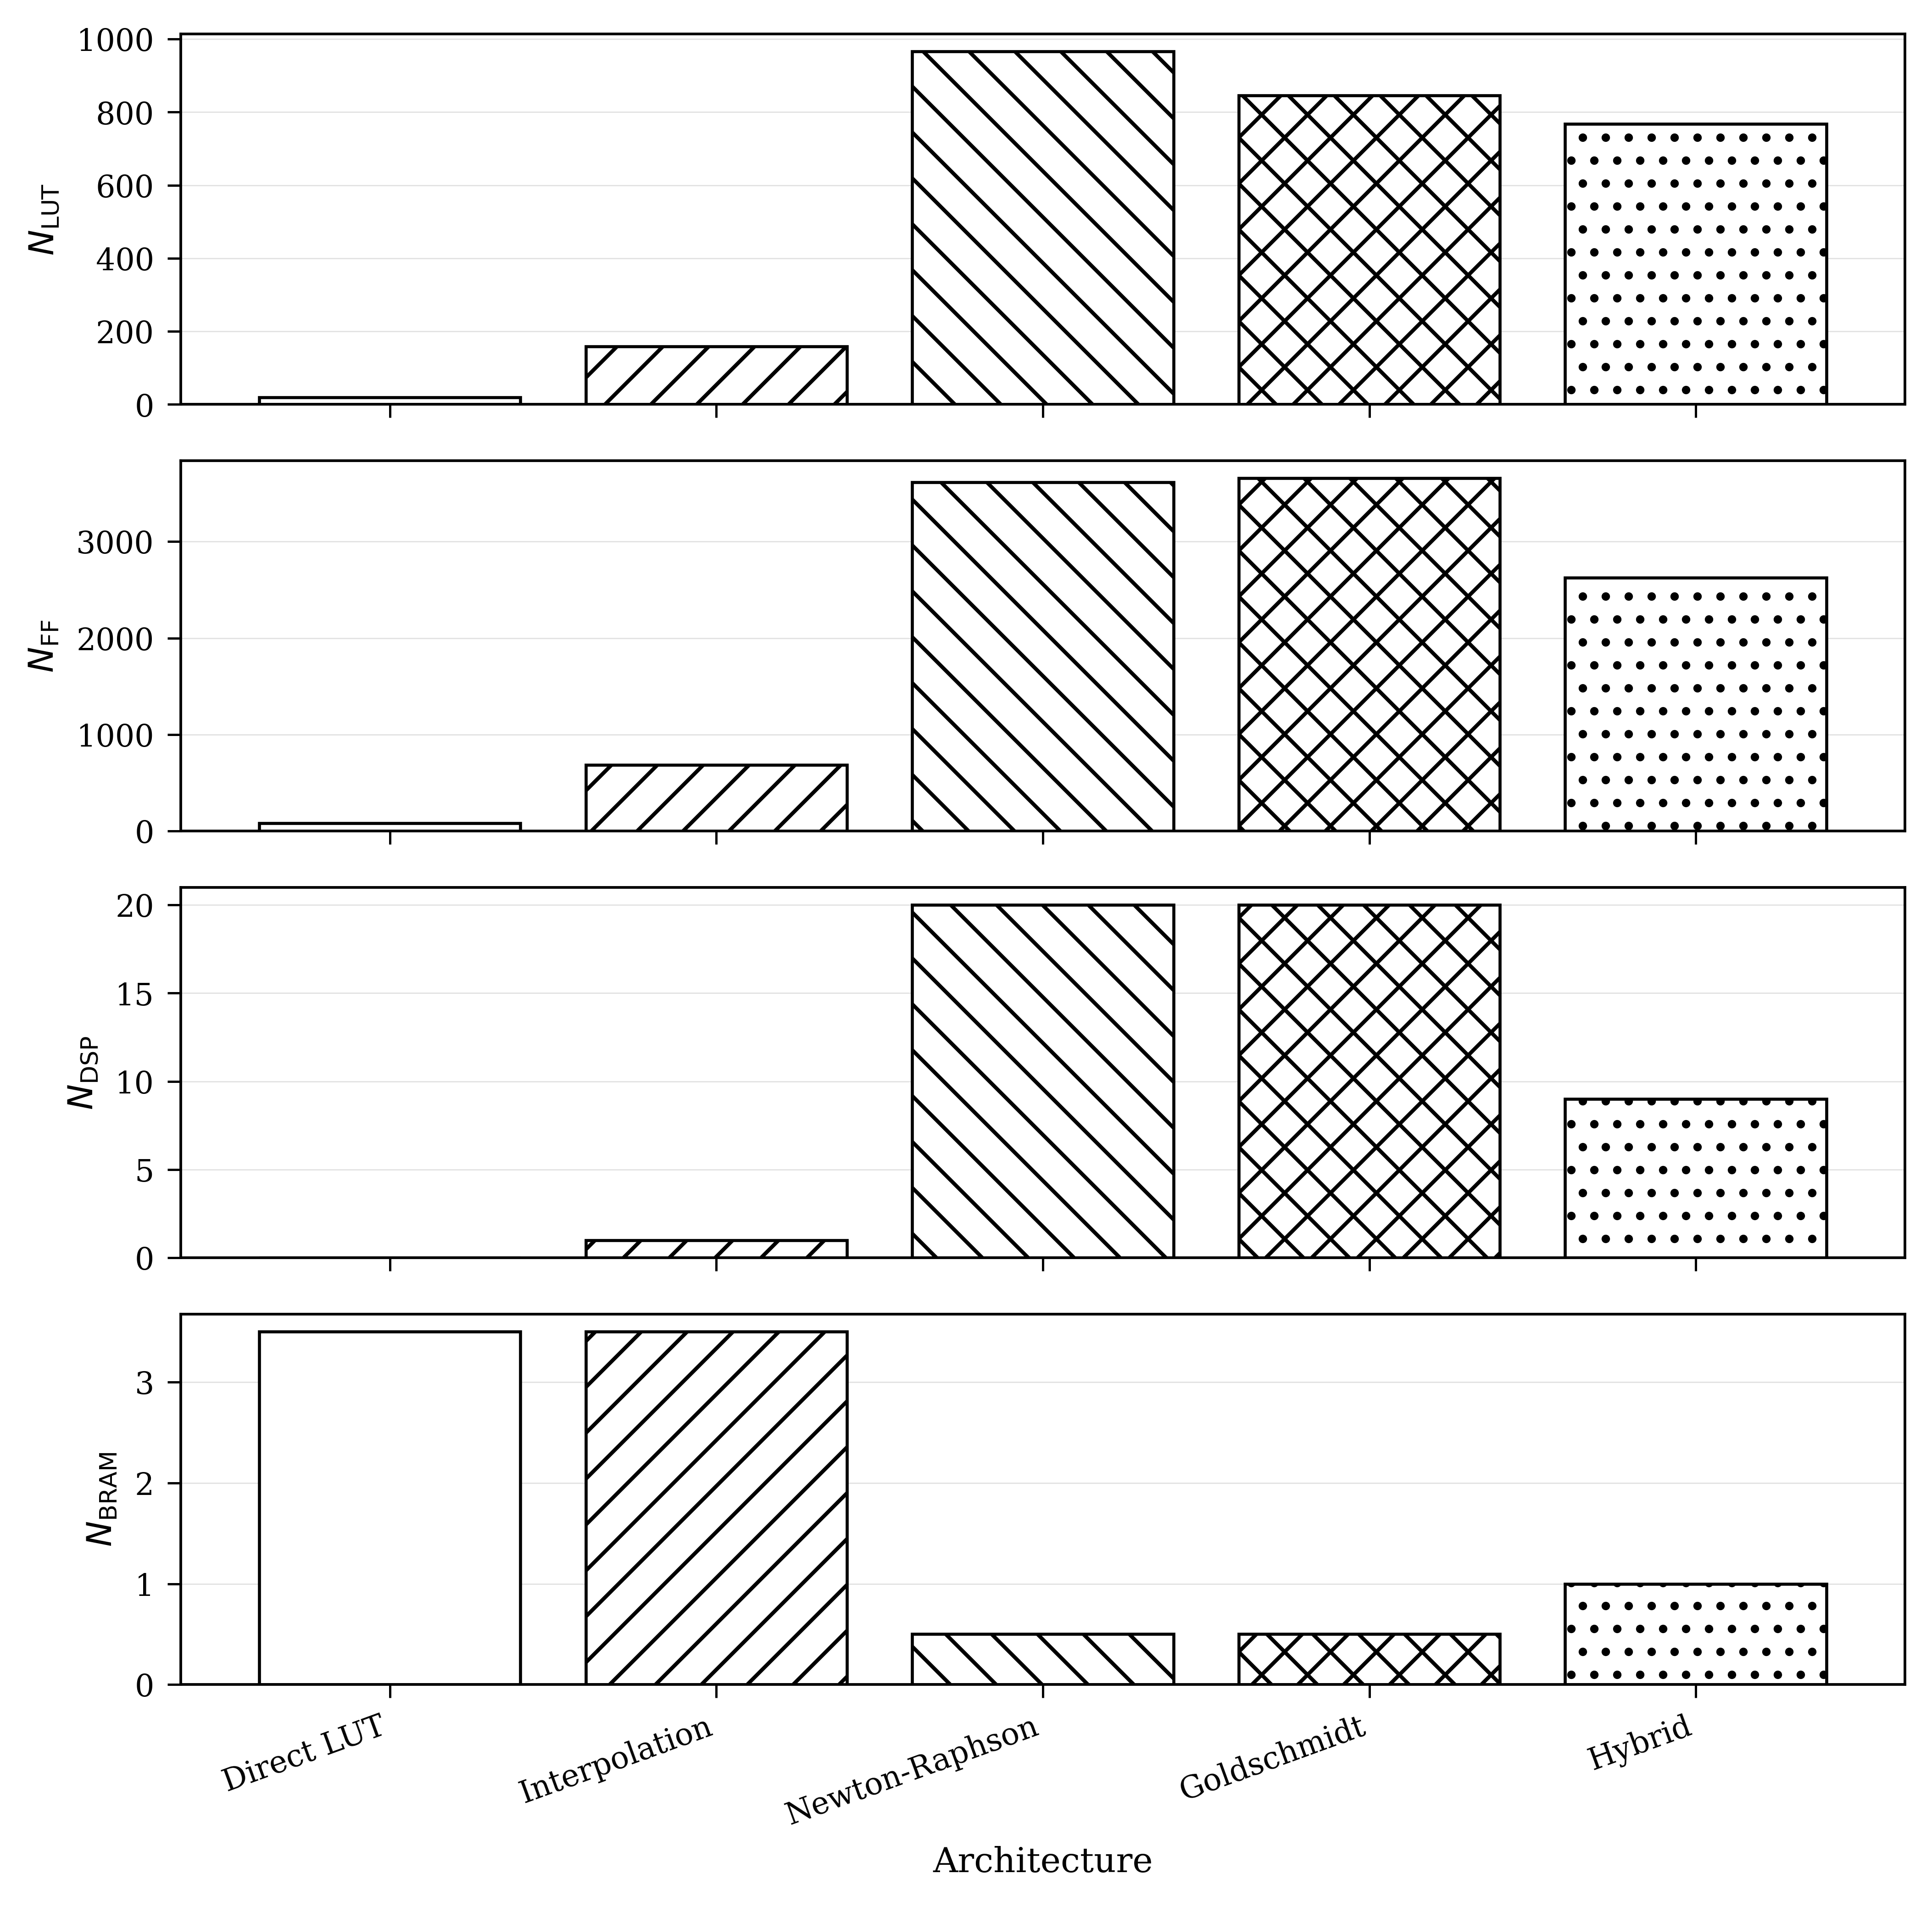
\includegraphics[width=0.49\columnwidth]{figures/q8_resource.png}
\hfill
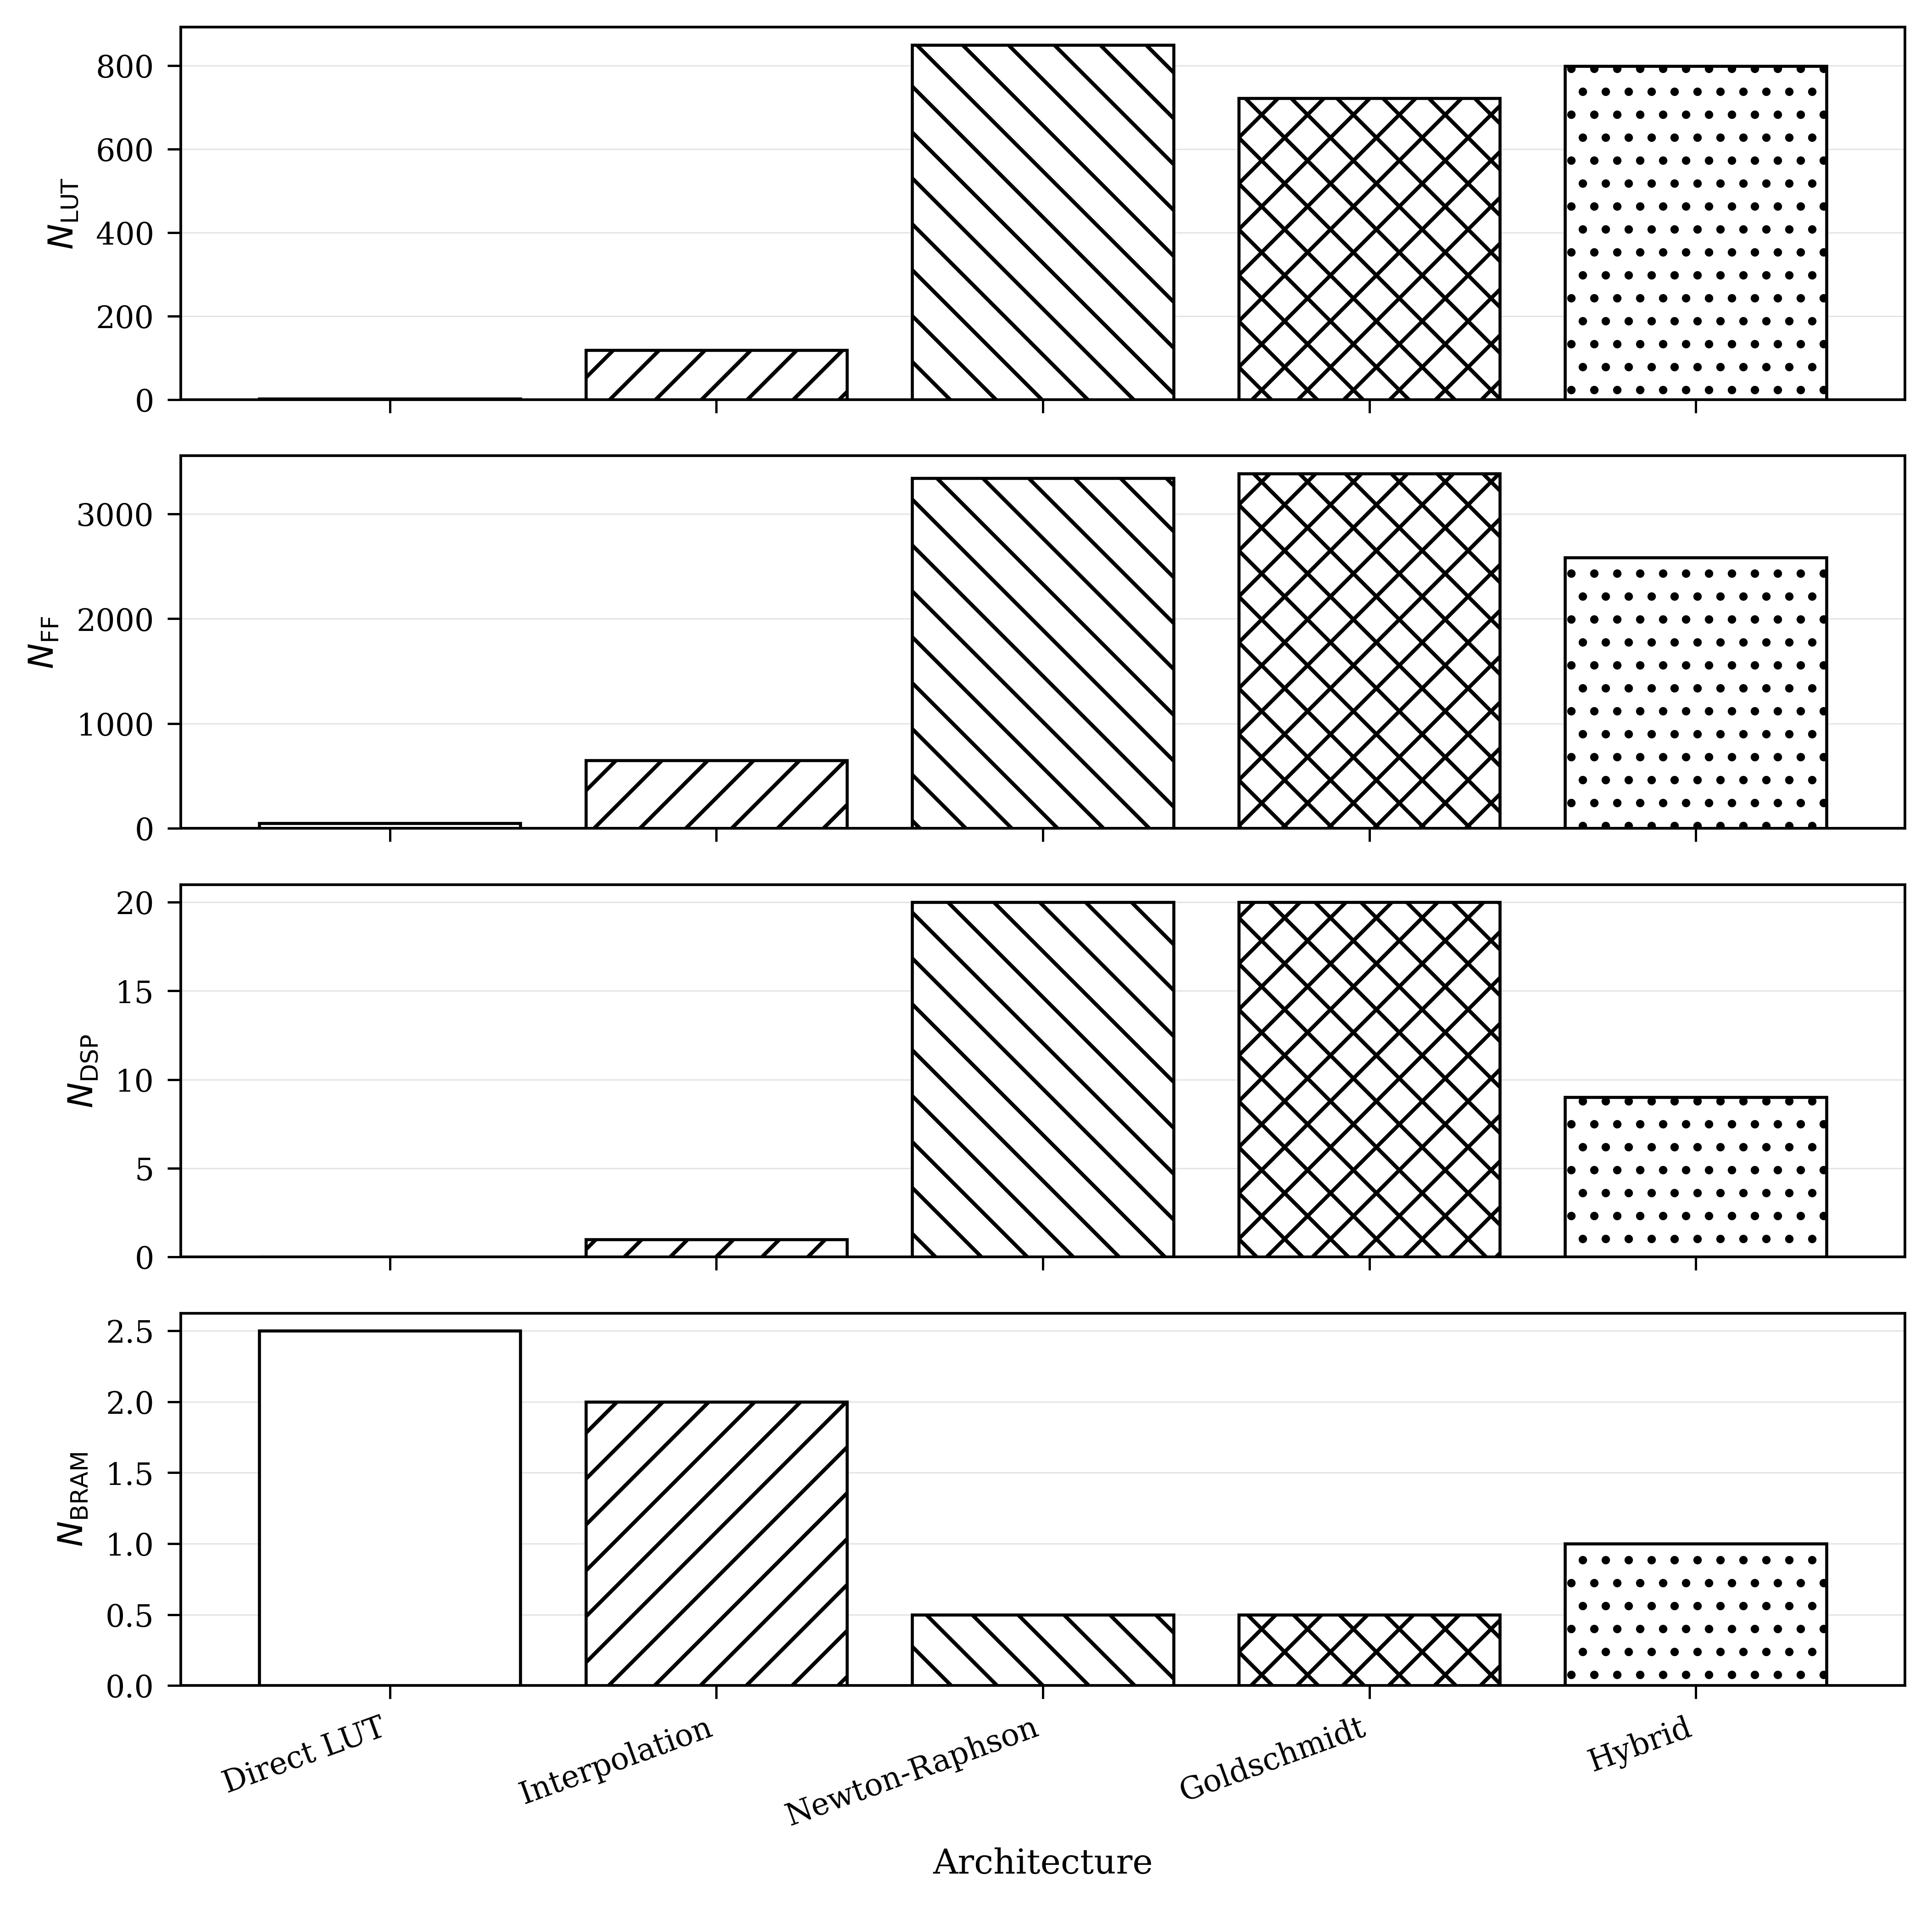
\includegraphics[width=0.49\columnwidth]{figures/q16_resource.png}

\caption{Post-implementation slice LUT, FF, DSP, and BRAM utilization (resource counts) by architecture, Q8.24 (left) and Q16.16 (right)}
\Description{Two panels of grouped bars. In both panels the Direct LUT bars for LUTs and flip-flops are close to zero, with 3.5 BRAMs in Q8.24 and 2.5 BRAMs in Q16.16. The Newton-Raphson and Goldschmidt bars are the tallest, at about 720 to 970 LUTs, 3300 to 3660 flip-flops and 20 DSP slices. The hybrid bars sit below them, at about 770 to 800 LUTs, 2590 to 2630 flip-flops, 9 DSP slices and 1 BRAM. LUT with interpolation uses 1 DSP slice and 119 to 159 LUTs.}
\label{fig:resources}
\end{figure}


\subsection{Timing and Latency}

Table~\ref{tab:timing} and Fig.~\ref{fig:summary} report the achieved maximum frequency ($F_{\max}$), worst negative slack (WNS) at the target clock period, pipeline depth, and corresponding latency calculated using Eq.~(\ref{eq:latency}). All ten architecture/format combinations achieve timing closure with positive slack at their respective target periods. The Direct LUT architecture has the shortest pipeline depth, requiring 5 cycles for Q8.24 and 3 cycles for Q16.16, resulting in the lowest absolute latency among the evaluated architectures. In contrast, the Newton-Raphson architecture requires the deepest pipeline at 69 cycles, reflecting the four sequentially dependent multiplication stages arising from its two refinement iterations, as described in Section~\ref{sec:arch-nr}. Goldschmidt reduces the pipeline depth to 54 cycles by exploiting parallelism between intermediate multiplier operations, representing an approximately 22\% reduction in pipeline depth relative to Newton-Raphson.

\begin{table}[H]
\caption{Post-Implementation Timing and Latency}
\label{tab:timing}
\begin{tabular}{@{}llrrrrr@{}}
\toprule
\textbf{Architecture} & \textbf{Format} & \textbf{$F_{\max}$ (MHz)} & \textbf{WNS (ns)} & \textbf{Latency (cyc.)} & \textbf{Latency (ns)} & \textbf{Throughput (Mops/s)} \\
\midrule
Direct LUT & Q8.24 & 392.77 & 0.034 & 5 & 12.90 & 392.77 \\
Direct LUT & Q16.16 & 519.21 & 0.654 & 3 & 7.74 & 519.21 \\
LUT-Interpolation & Q8.24 & 429.74 & 0.253 & 16 & 41.28 & 429.74 \\
LUT-Interpolation & Q16.16 & 424.45 & 0.224 & 16 & 41.28 & 424.45 \\
Newton-Raphson & Q8.24 & 399.20 & 0.075 & 69 & 178.02 & 399.20 \\
Newton-Raphson & Q16.16 & 392.62 & 0.033 & 69 & 178.02 & 392.62 \\
Goldschmidt & Q8.24 & 396.35 & 0.057 & 54 & 139.32 & 396.35 \\
Goldschmidt & Q16.16 & 394.94 & 0.048 & 54 & 139.32 & 394.94 \\
Hybrid & Q8.24 & 316.06 & 0.169 & 40 & 133.32 & 316.06 \\
Hybrid & Q16.16 & 305.06 & 0.055 & 40 & 133.32 & 305.06 \\
\bottomrule
\end{tabular}
\end{table}
\begin{figure}[H]
\centering
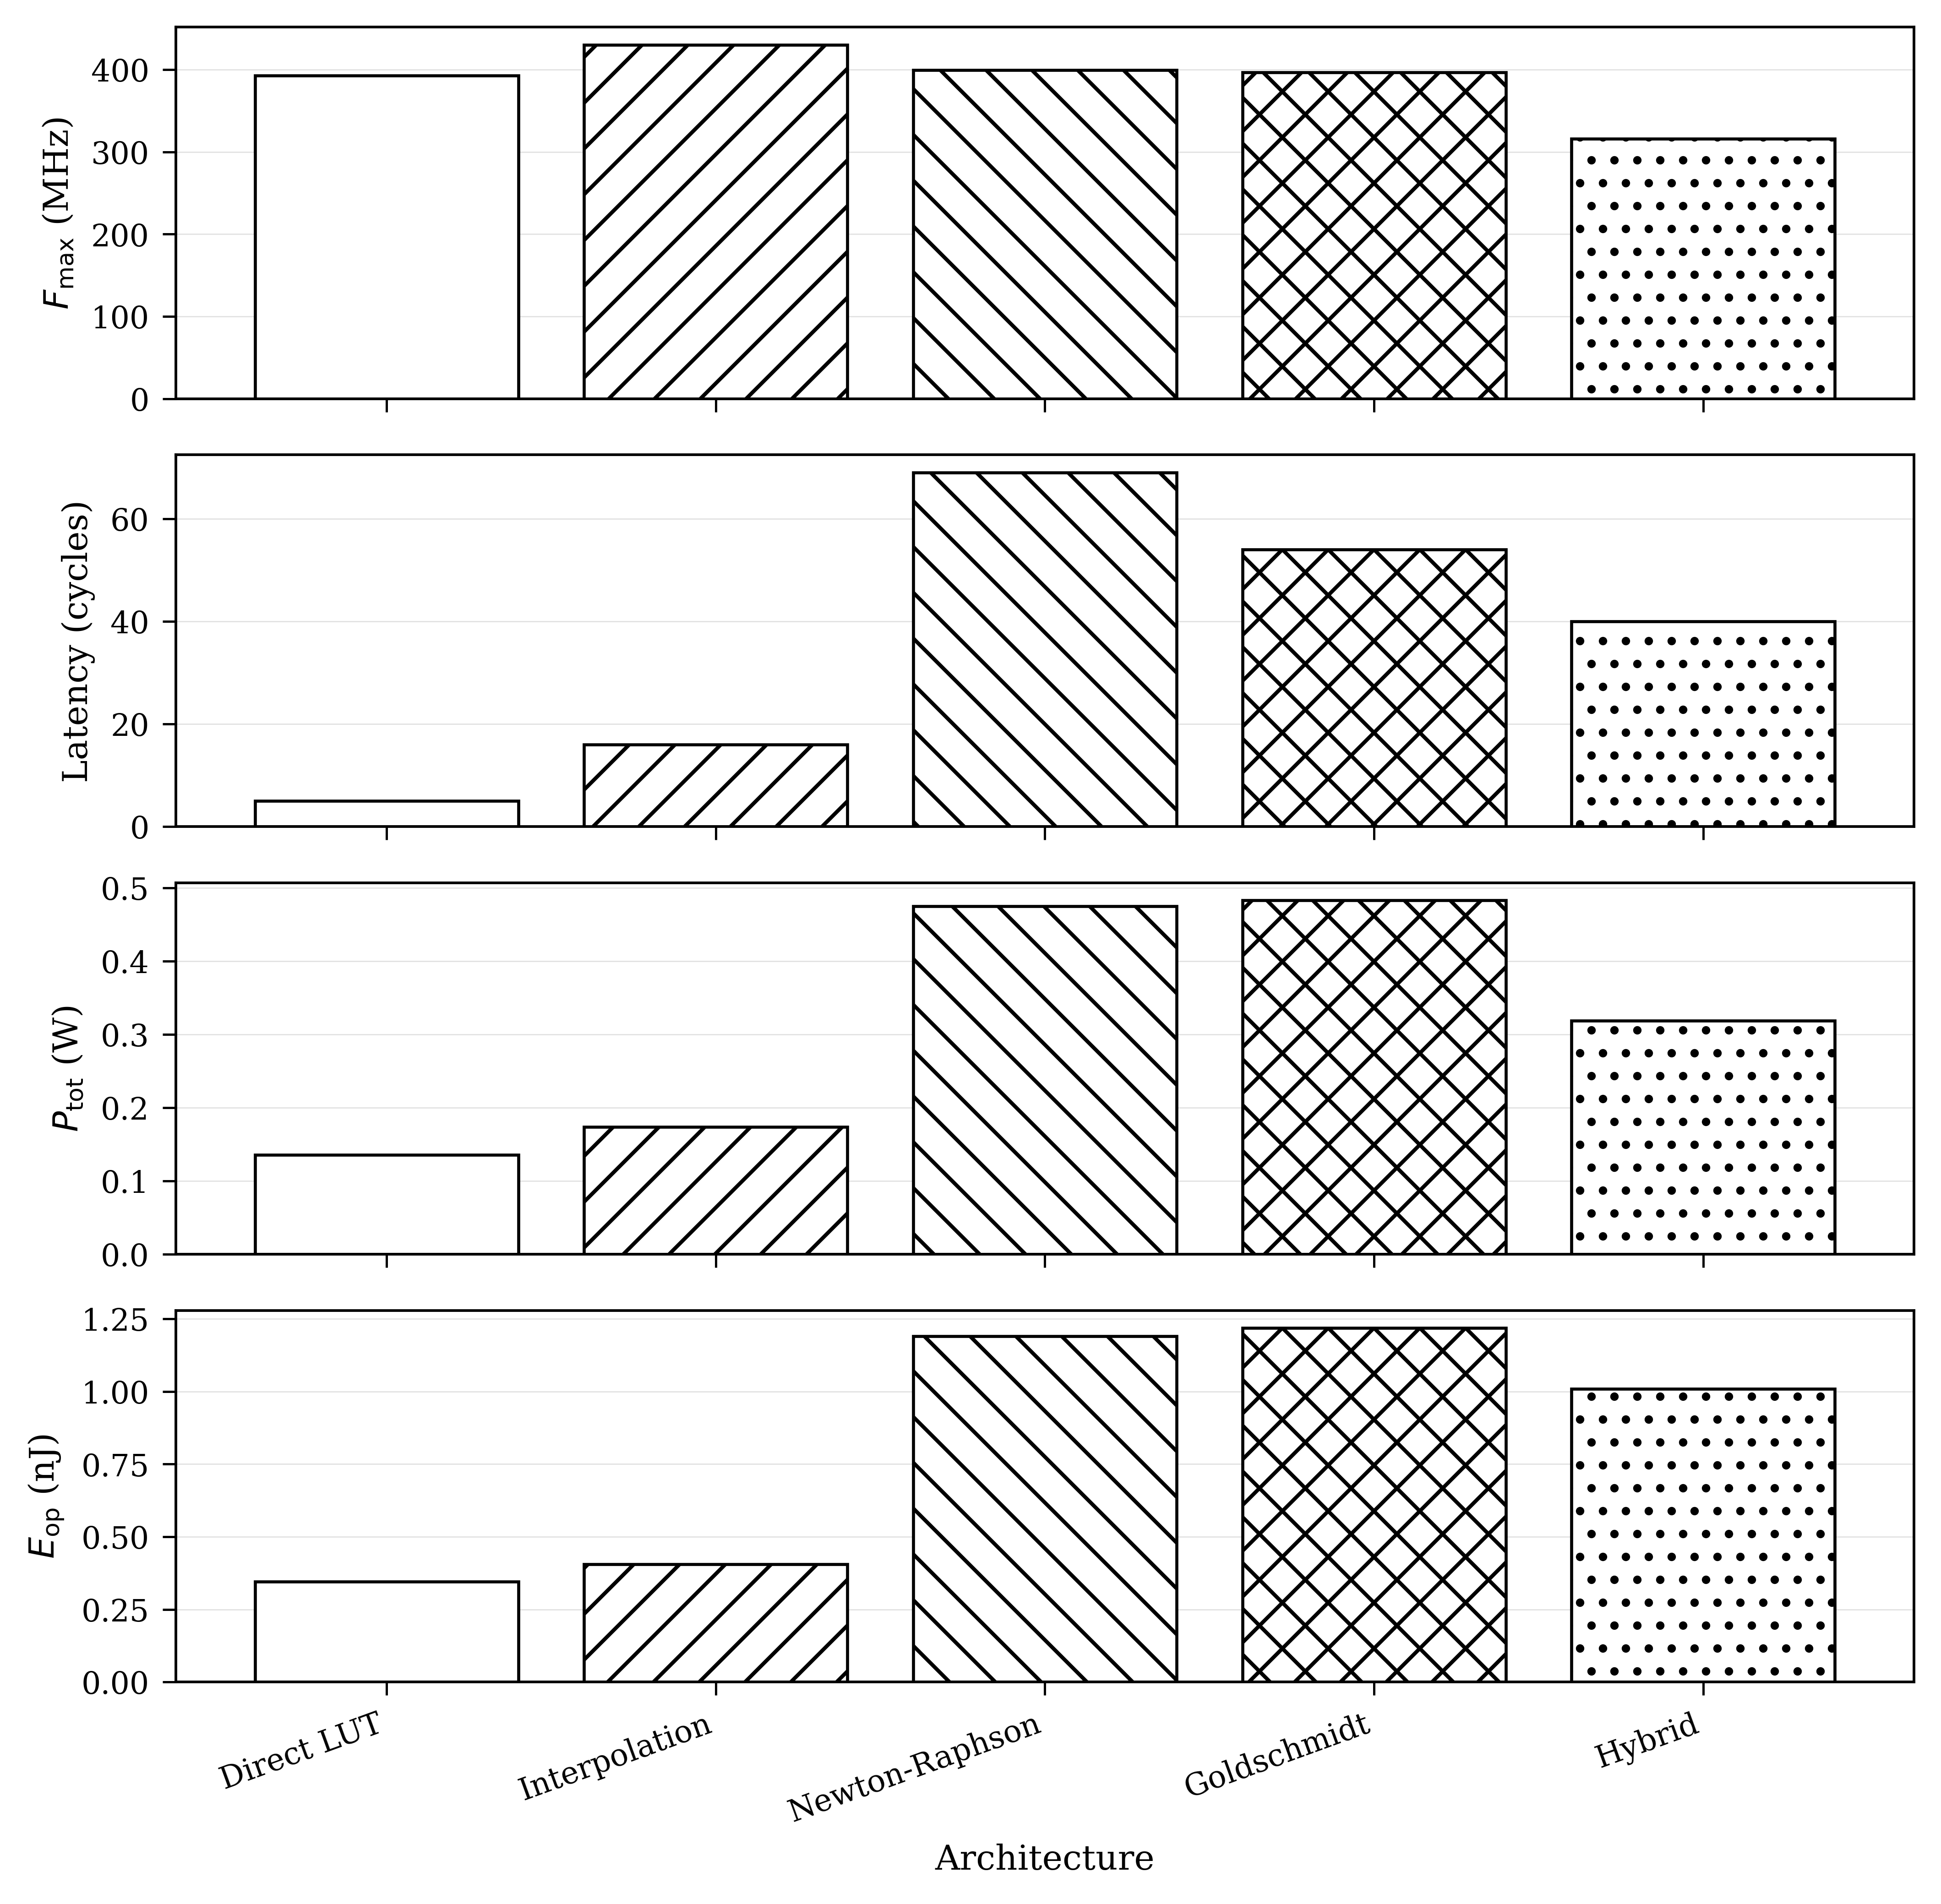
\includegraphics[width=0.49\columnwidth]{figures/q8_fmax.png}
\hfill
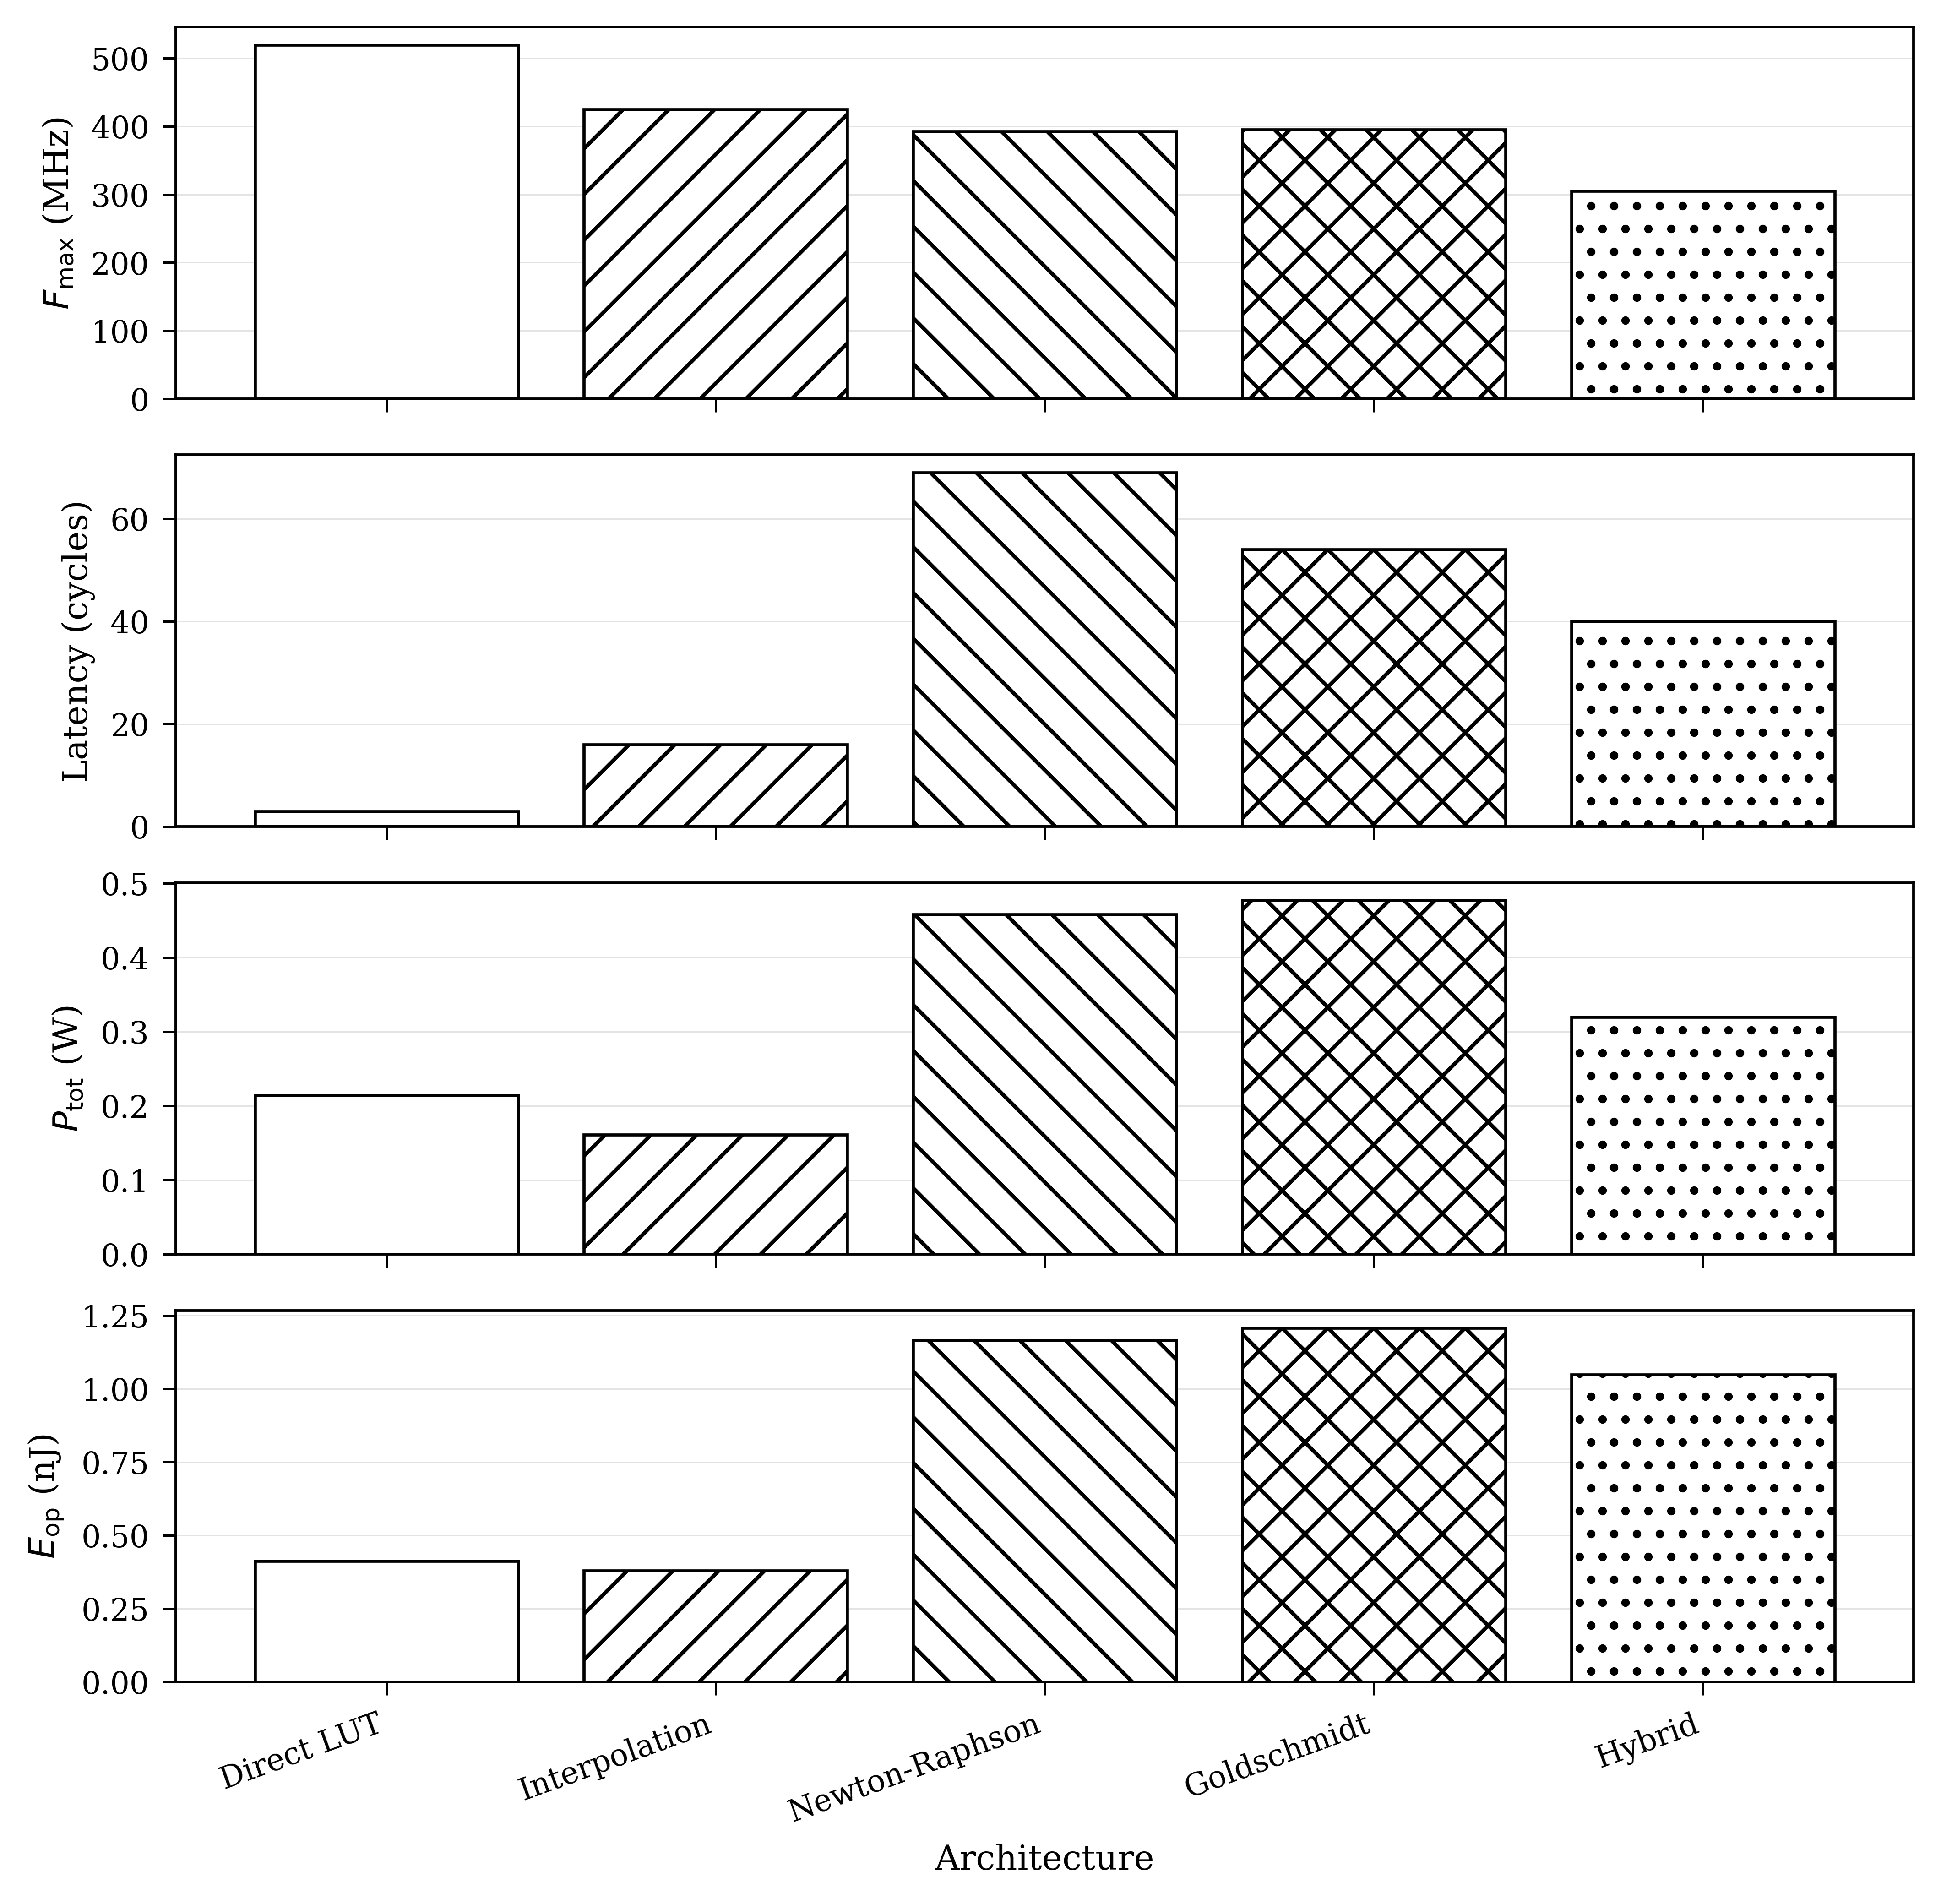
\includegraphics[width=0.49\columnwidth]{figures/q16_fmax.png}

\caption{Post-implementation $F_{\max}$ (MHz), latency (cycles), total power (W), and energy per operation (nJ/op) by architecture, Q8.24 (left) and Q16.16 (right)}
\Description{Two panels, each with four groups of bars for the five architectures. F max is 392.77 to 429.74 MHz in Q8.24 for every architecture except the hybrid at 316.06 MHz. In Q16.16 Direct LUT reaches 519.21 MHz and the hybrid is lowest at 305.06 MHz. Pipeline depth is 5 (3 in Q16.16), 16, 69, 54 and 40 cycles for Direct LUT, interpolation, Newton-Raphson, Goldschmidt and hybrid. Total power rises from 0.136 W (Direct LUT, Q8.24) to 0.483 W (Goldschmidt, Q8.24). Energy per operation rises from 0.346 to 1.219 nanojoules across the same architectures.}
\label{fig:summary}
\end{figure}

\subsection{Numerical Accuracy}
\label{sec:accuracy}

Table~\ref{tab:accuracy} summarizes the four accuracy metrics defined in Section~\ref{sec:verification} for all ten architecture/format combinations. As expected from the architectural discussion in Sections~\ref{sec:arch-directlut} through~\ref{sec:arch-gs}, the two table-based architectures exhibit the largest maximum relative error (0.098\% for Direct LUT and 0.0104\% for LUT-Interpolation, both in Q8.24), while the two full iterative architectures achieve error roughly $7\times10^{2}$ times smaller than interpolation and over $6\times10^{3}$ times smaller than the Direct LUT ($1.5\times10^{-5}$\% for Newton-Raphson and $2.0\times10^{-5}$\% for Goldschmidt, Q8.24). The Hybrid architecture, benefiting from a single refinement iteration applied to an already-interpolated seed, achieves a maximum relative error of $4.09\times10^{-4}$\%, roughly 25$\times$ worse than the full iterative architectures but more than 25$\times$ better than interpolation alone, consistent with the intermediate positioning described in Section~\ref{sec:arch-hybrid}.

\begin{table*}[H]
\caption{Numerical Accuracy Summary (1,000,000-Vector Sweep, $x \in [0.5, 2.5]$; MAE: mean absolute error, RMSE: root-mean-square error)}
\label{tab:accuracy}
\begin{tabular}{@{}llrrrr@{}}
\toprule
\textbf{Architecture} & \textbf{Format} & \textbf{Max Abs Error (real)} & \textbf{MAE (real)} & \textbf{RMSE (LSB)} & \textbf{Max Rel. Error (\%)} \\
\midrule
Direct LUT & Q8.24 & $1.950\times10^{-3}$ & $1.95\times10^{-4}$ & 5440.20 & 0.097596 \\
Direct LUT & Q16.16 & $1.892\times10^{-3}$ & $1.89\times10^{-4}$ & 20.75 & 0.094787 \\
LUT-Interpolation & Q8.24 & $2.079\times10^{-4}$ & $1.41\times10^{-7}$ & 11.70 & 0.010396 \\
LUT-Interpolation & Q16.16 & $1.831\times10^{-4}$ & $7.49\times10^{-6}$ & 0.71 & 0.009156 \\
Newton-Raphson & Q8.24 & $1.192\times10^{-7}$ & $1.21\times10^{-8}$ & 0.45 & 0.000015 \\
Newton-Raphson & Q16.16 & $1.526\times10^{-5}$ & $3.11\times10^{-6}$ & 0.45 & 0.003815 \\
Goldschmidt & Q8.24 & $1.788\times10^{-7}$ & $2.15\times10^{-8}$ & 0.62 & 0.000020 \\
Goldschmidt & Q16.16 & $3.052\times10^{-5}$ & $3.81\times10^{-6}$ & 0.51 & 0.003814 \\
Hybrid & Q8.24 & $8.166\times10^{-6}$ & $1.60\times10^{-6}$ & 38.60 & 0.000409 \\
Hybrid & Q16.16 & $7.629\times10^{-5}$ & $3.86\times10^{-6}$ & 0.59 & 0.004118 \\
\bottomrule
\end{tabular}
\end{table*}

Figs.~\ref{fig:errdist824}-\ref{fig:errdistlog824} show the distribution of signed error across all five Q8.24 architectures, first in raw LSB units and then on a log-compressed $|e|$ scale to make the tails of the heavier-tailed distributions (Direct LUT, Hybrid) visible alongside the tightly concentrated iterative architectures. The corresponding Q16.16 distributions are shown in Figs.~\ref{fig:errdist1616}-\ref{fig:errdistlog1616}.

\begin{figure}[H]
\centering
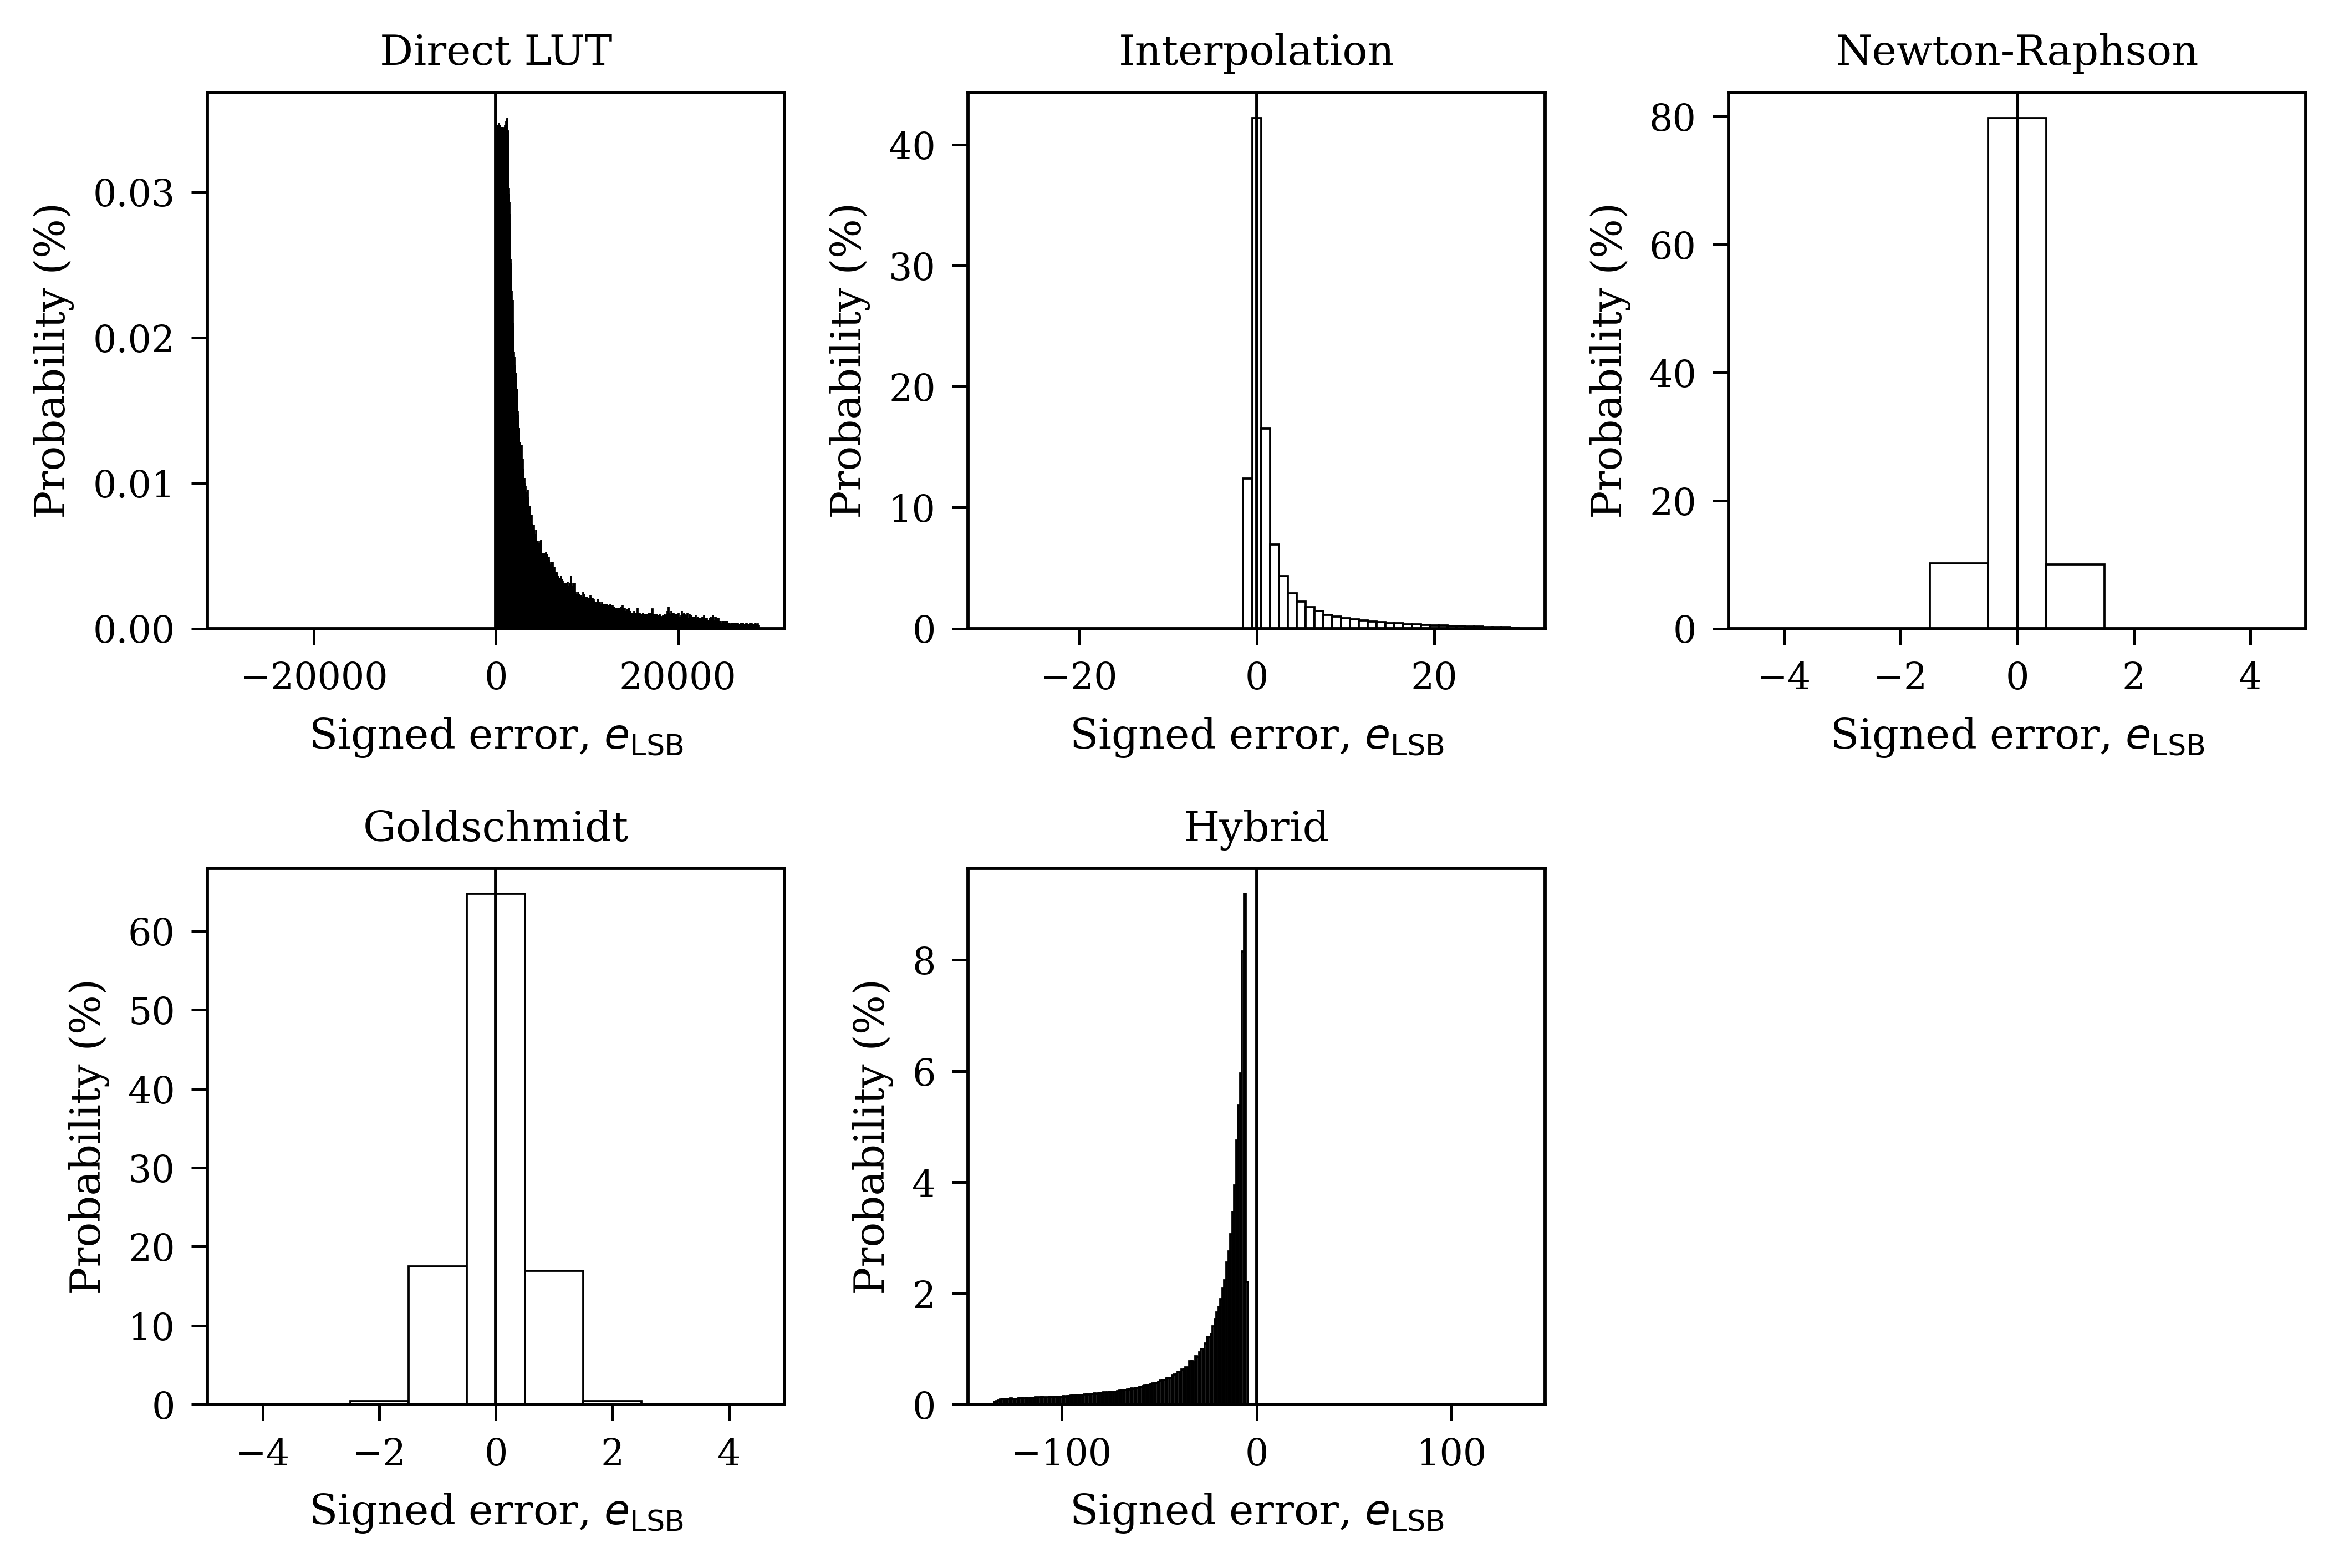
\includegraphics[width=0.85\linewidth]{figures/q8_signederror.png}
\caption{Signed error distributions (error in LSB) by architecture, Q8.24.}
\Description{Overlaid histograms on a shared LSB axis. The Direct LUT histogram is by far the widest, consistent with its RMSE of 5440 LSB. The hybrid (38.6 LSB) and interpolation (11.7 LSB) histograms are much narrower. The Newton-Raphson (0.45 LSB) and Goldschmidt (0.62 LSB) histograms are concentrated within a few LSB of zero.}
\label{fig:errdist824}
\end{figure}

\begin{figure}[H]
\centering
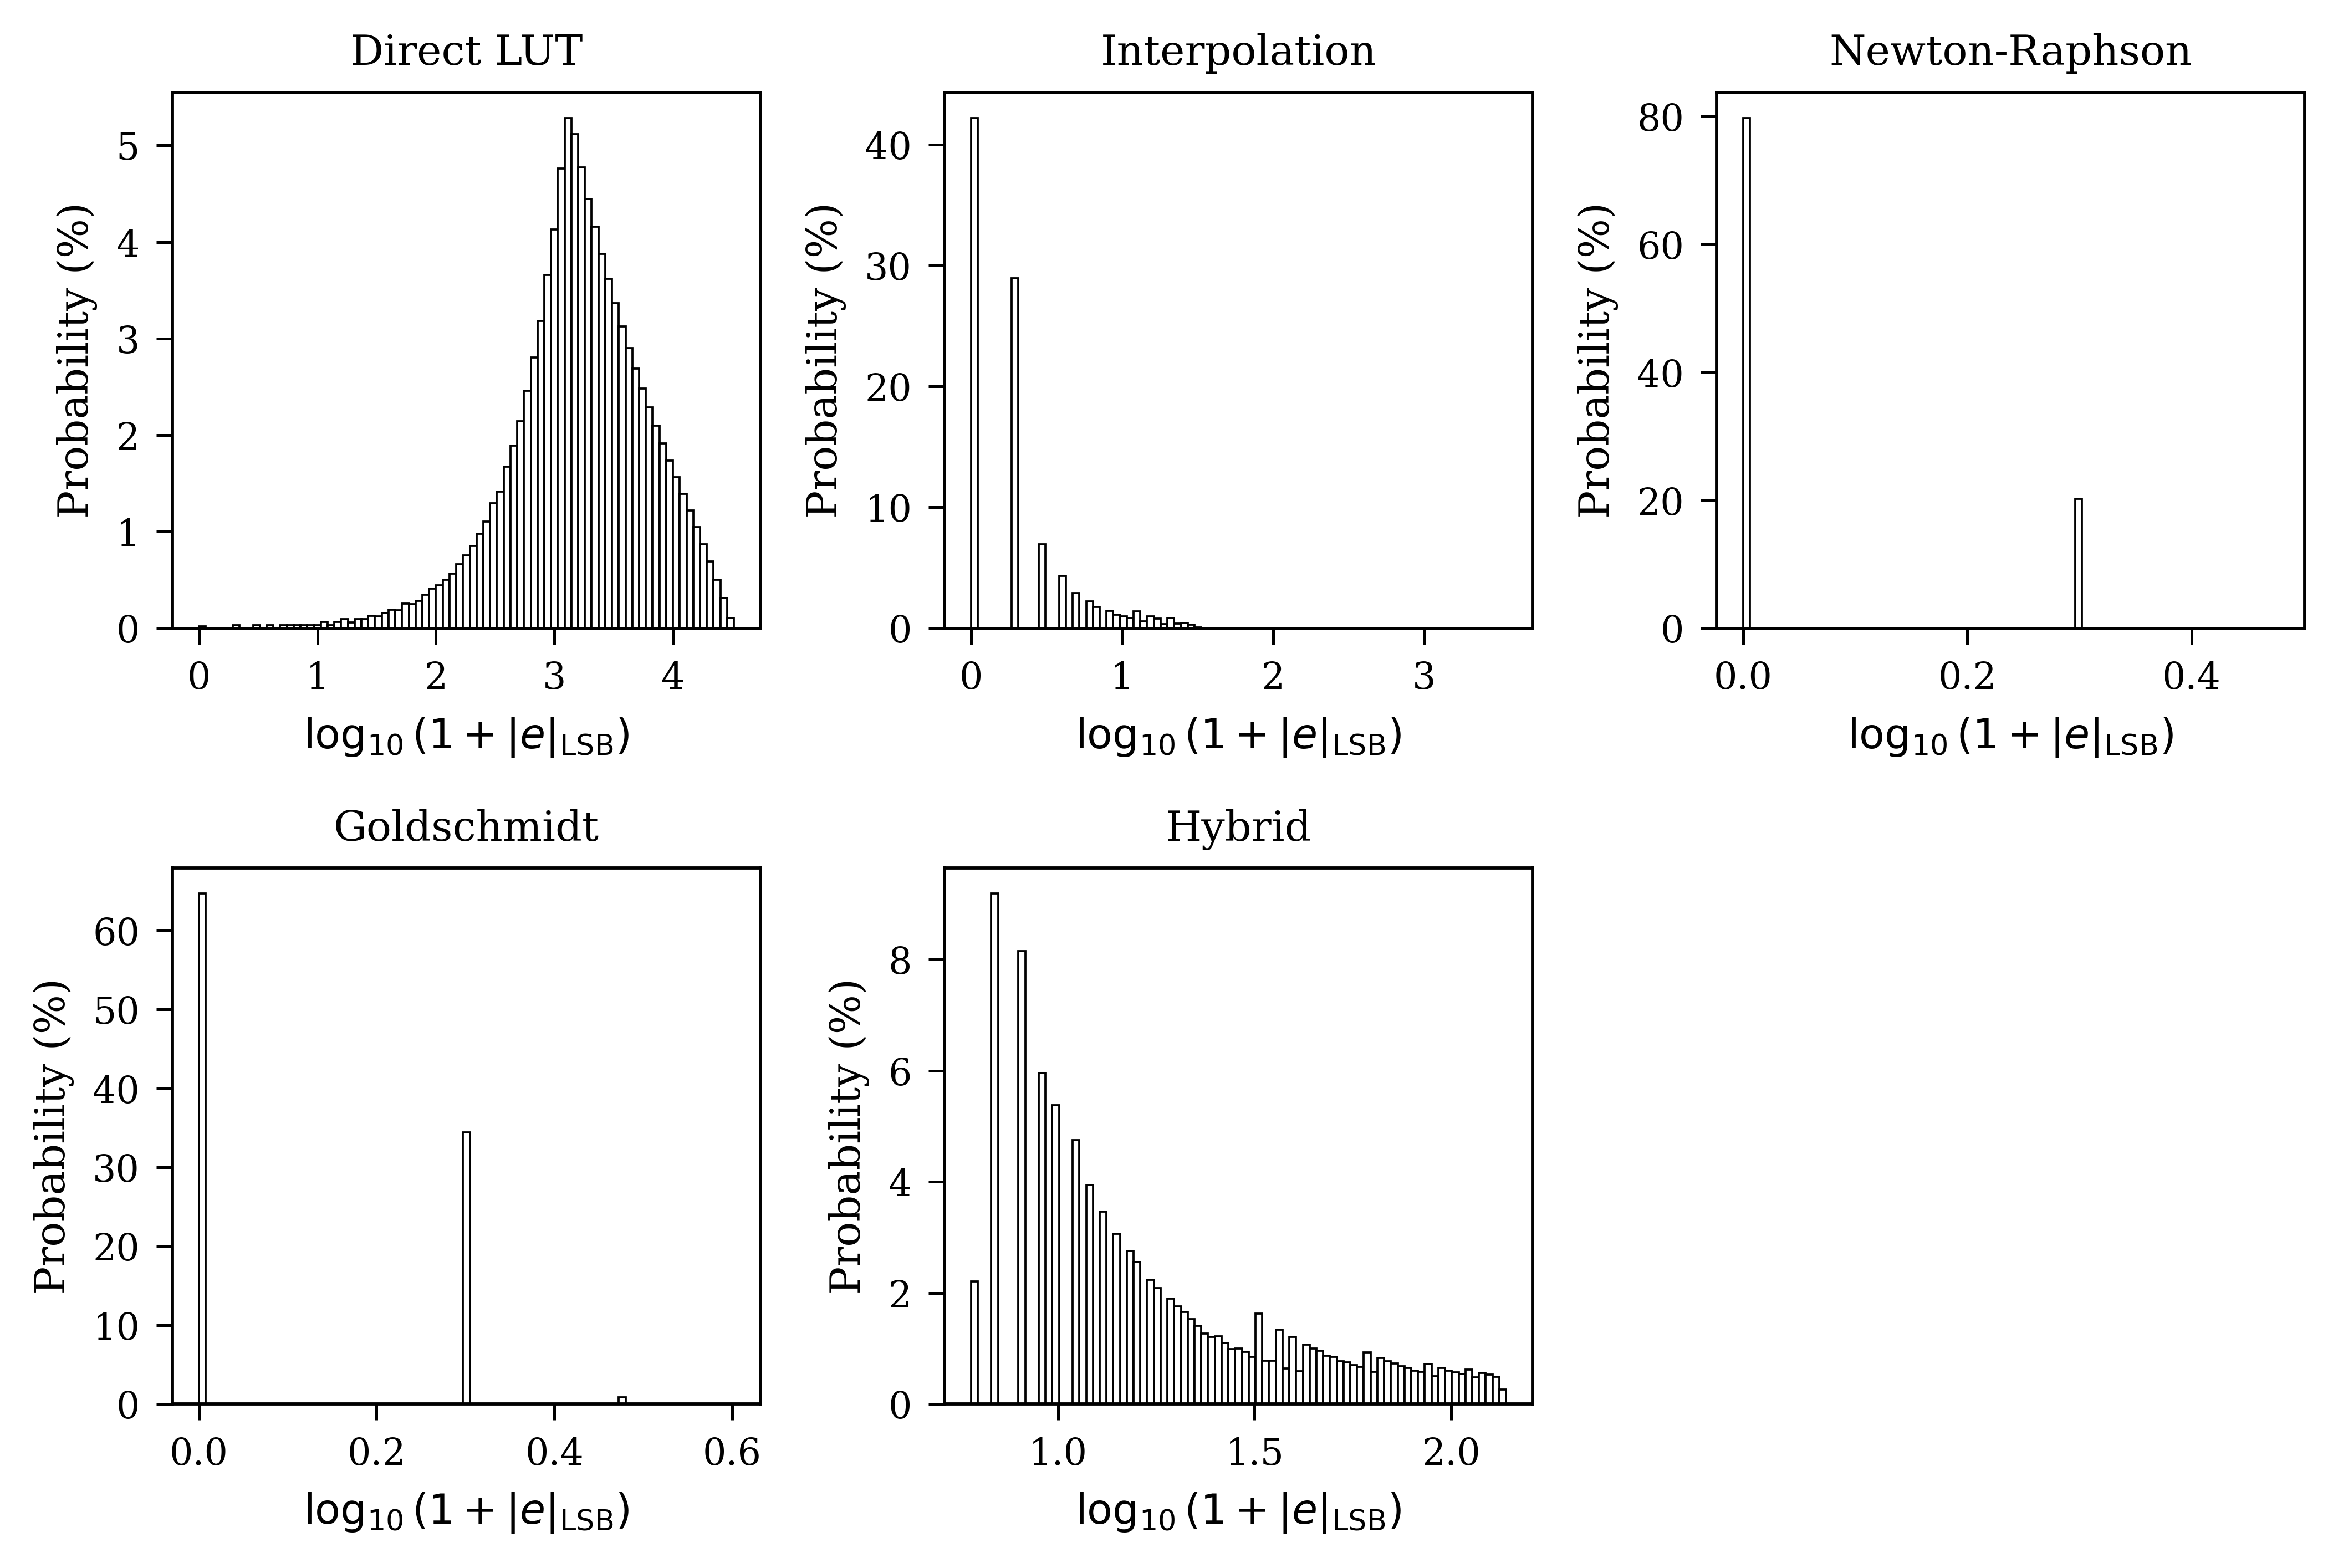
\includegraphics[width=0.85\linewidth]{figures/q8_abserr.png}
\caption{Absolute error $|e|$ distributions by architecture, Q8.24 ($\log_{10}(1+|e|)$ scale).}
\Description{Overlaid histograms on a compressed horizontal axis that makes long tails visible. The largest observed absolute errors are 0.00195 for Direct LUT, 0.000208 for interpolation, 0.0000082 for the hybrid, 0.00000018 for Goldschmidt and 0.00000012 for Newton-Raphson. On this axis the Direct LUT and hybrid histograms extend far to the right of the two iterative architectures.}
\label{fig:errdistlog824}
\end{figure}

Fig.~\ref{fig:zerolsb824} decomposes the error population for each architecture into the fraction of outputs with zero LSB error relative to the quantized fixed-point reference and the distribution of nonzero errors. The zero-LSB fraction varies substantially across the architectures. Newton-Raphson and Goldschmidt produce exact agreement with the quantized fixed-point reference for a large fraction of test vectors, whereas the Hybrid architecture exhibits predominantly nonzero errors despite its substantially lower maximum relative error than the interpolation-only design.

\begin{figure}[H]
\centering
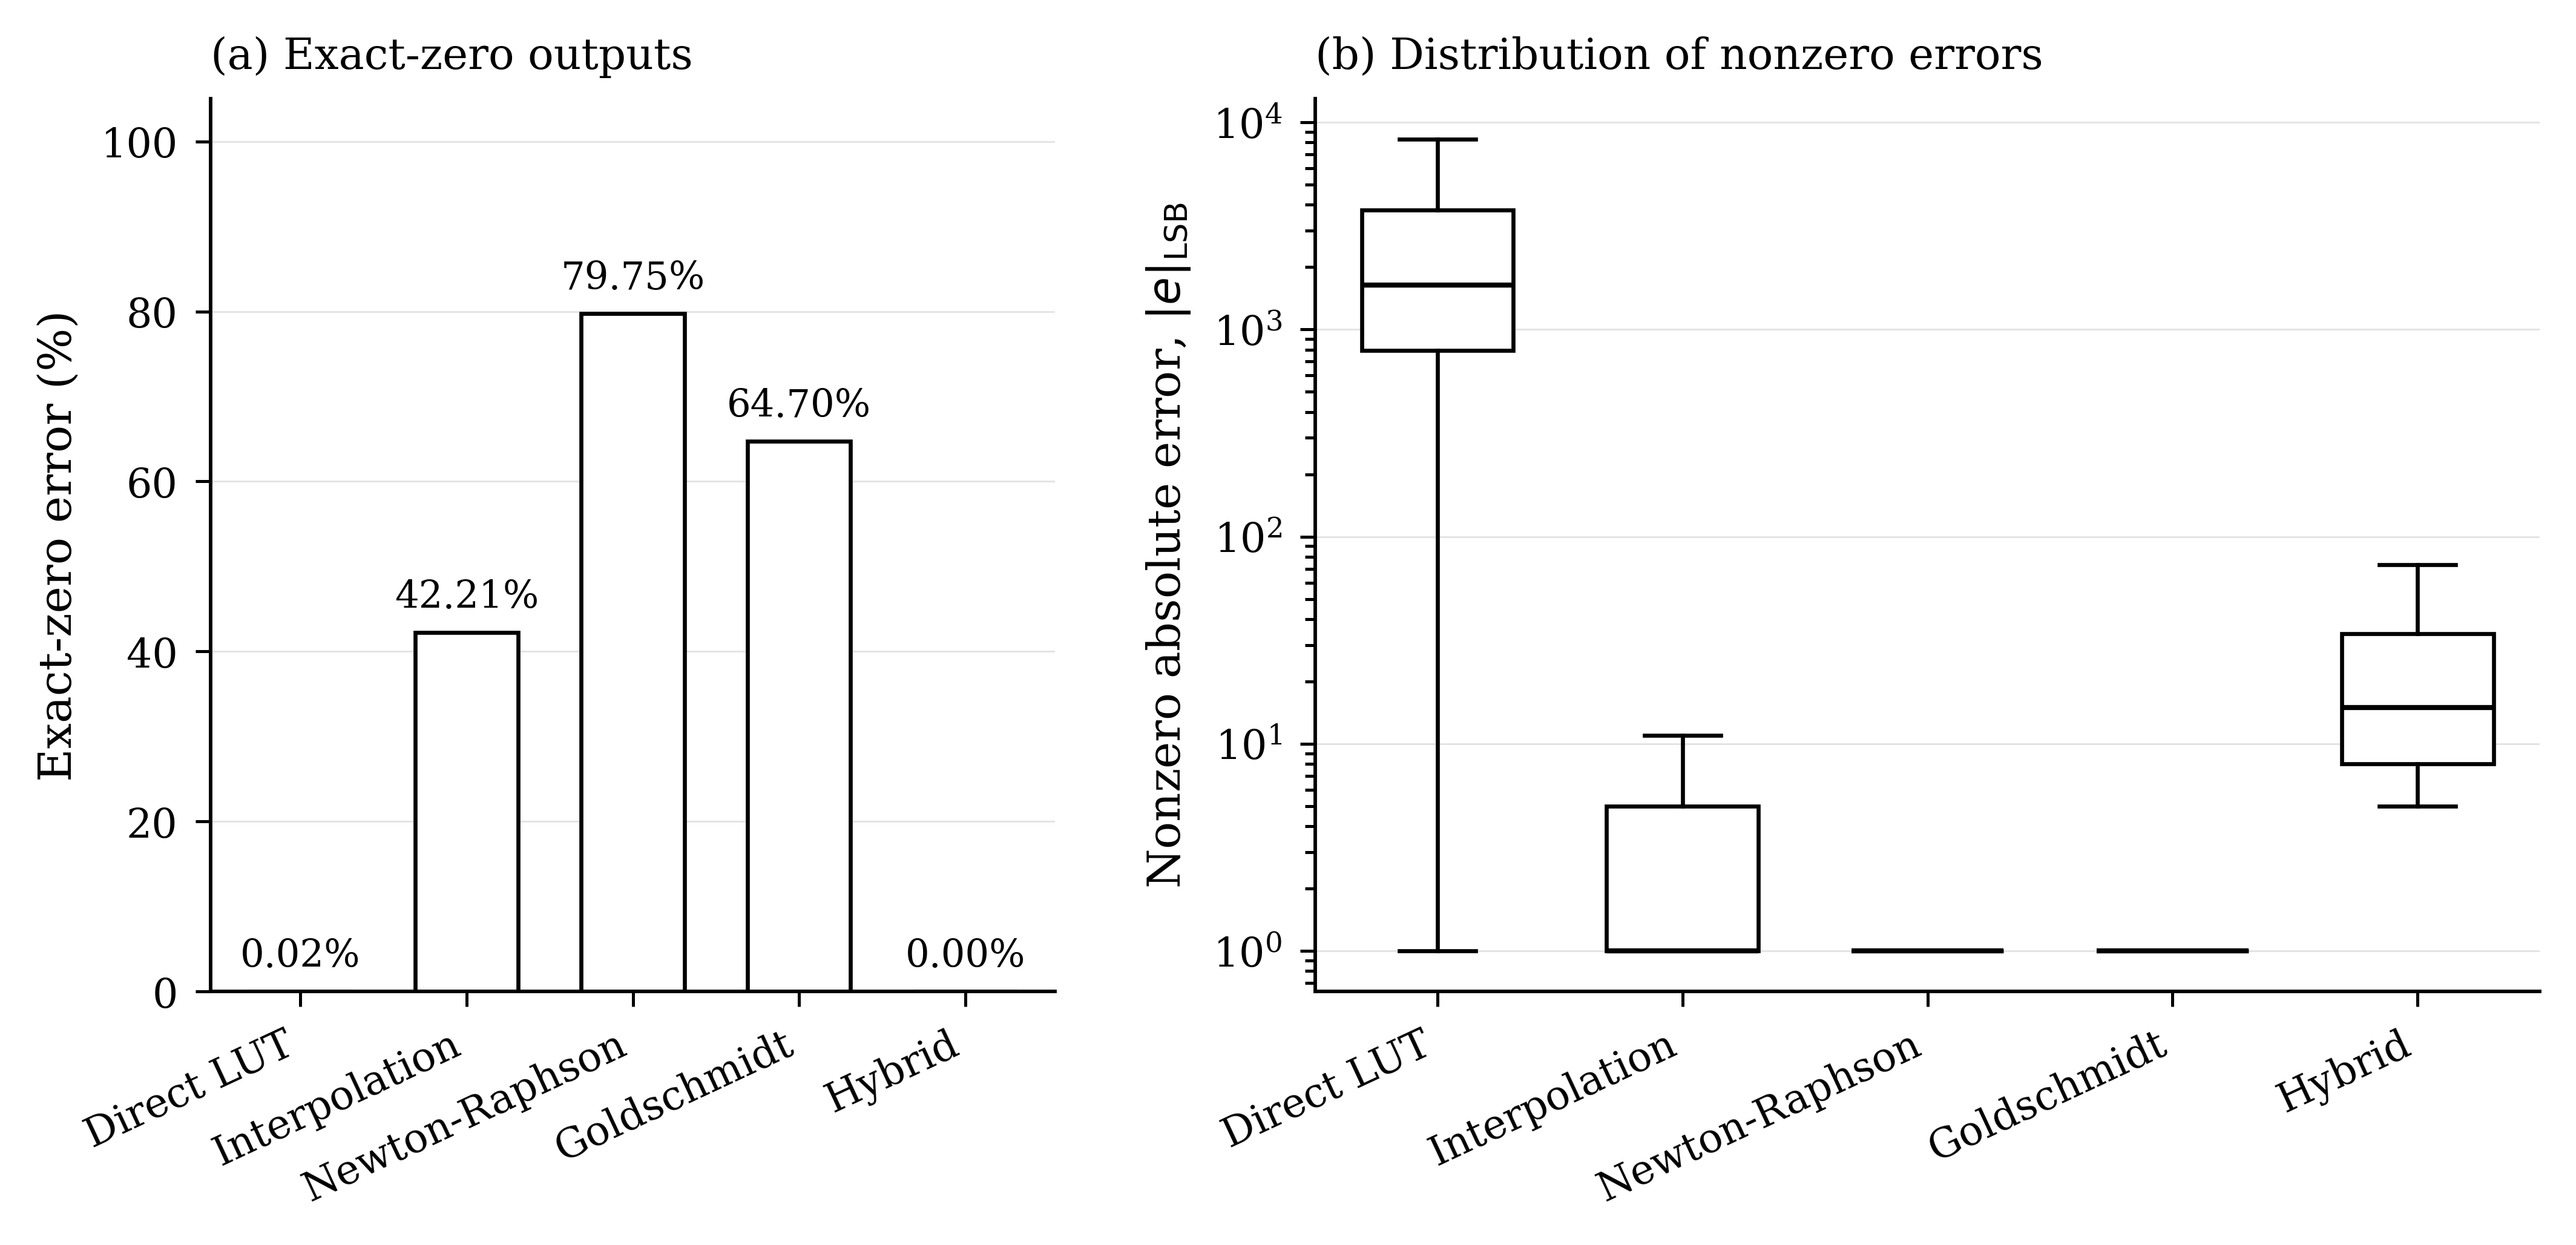
\includegraphics[width=\linewidth]{figures/q8_zeroerr.png}
\caption{Zero-LSB output fraction and distribution of nonzero signed errors (LSB) by architecture, Q8.24.}
\Description{Two views per architecture. The zero-LSB fraction is large for Newton-Raphson and Goldschmidt, so most of their outputs match the quantized reference exactly. It is small for the hybrid, whose outputs are predominantly nonzero. The nonzero errors of the two iterative architectures stay within a few LSB, while those of Direct LUT extend to tens of thousands of LSB (a maximum absolute error of 0.00195 corresponds to about 32,700 LSB).}
\label{fig:zerolsb824}
\end{figure}

Fig.~\ref{fig:maxrelerr824} shows how the maximum relative error varies as a function of the input value $x$ across the domain $[0.5, 2.5]$. For all five architectures, error is concentrated toward the lower end of the input domain, where the local slope of $1/x$ is steepest and a fixed quantization step in $x$ therefore maps to a larger quantization step in $1/x$; error decreases monotonically (Direct LUT) or in a sawtooth pattern tied to breakpoint/table boundaries (Interpolation, Goldschmidt, Hybrid) as $x$ increases toward 2.5.

\begin{figure}[H]
\centering
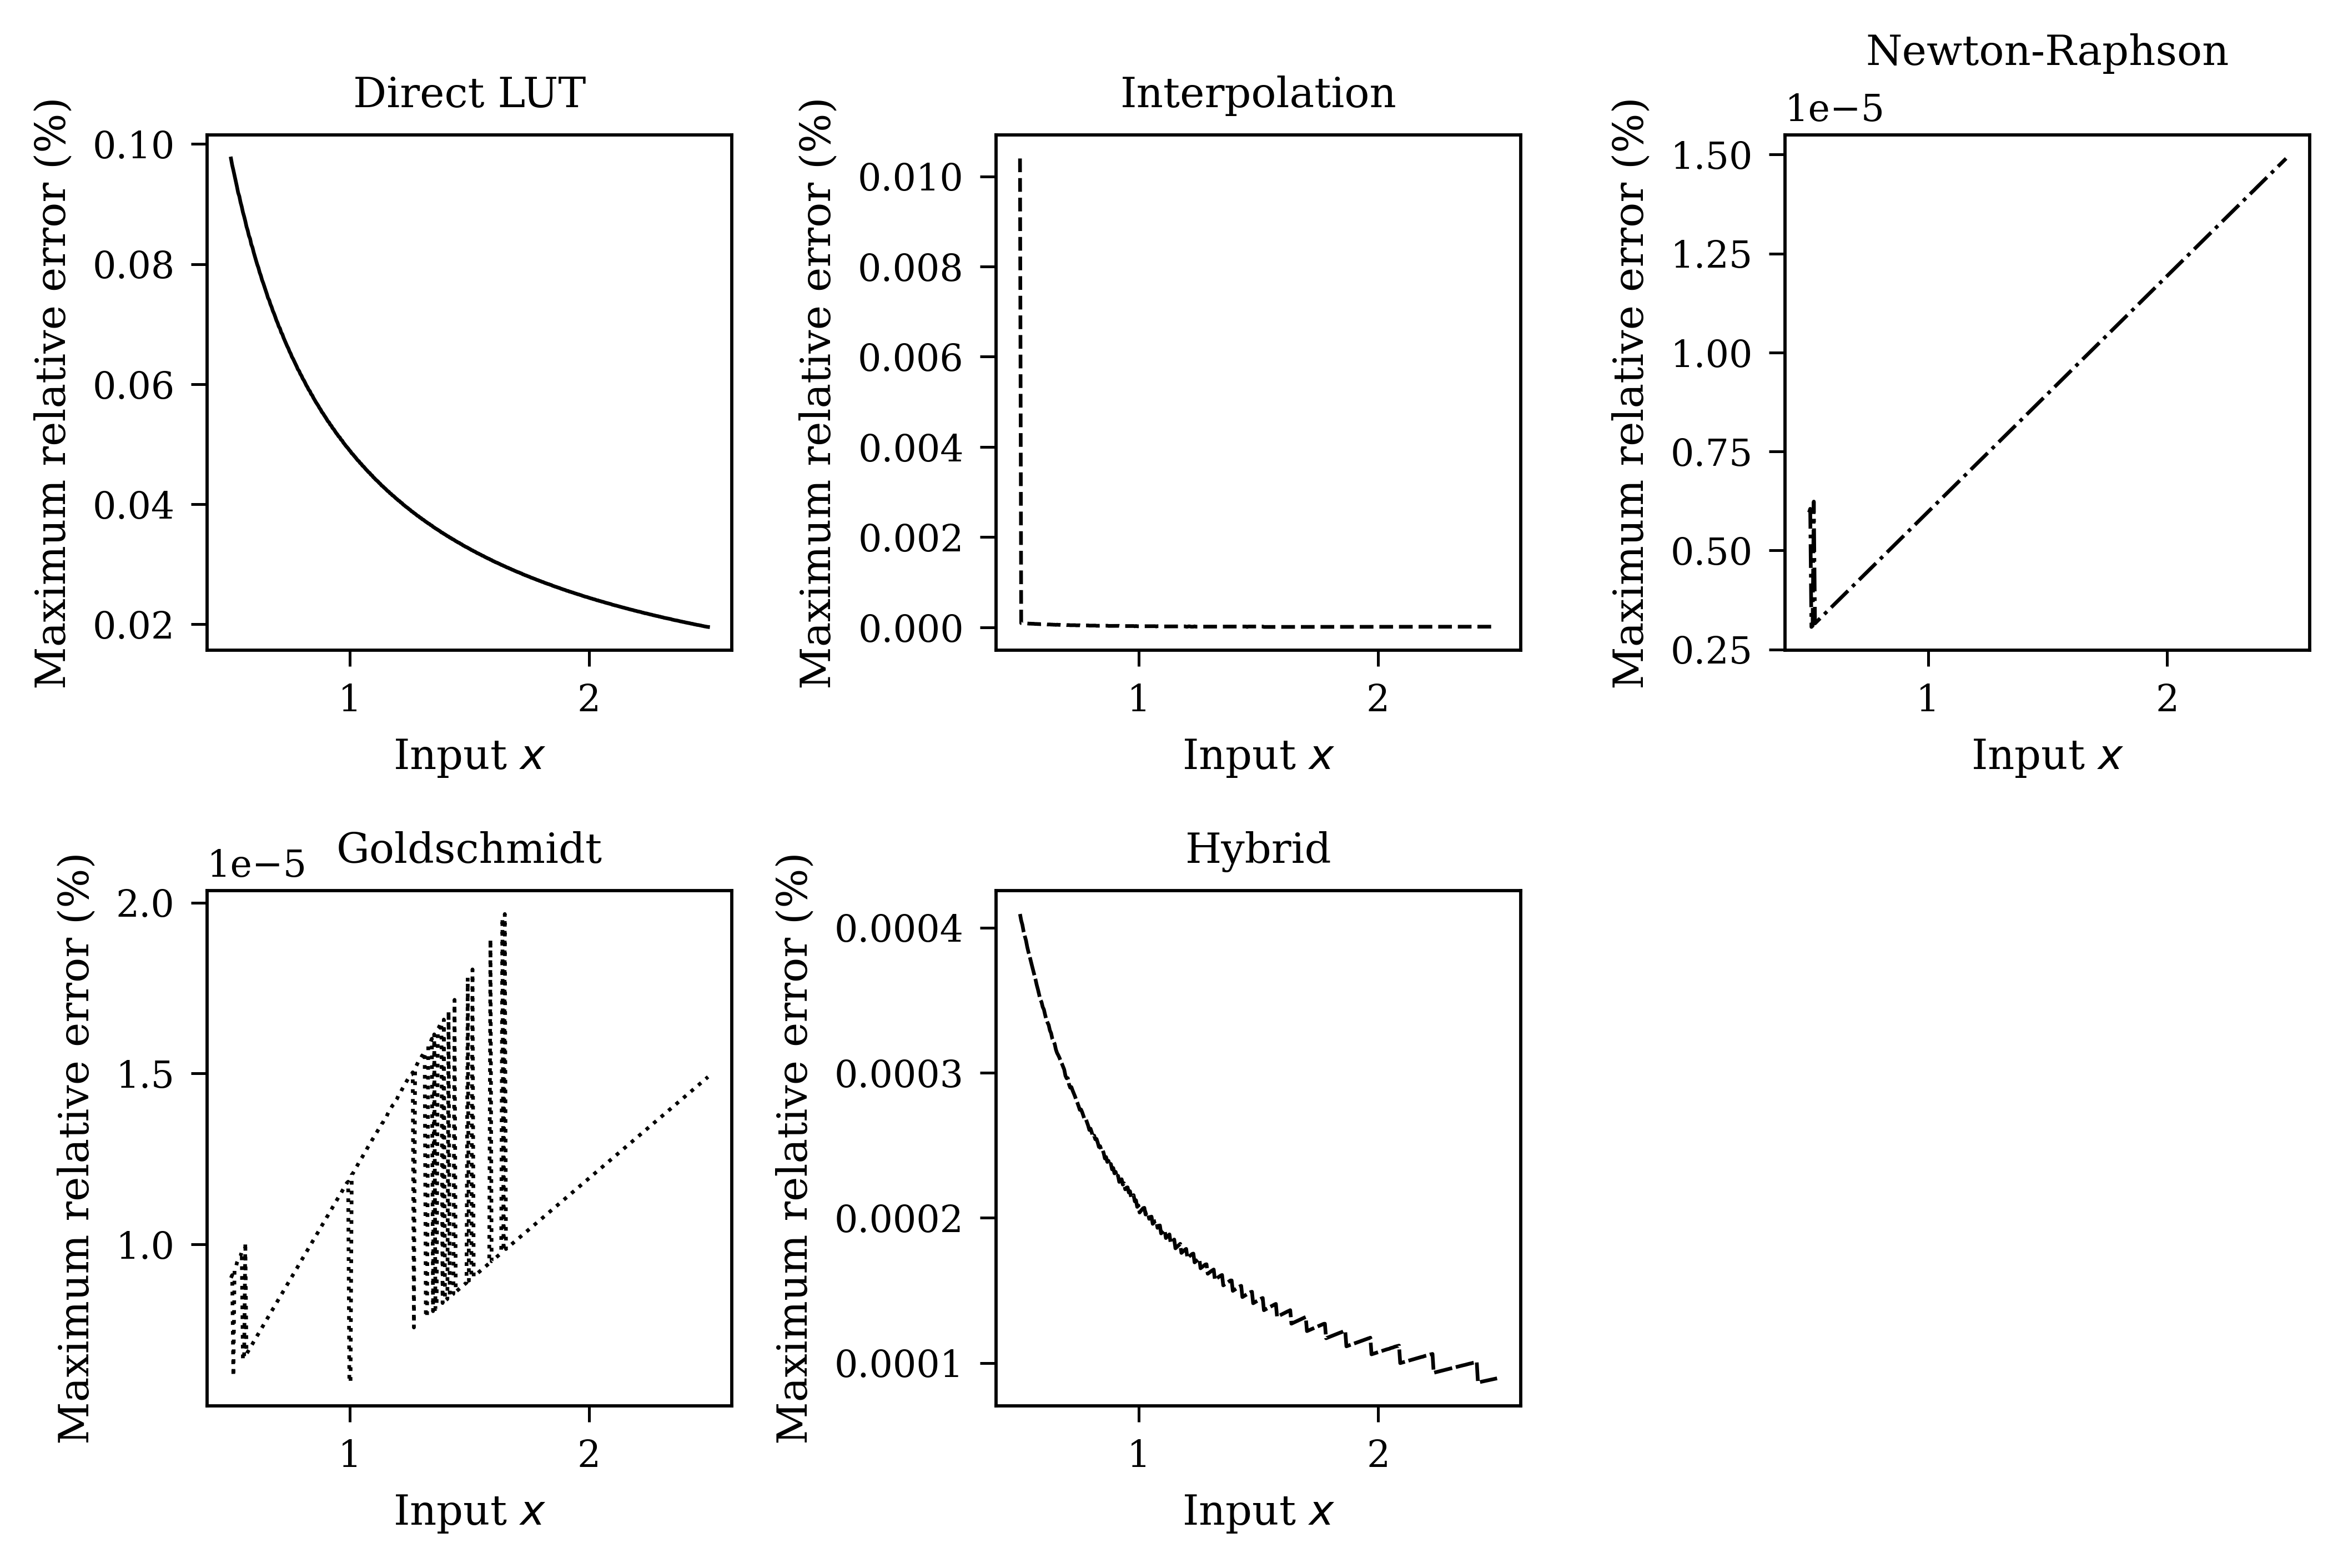
\includegraphics[width=\linewidth]{figures/q8_relerr.png}
\caption{Maximum relative error (\%) as a function of input value $x$, by architecture, Q8.24.}
\Description{Line plot of relative error against x from 0.5 to 2.5. The Direct LUT curve is highest, peaking near 0.098 percent at x equal to 0.5 and falling steadily toward x equal to 2.5. The interpolation curve peaks near 0.0104 percent and the hybrid near 0.0004 percent, both with a sawtooth shape tied to table boundaries. The Newton-Raphson and Goldschmidt curves lie at the bottom of the plot, at or below about 0.00002 percent.}
\label{fig:maxrelerr824}
\end{figure}

Fig.~\ref{fig:warmup824} shows the pipeline warm-up transient discussed in Section~\ref{sec:verification}: for each architecture, the first $N_{cycles}$ output samples (shaded) correspond to the pipeline fill period and do not represent valid steady-state outputs; these samples are excluded from all summary statistics reported in Table~\ref{tab:accuracy}. Fig.~\ref{fig:percentile824} presents the complementary cumulative view, showing absolute error as a function of output percentile across the full one-million-vector sweep, which makes clear that all five architectures' worst-case error is concentrated in a small percentile tail rather than being representative of typical-case behavior.

\begin{figure}[H]
\centering
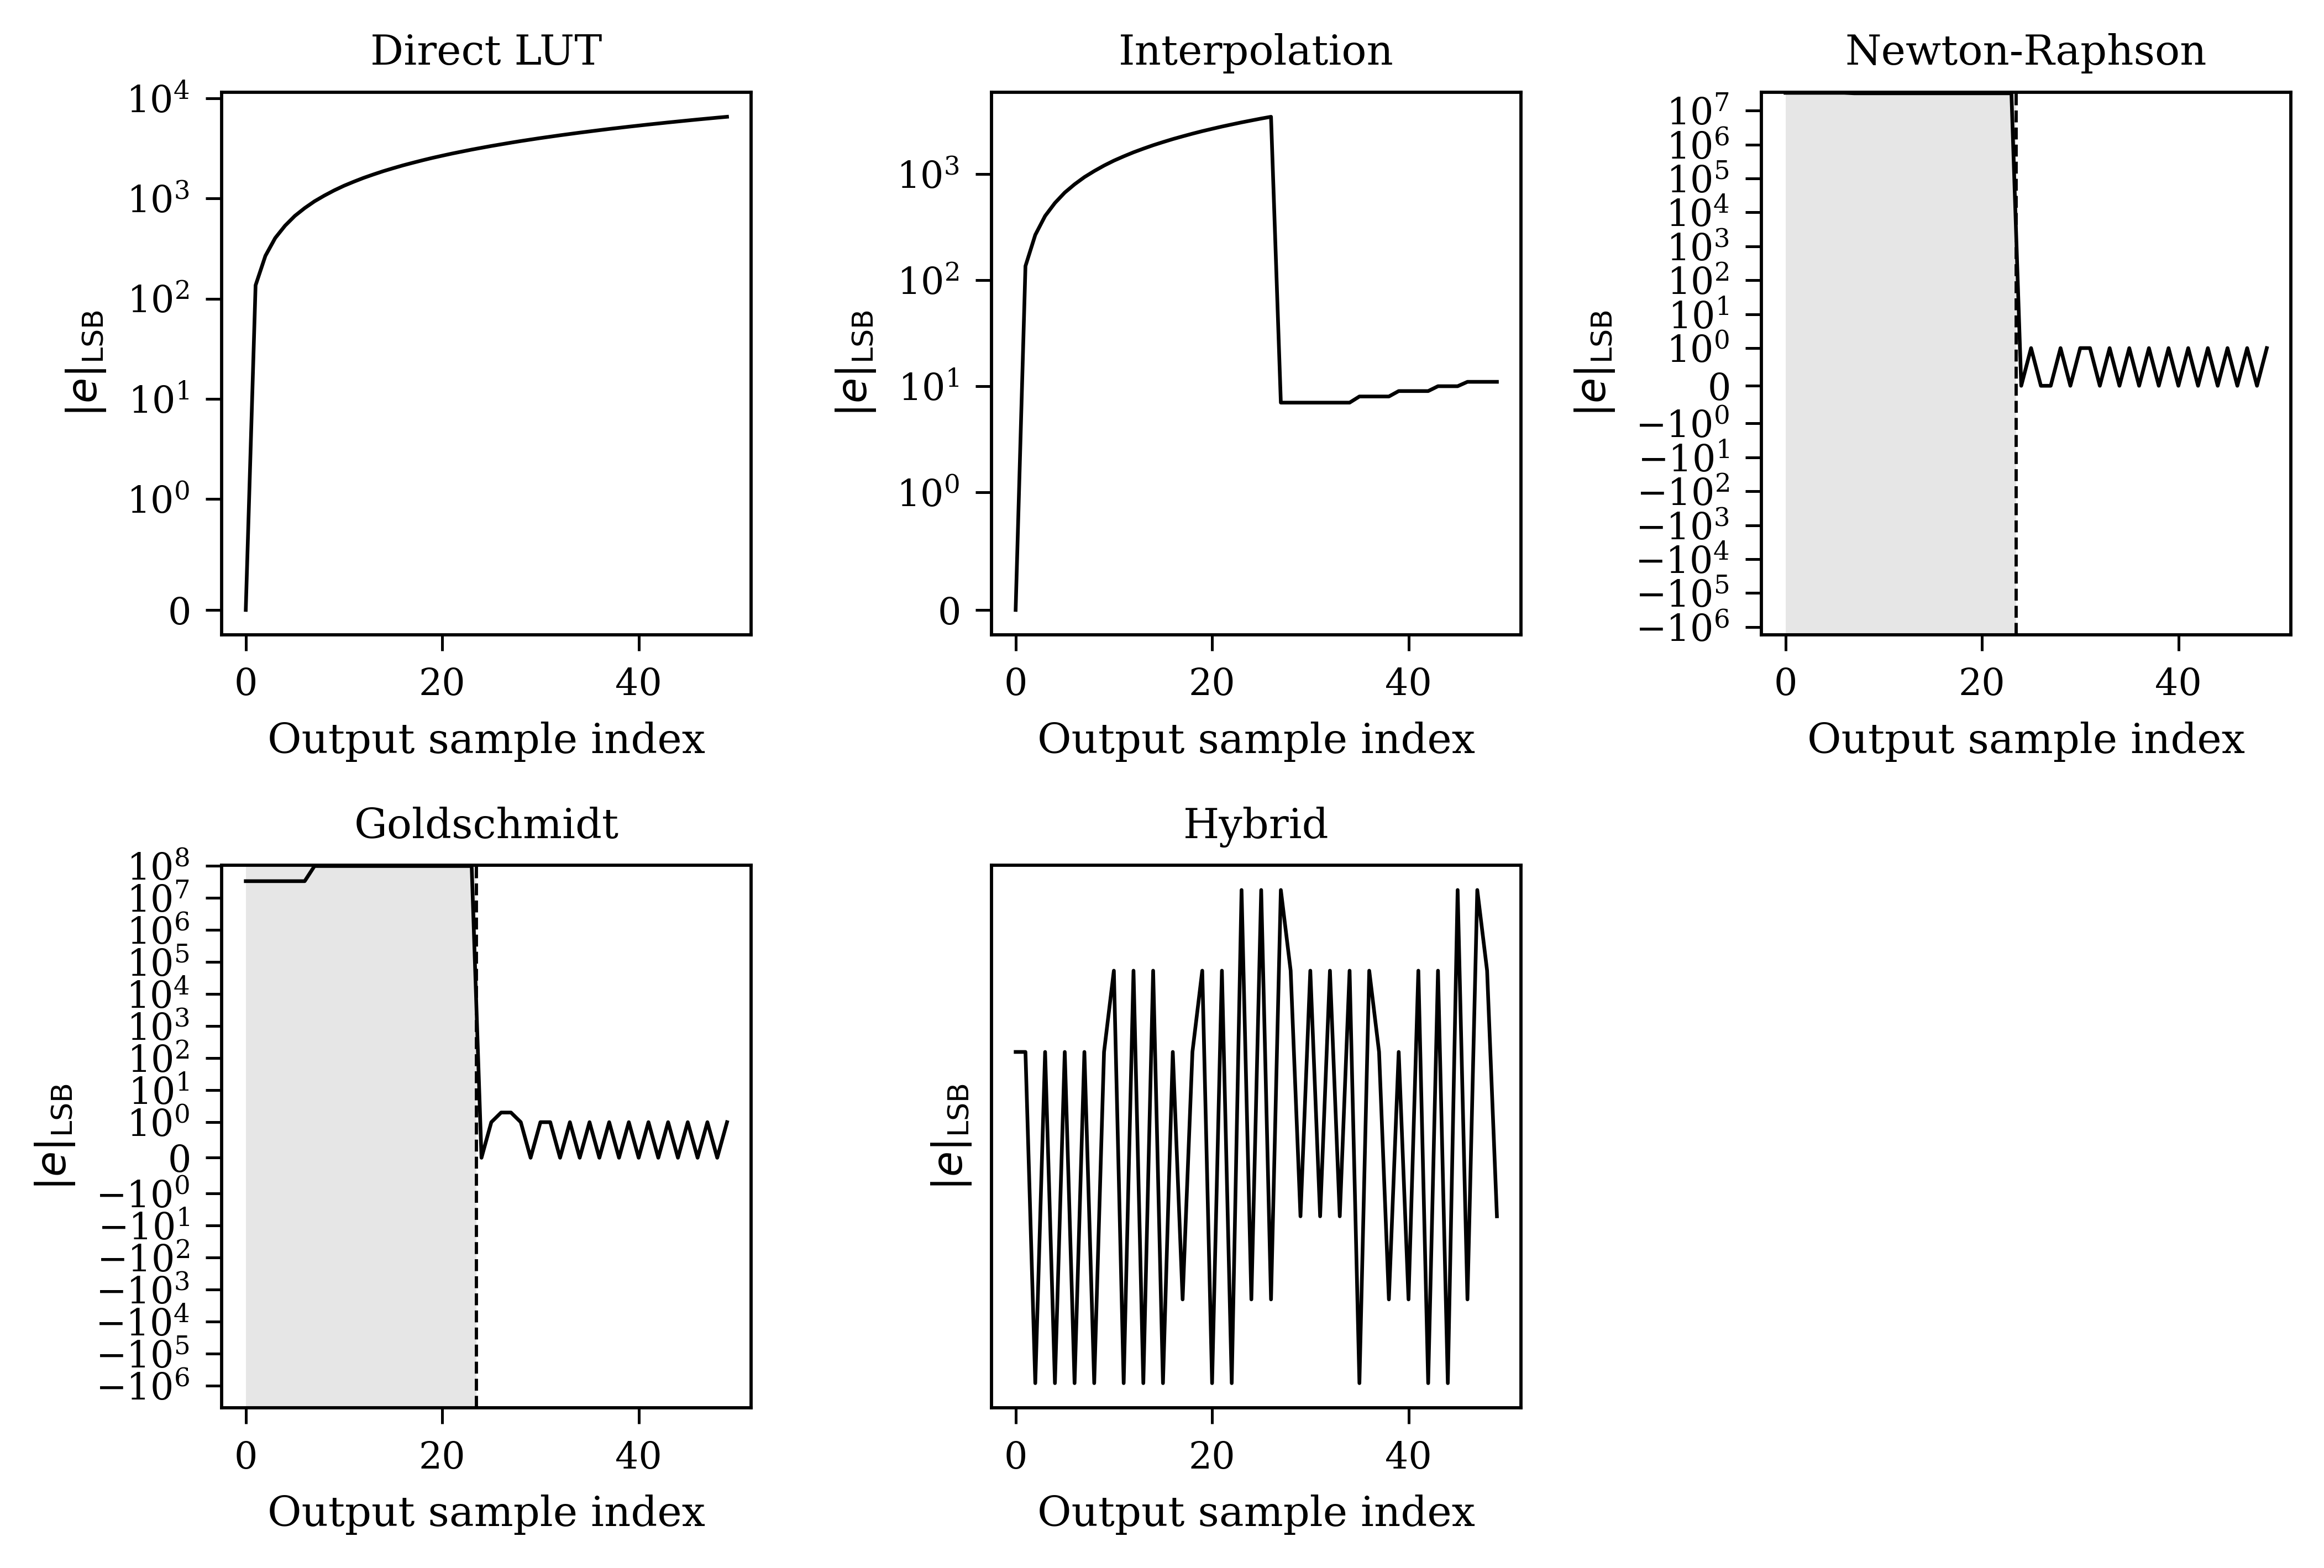
\includegraphics[width=0.9\linewidth]{figures/q8_pipelinewarmup.png}
\caption{Output error during the pipeline warm-up transient by architecture (shaded region: pipeline fill period), Q8.24.}
\Description{Time-series traces of output error over the first samples. The shaded fill period differs by architecture: 5 samples for Direct LUT, 16 for interpolation, 40 for the hybrid, 54 for Goldschmidt and 69 for Newton-Raphson. Outputs inside the shaded region are not valid results, and every trace settles to its steady-state error level once the shading ends.}
\label{fig:warmup824}
\end{figure}

\begin{figure}[H]
\centering
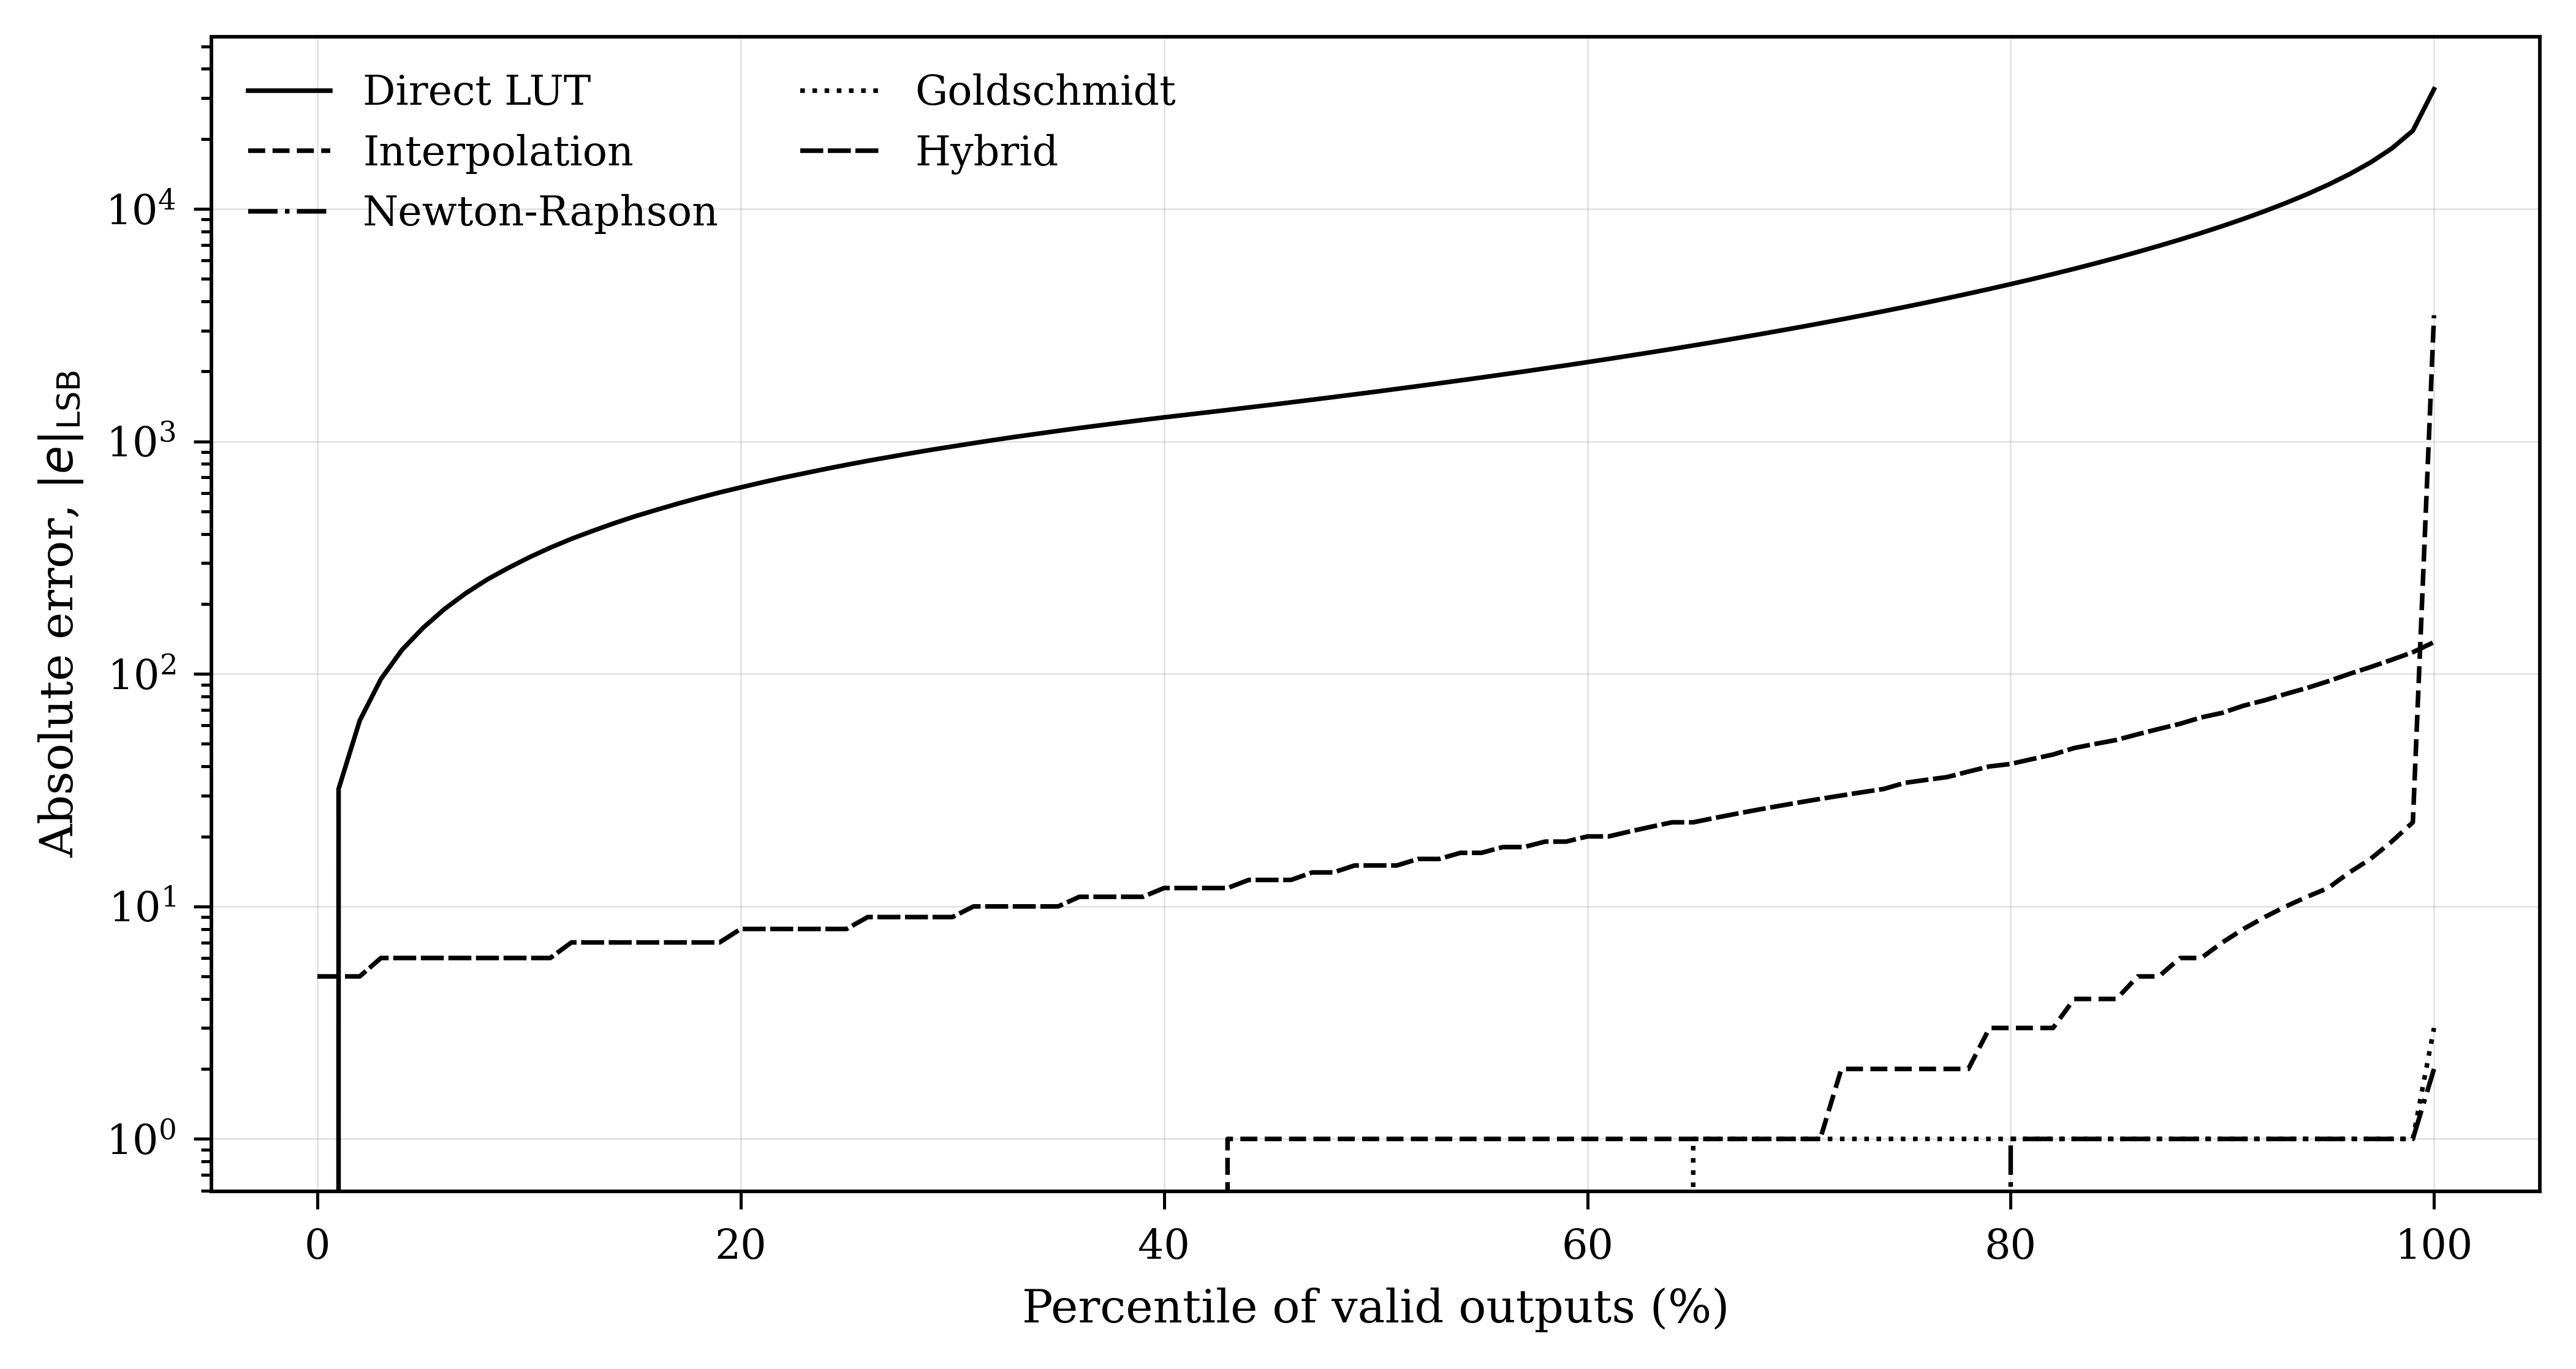
\includegraphics[width=0.9\linewidth]{figures/q8_errorpercentile.png}
\caption{Absolute error (real-valued) as a function of output percentile, all architectures, Q8.24.}
\Description{Curves of absolute error against output percentile, ordered by architecture accuracy. Newton-Raphson and Goldschmidt lie lowest, with maximum absolute errors of 0.00000012 and 0.00000018. The hybrid and interpolation curves follow, with maxima of 0.0000082 and 0.000208, and Direct LUT is highest at 0.00195. Each curve stays low for most percentiles and rises only in the final tail.}
\label{fig:percentile824}
\end{figure}

The corresponding Q16.16 error-distribution, worst-case, warm-up, and percentile figures are reproduced in Figs.~\ref{fig:errdist1616}-\ref{fig:percentile1616} for direct comparison against the Q8.24 results above; the cross-format differences visible between these figure pairs are discussed quantitatively in Section~\ref{sec:crossformat}.

\begin{figure}[H]
\centering
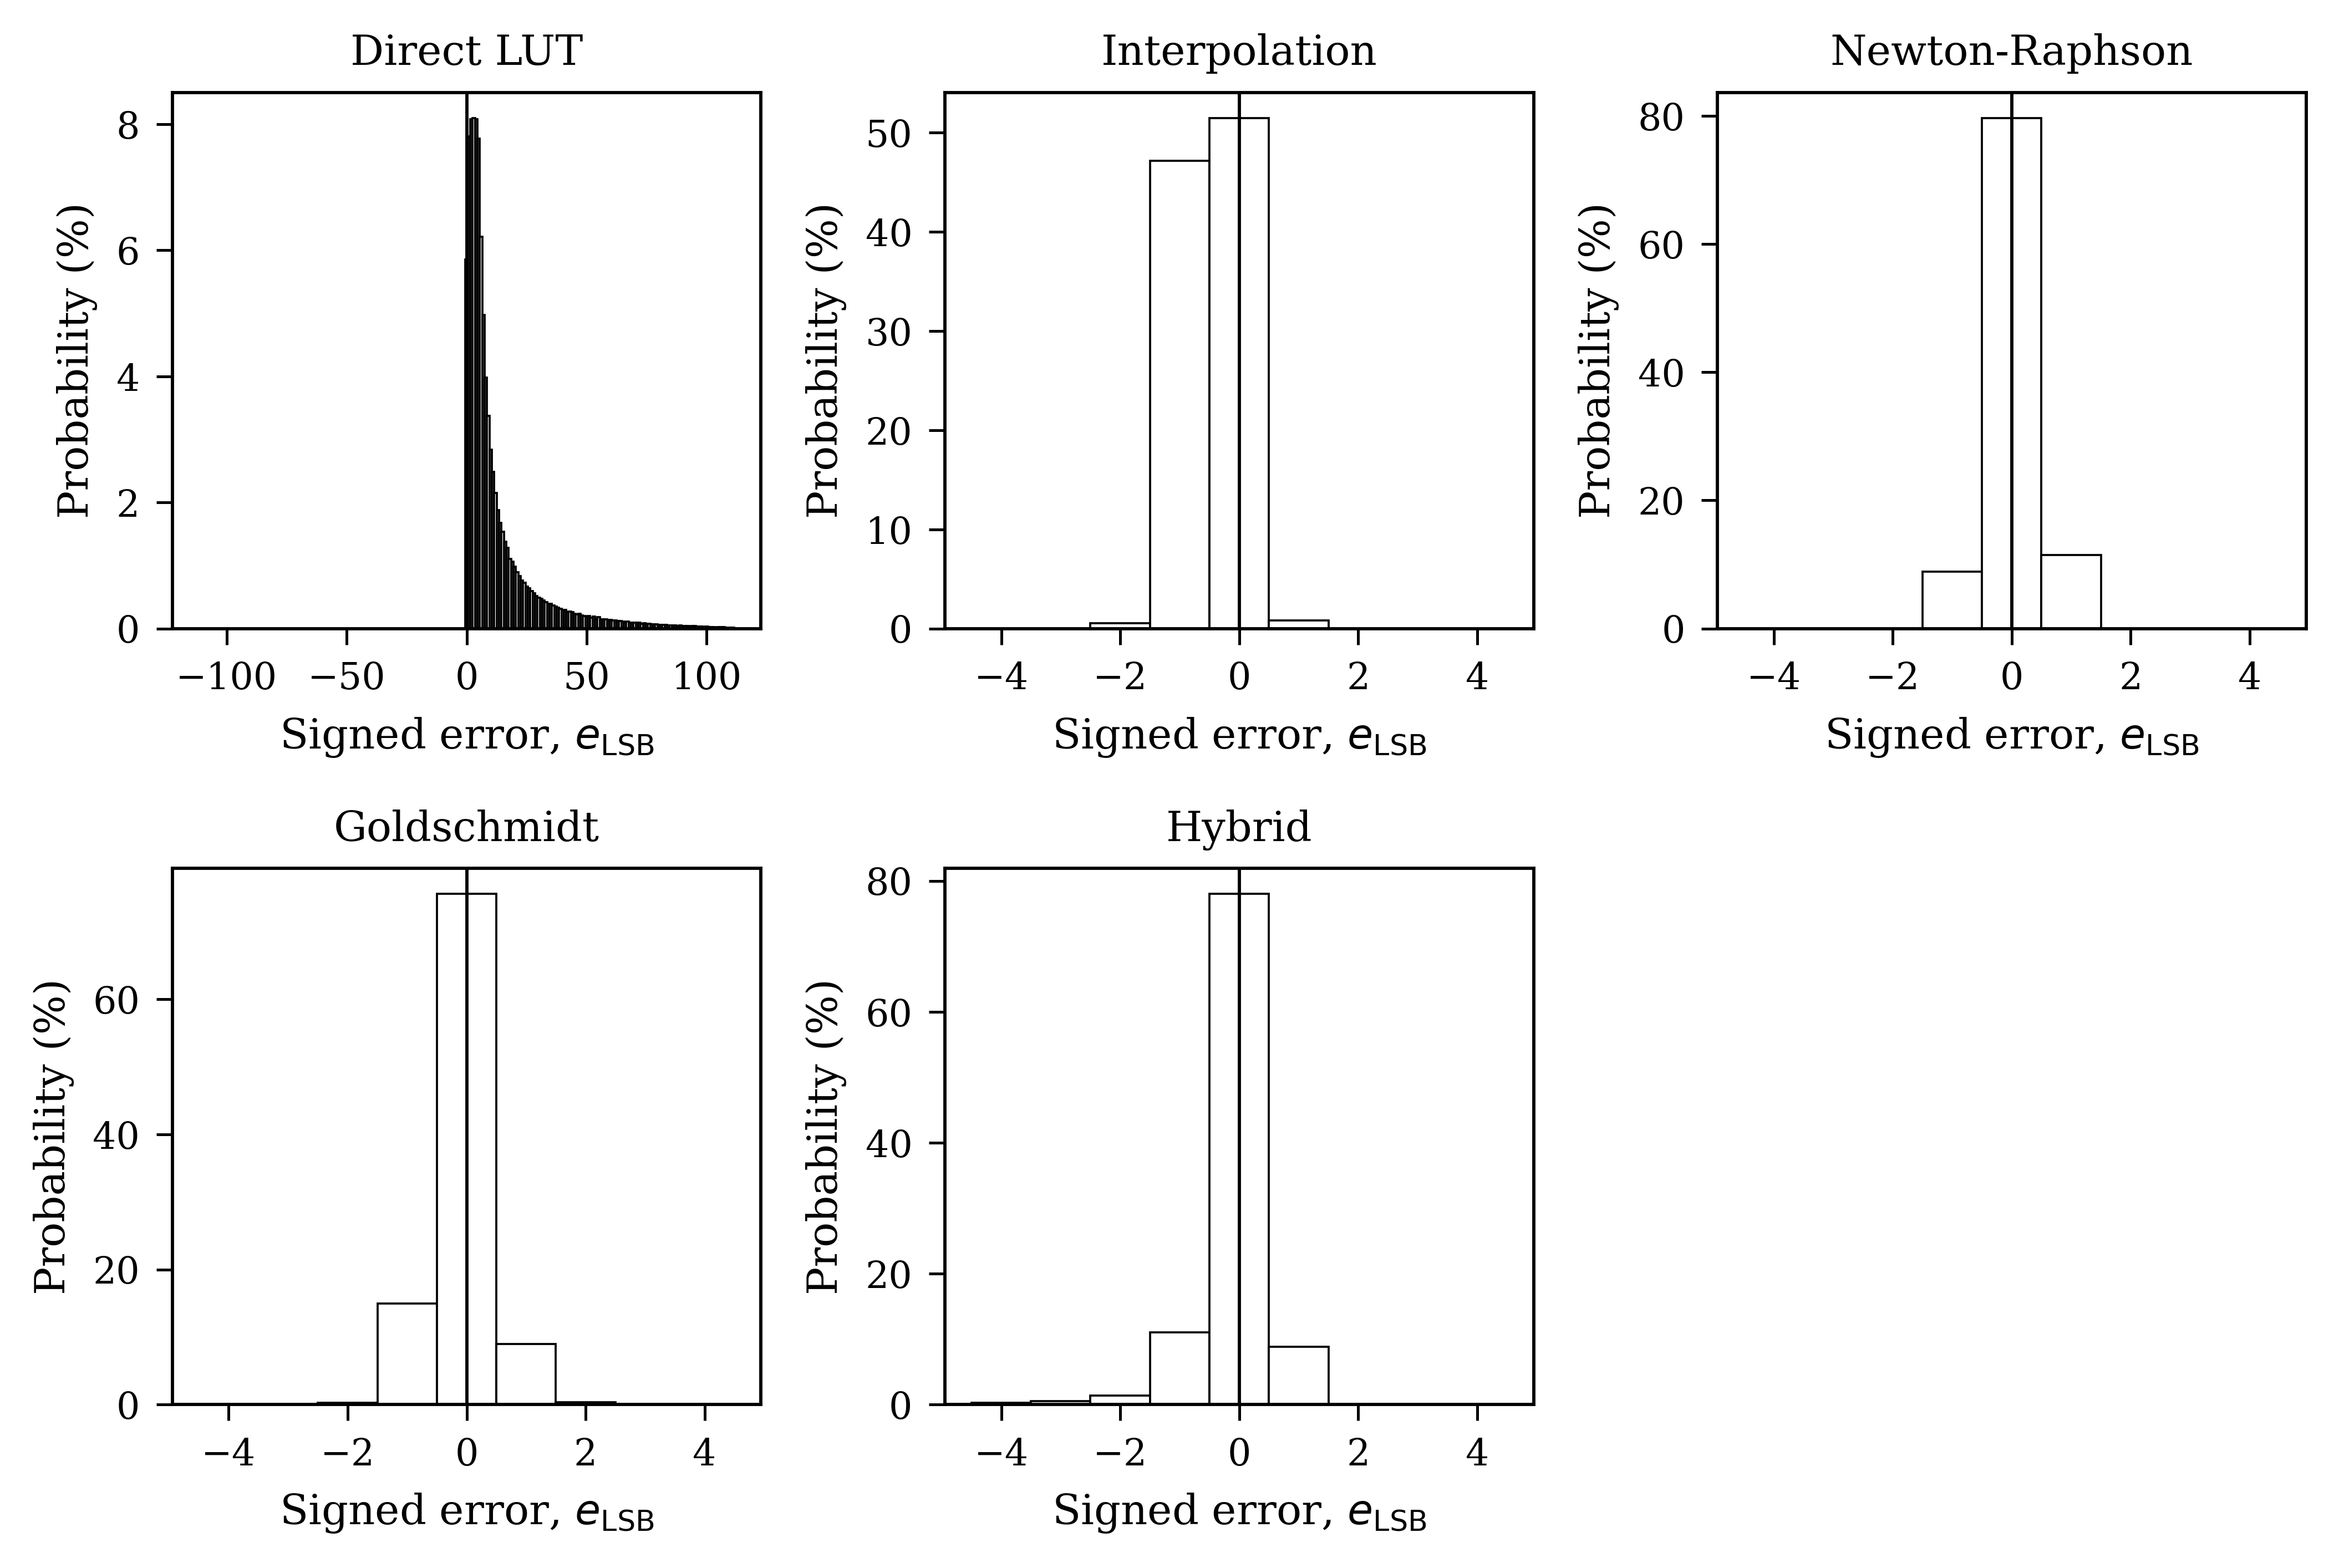
\includegraphics[width=\linewidth]{figures/q16_signederror.png}
\caption{Signed error distributions (error in LSB) by architecture, Q16.16.}
\Description{Overlaid histograms on a shared LSB axis. Direct LUT is the widest, with an RMSE of 20.75 LSB. The interpolation, Newton-Raphson, Goldschmidt and hybrid histograms all have RMSE between 0.45 and 0.71 LSB, so their errors sit within about one LSB of zero.}
\label{fig:errdist1616}
\end{figure}

\begin{figure}[H]
\centering
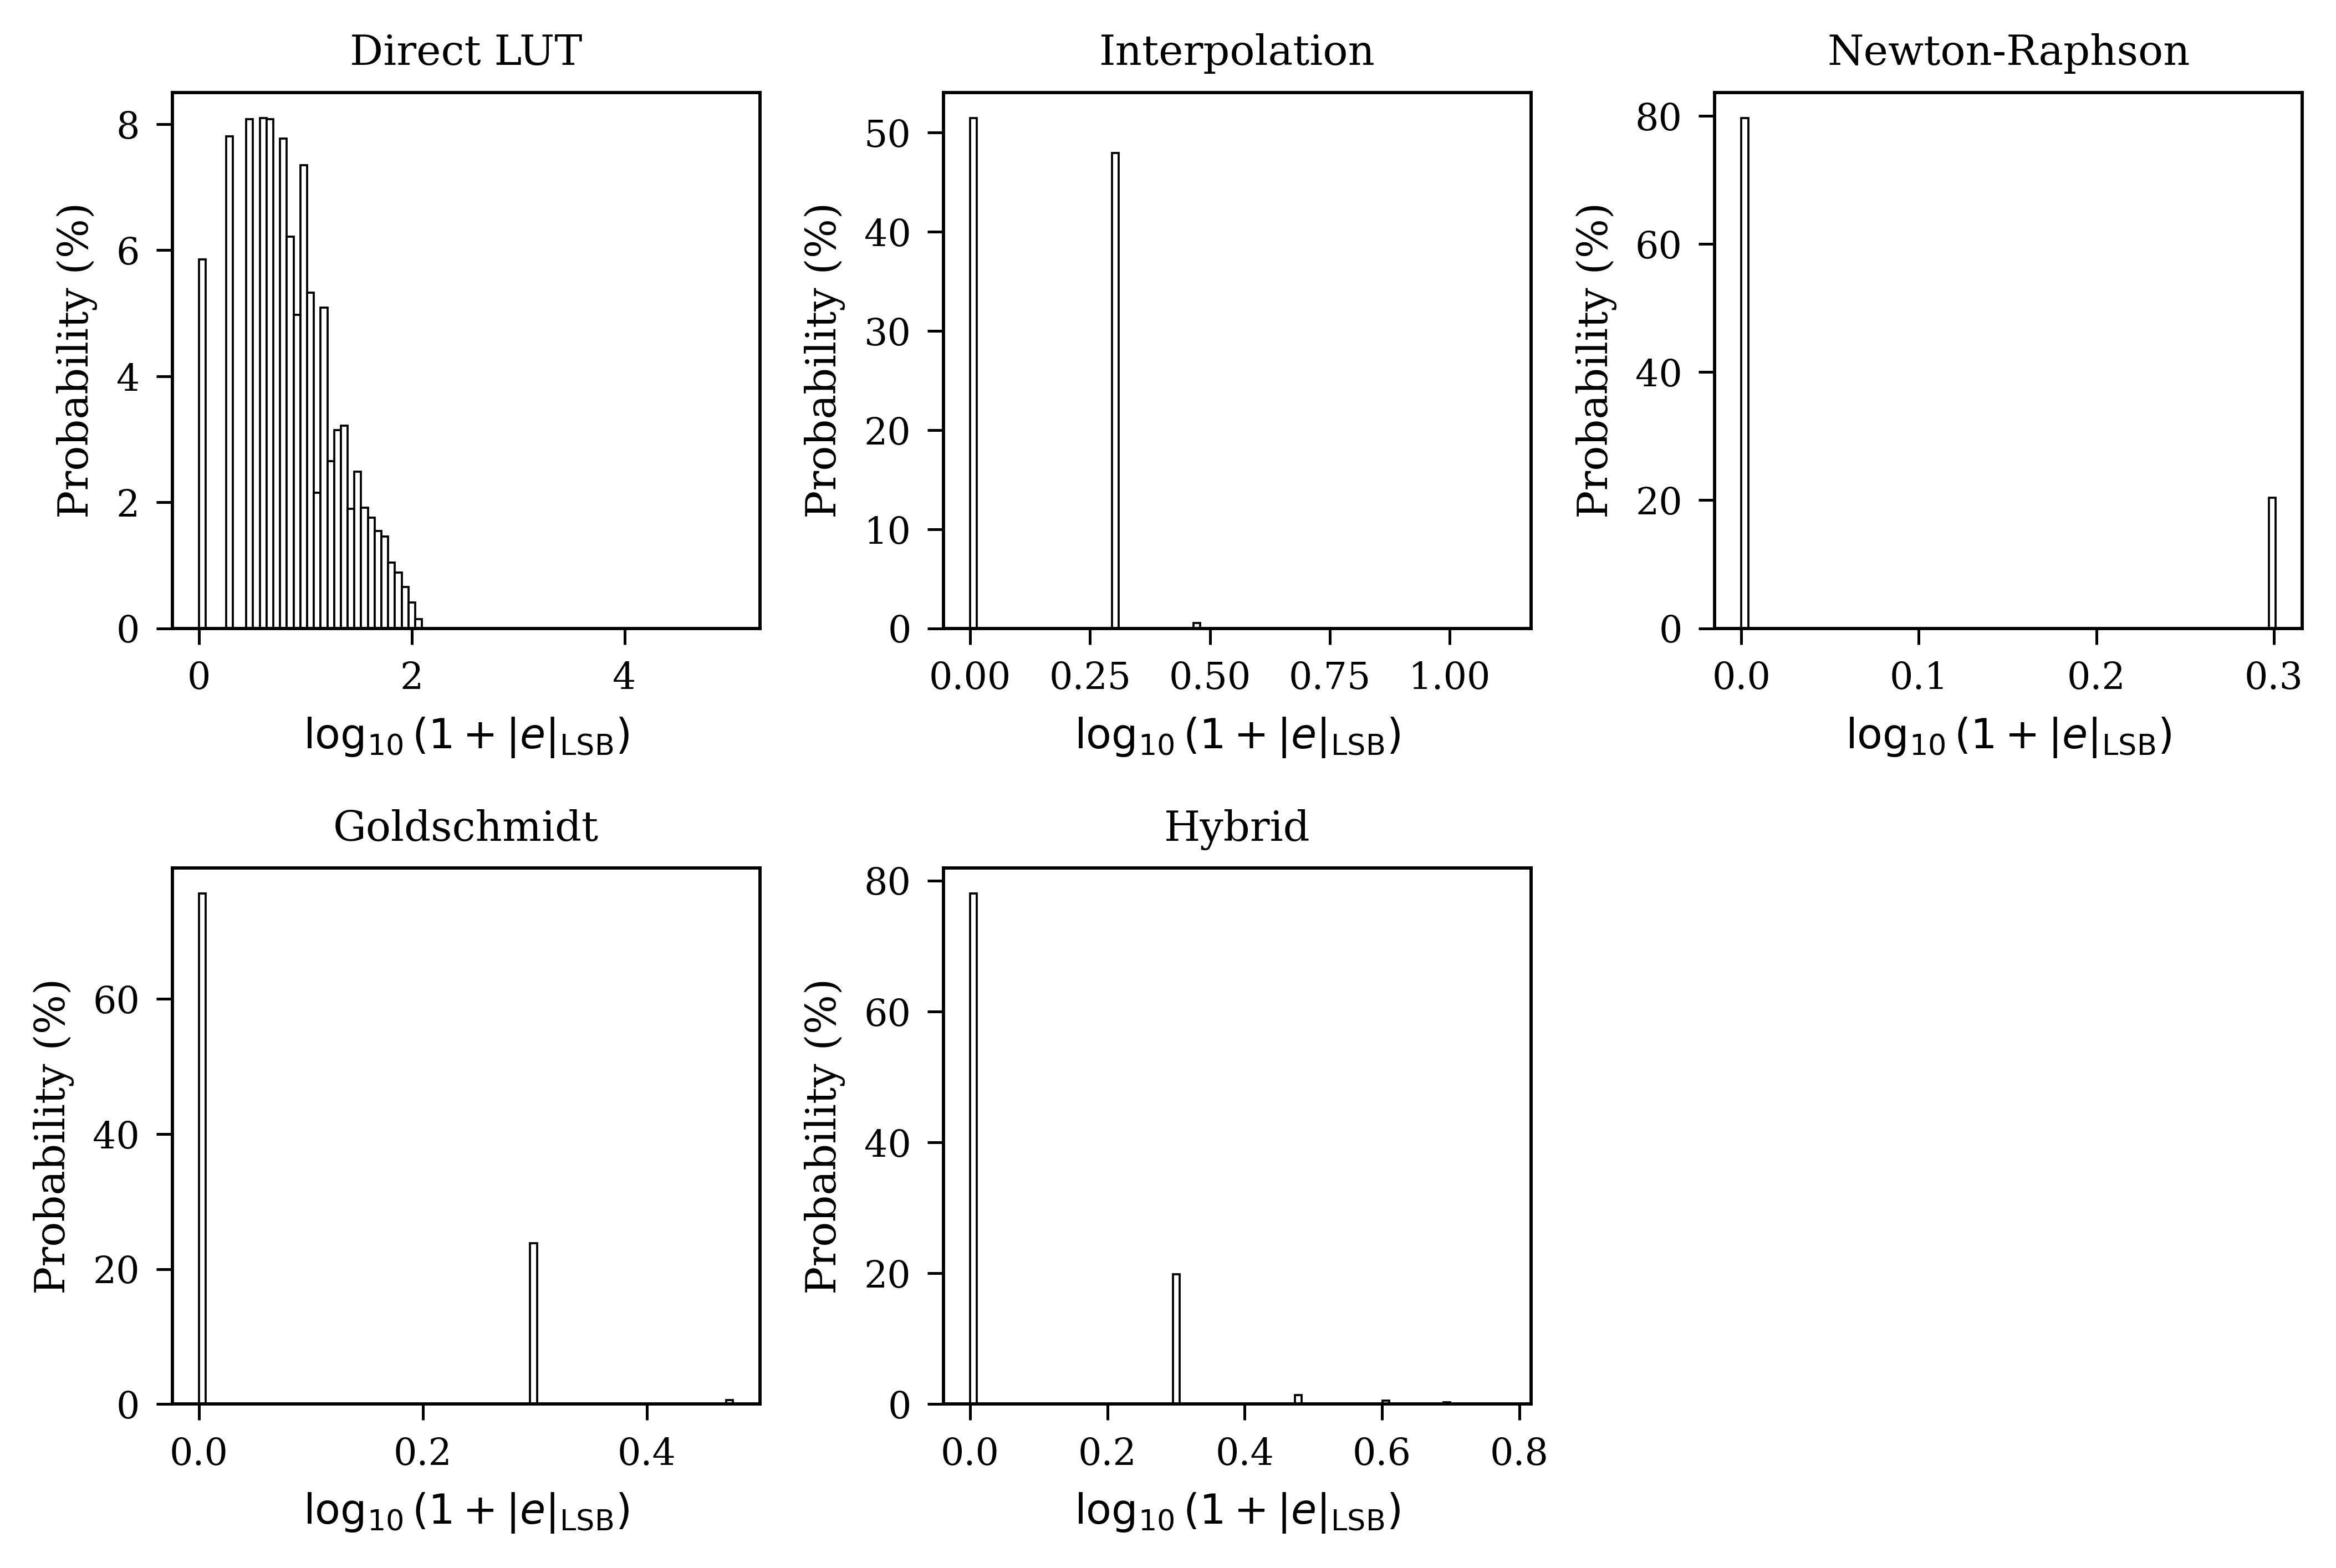
\includegraphics[width=\linewidth]{figures/q16_abserr.png}
\caption{Absolute error $|e|$ distributions by architecture, Q16.16 ($\log_{10}(1+|e|)$ scale).}
\Description{Overlaid histograms on a compressed horizontal axis. The largest observed absolute errors are 0.00189 for Direct LUT (about 124 LSB), 0.000183 for interpolation, 0.0000763 for the hybrid (about 5 LSB), 0.0000305 for Goldschmidt (about 2 LSB) and 0.0000153 for Newton-Raphson (1 LSB). Only the Direct LUT and interpolation histograms extend well beyond a few LSB.}
\label{fig:errdistlog1616}
\end{figure}

\begin{figure}[H]
\centering
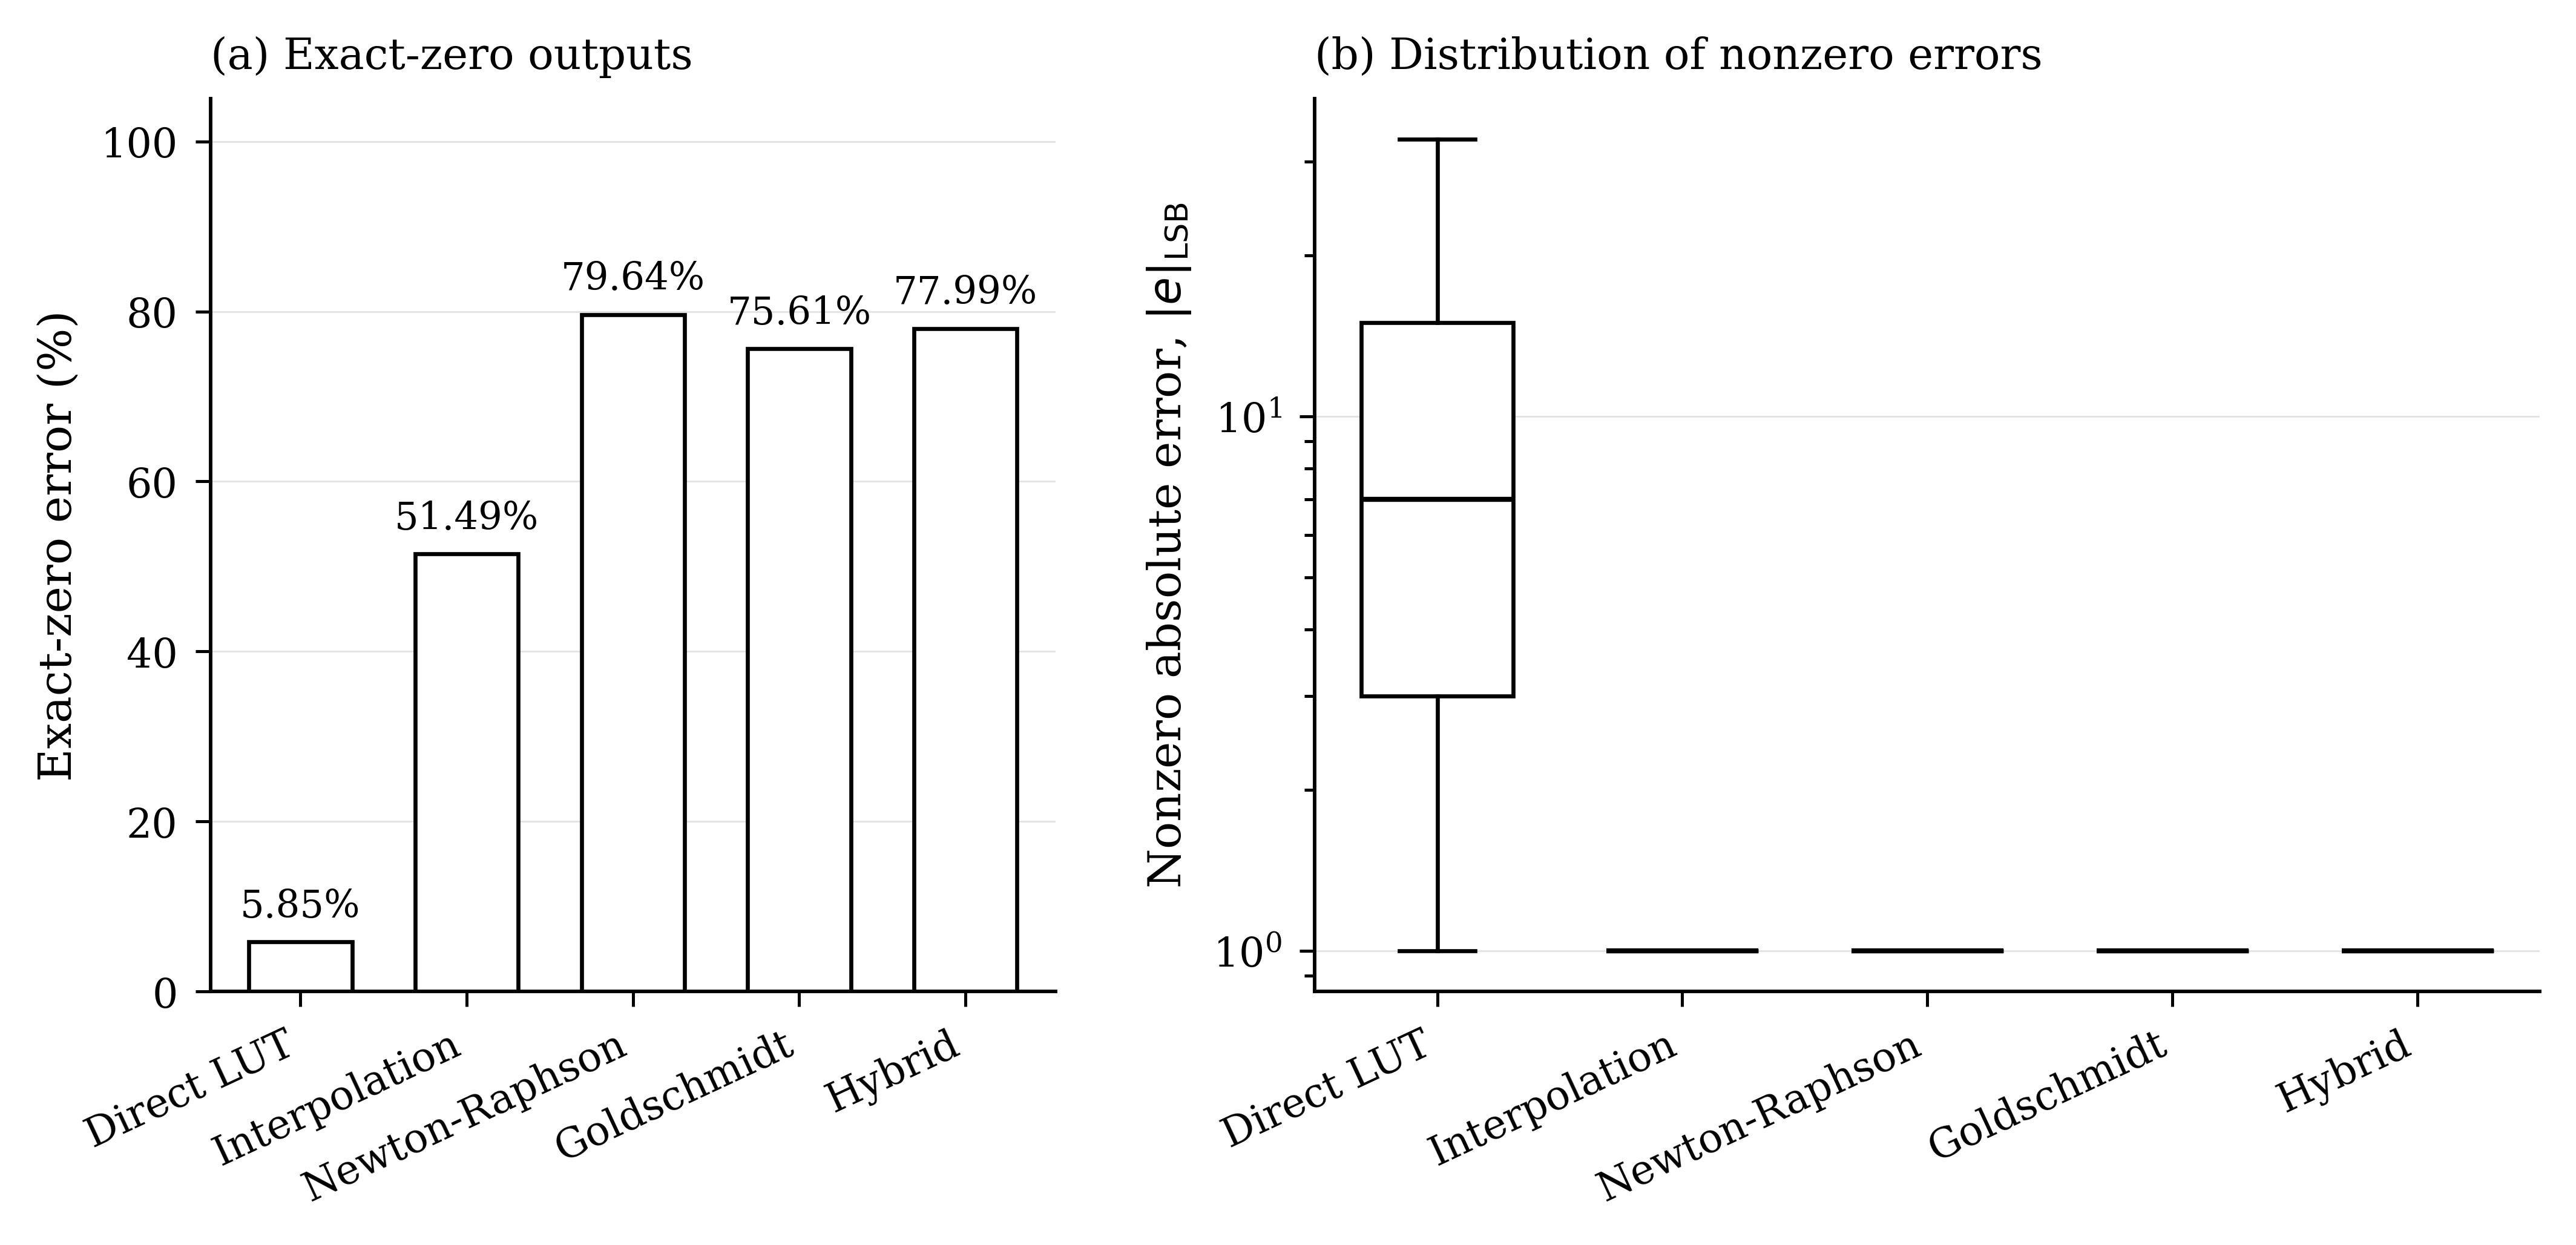
\includegraphics[width=\linewidth]{figures/q16_zeroerr.png}
\caption{Zero-LSB output fraction and distribution of nonzero signed errors (LSB) by architecture, Q16.16.}
\Description{Two views per architecture. Because the Newton-Raphson, Goldschmidt, hybrid and interpolation architectures have RMSE values of only 0.45 to 0.71 LSB, their nonzero errors are confined to a few LSB. Direct LUT has the widest spread of nonzero errors, reaching about 124 LSB at most.}
\label{fig:zerolsb1616}
\end{figure}

\begin{figure}[H]
\centering
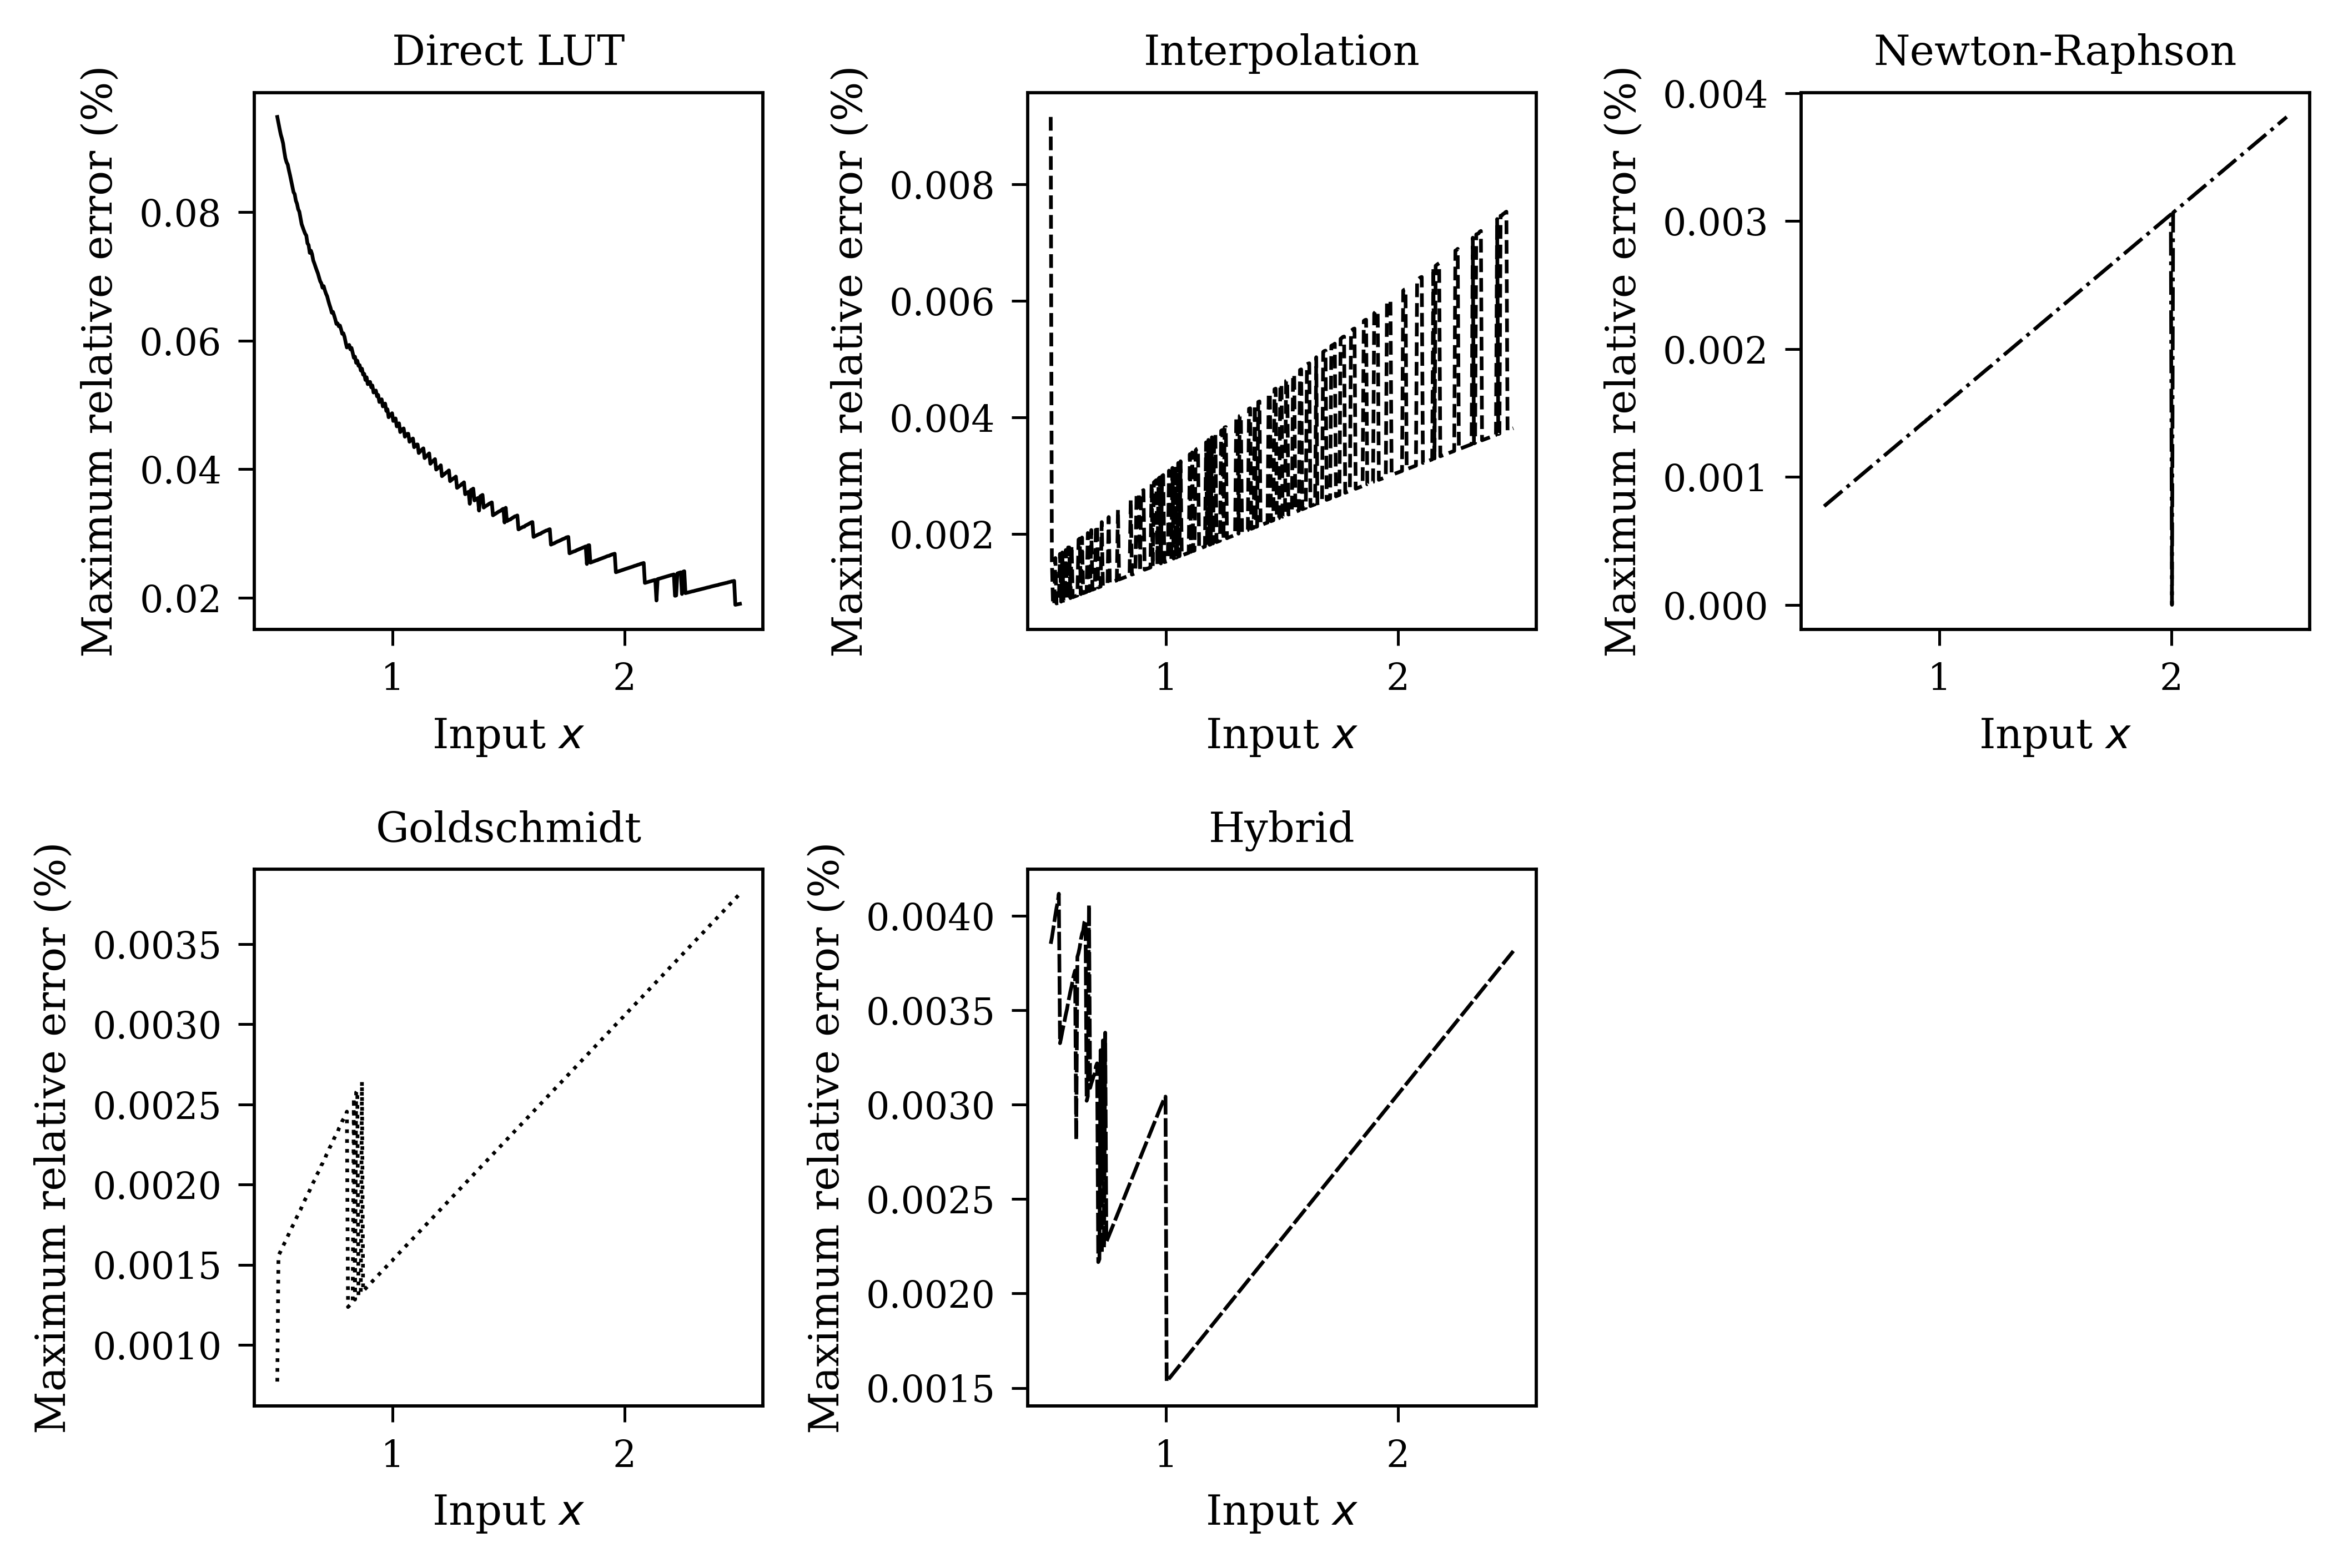
\includegraphics[width=0.85\linewidth]{figures/q16_relerr.png}
\caption{Maximum relative error (\%) as a function of input value $x$, by architecture, Q16.16.}
\Description{Line plot of relative error against x from 0.5 to 2.5. Direct LUT is highest, peaking near 0.095 percent, followed by interpolation near 0.0092 percent. The hybrid, Newton-Raphson and Goldschmidt curves are close together at the bottom, with maxima of about 0.0041, 0.0038 and 0.0038 percent.}
\label{fig:maxrelerr1616}
\end{figure}

\begin{figure}[H]
\centering
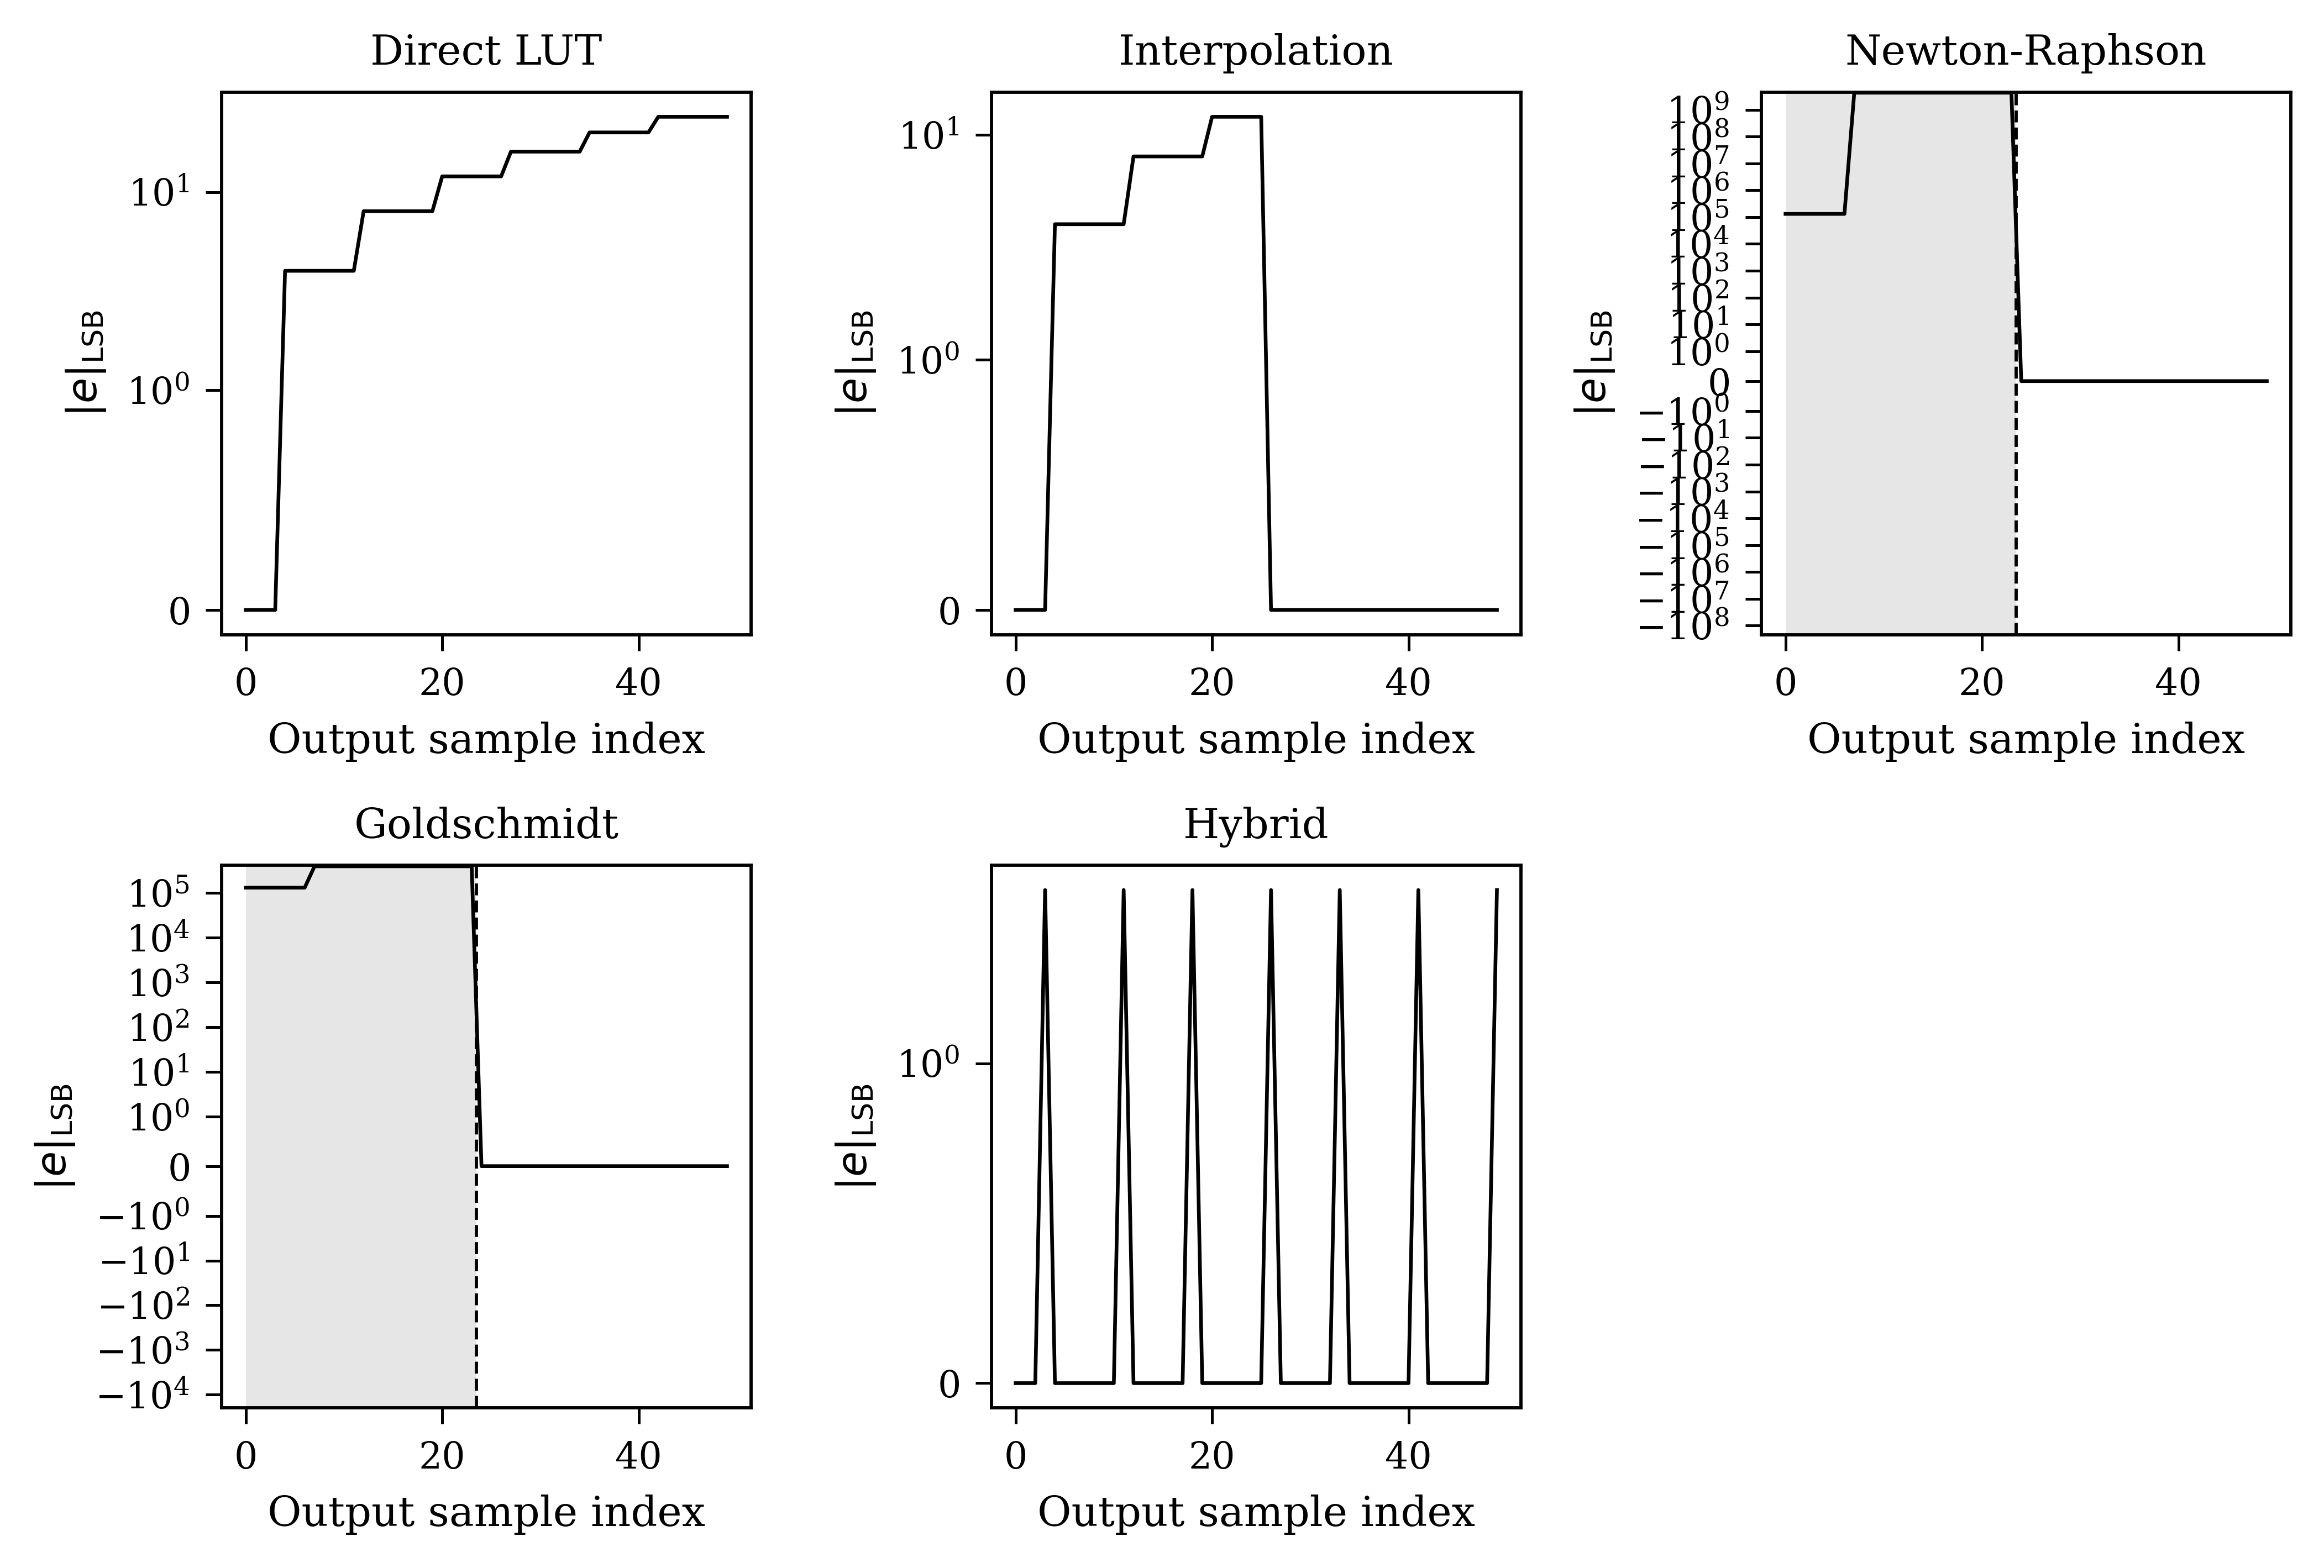
\includegraphics[width=0.85\linewidth]{figures/q16_pipelinewarmup.png}
\caption{Output error during the pipeline warm-up transient by architecture (shaded region: pipeline fill period), Q16.16.}
\Description{Time-series traces of output error over the first samples. The shaded fill period is 3 samples for Direct LUT, 16 for interpolation, 40 for the hybrid, 54 for Goldschmidt and 69 for Newton-Raphson. Outputs inside the shaded region are not valid results.}
\label{fig:warmup1616}
\end{figure}

\begin{figure}[H]
\centering
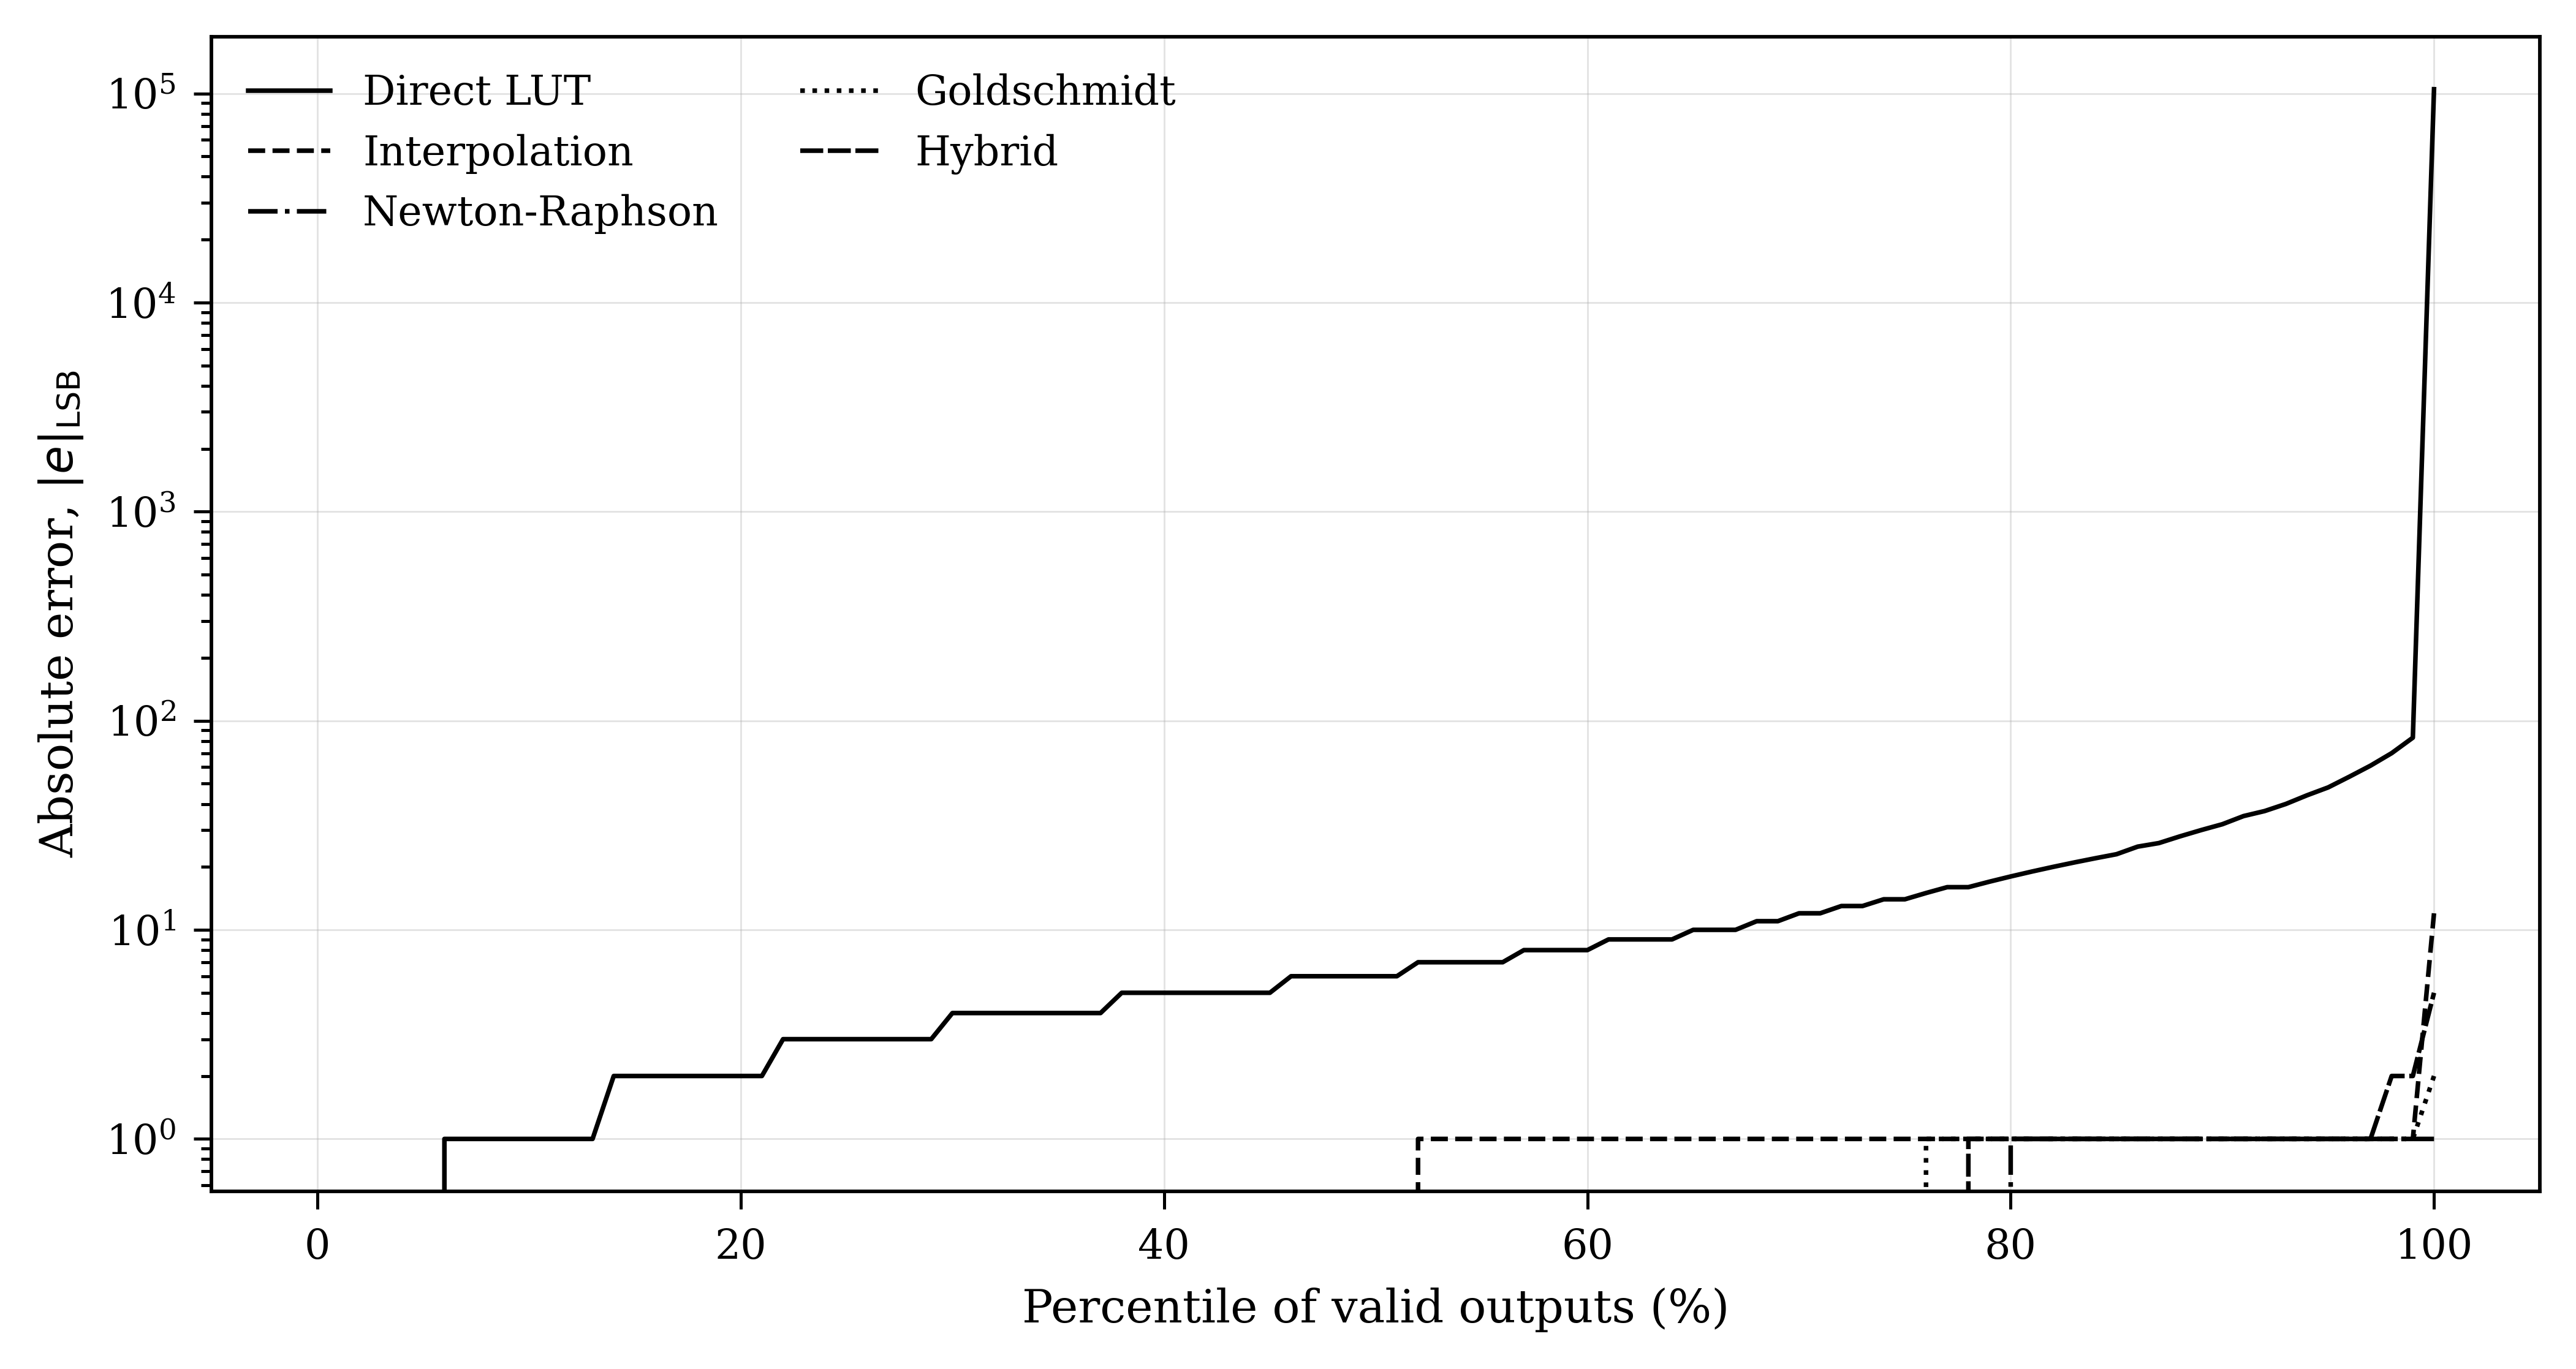
\includegraphics[width=0.9\linewidth]{figures/q16_errorpercentile.png}
\caption{Absolute error (real-valued) as a function of output percentile, all architectures, Q16.16.}
\Description{Curves of absolute error against output percentile. The maximum absolute errors are 0.00189 for Direct LUT, 0.000183 for interpolation, 0.0000763 for the hybrid, 0.0000305 for Goldschmidt and 0.0000153 for Newton-Raphson. The last three curves lie close together at the bottom of the plot.}
\label{fig:percentile1616}
\end{figure}

\subsection{Power and Energy}
\label{sec:power}

Table~\ref{tab:power} and Fig.~\ref{fig:summary} report dynamic, static, and total power estimates together with the derived energy per operation (Eq.~(\ref{eq:energyop})) for all ten architecture/format combinations. The highest total power estimates (0.458 to 0.483~W) are observed for the two multiplier-intensive iterative architectures, which also exhibit the highest DSP and flip-flop utilization; combined with their long pipeline latency, they also have the highest energy per operation (1.167 to 1.219~nJ/op). In Q8.24 the Direct LUT architecture has the lowest energy per operation (0.346~nJ/op), reflecting both its minimal dynamic power estimate and its short pipeline; in Q16.16 the lowest value belongs to LUT-Interpolation (0.379~nJ/op, against 0.412~nJ/op for Direct LUT). Static power estimates vary only slightly (0.091 to 0.092~W) across the ten configurations.

\begin{table}[H]
\caption{Post-Implementation Power Estimates and Derived Energy}
\label{tab:power}
\begin{tabular}{@{}llrrrr@{}}
\toprule
\textbf{Architecture} & \textbf{Format} & \textbf{Dynamic P (W)} & \textbf{Static P (W)} & \textbf{Total P (W)} & \textbf{Energy/op (nJ)} \\
\midrule
Direct LUT & Q8.24 & 0.045 & 0.091 & 0.136 & 0.346 \\
Direct LUT & Q16.16 & 0.122 & 0.092 & 0.214 & 0.412 \\
LUT-Interpolation & Q8.24 & 0.083 & 0.091 & 0.174 & 0.405 \\
LUT-Interpolation & Q16.16 & 0.070 & 0.091 & 0.161 & 0.379 \\
Newton-Raphson & Q8.24 & 0.383 & 0.092 & 0.475 & 1.190 \\
Newton-Raphson & Q16.16 & 0.366 & 0.092 & 0.458 & 1.167 \\
Goldschmidt & Q8.24 & 0.391 & 0.092 & 0.483 & 1.219 \\
Goldschmidt & Q16.16 & 0.385 & 0.092 & 0.477 & 1.208 \\
Hybrid & Q8.24 & 0.227 & 0.092 & 0.319 & 1.009 \\
Hybrid & Q16.16 & 0.228 & 0.092 & 0.320 & 1.049 \\
\bottomrule
\end{tabular}
\end{table}

\subsection{Cross-Format Comparison}
\label{sec:crossformat}

Figs.~\ref{fig:cross_fmax}-\ref{fig:cross_full} directly compare Q8.24 and Q16.16 across achieved $F_{\max}$ and latency, slice LUT/DSP resource usage, total power and energy per operation, and full four-metric resource utilization, respectively. Two cross-format effects are evident. First, Direct LUT achieves markedly higher $F_{\max}$ in Q16.16 than in Q8.24, increasing from 392.8~MHz to 519.2~MHz, whereas LUT-Interpolation is essentially unchanged (429.7~MHz versus 424.5~MHz). This difference is consistent with the narrower output representation and the resulting implementation of the BRAM/output datapath, although the exact timing improvement depends on the post-implementation critical paths. Newton-Raphson, Goldschmidt, and Hybrid likewise show comparatively small $F_{\max}$ differences between the two formats, reflecting the greater influence of their pipelined arithmetic datapaths on the achieved timing.

Second, the iterative and hybrid architectures exhibit substantially different accuracy behavior across the two formats. Newton-Raphson and Goldschmidt, both seeded from 8-bit-address coarse lookup tables, show substantially higher maximum relative error in Q16.16 than in Q8.24, by approximately two orders of magnitude. The Hybrid architecture, which uses a 9-bit-address interpolated seed followed by a Newton-Raphson refinement, also shows a higher maximum relative error in Q16.16. This behavior is consistent with the reduced fractional precision of Q16.16, which provides fewer bits for representing intermediate and final correction terms throughout the fixed-point refinement process.

These results illustrate that the effect of fixed-point format extends beyond numerical representation alone and influences the measured timing and accuracy characteristics of the architectures. Consequently, the relative trade-offs among accuracy, latency, and energy depend on both the reciprocal algorithm and the fixed-point format used by the surrounding system.

\begin{figure}[H]
\centering
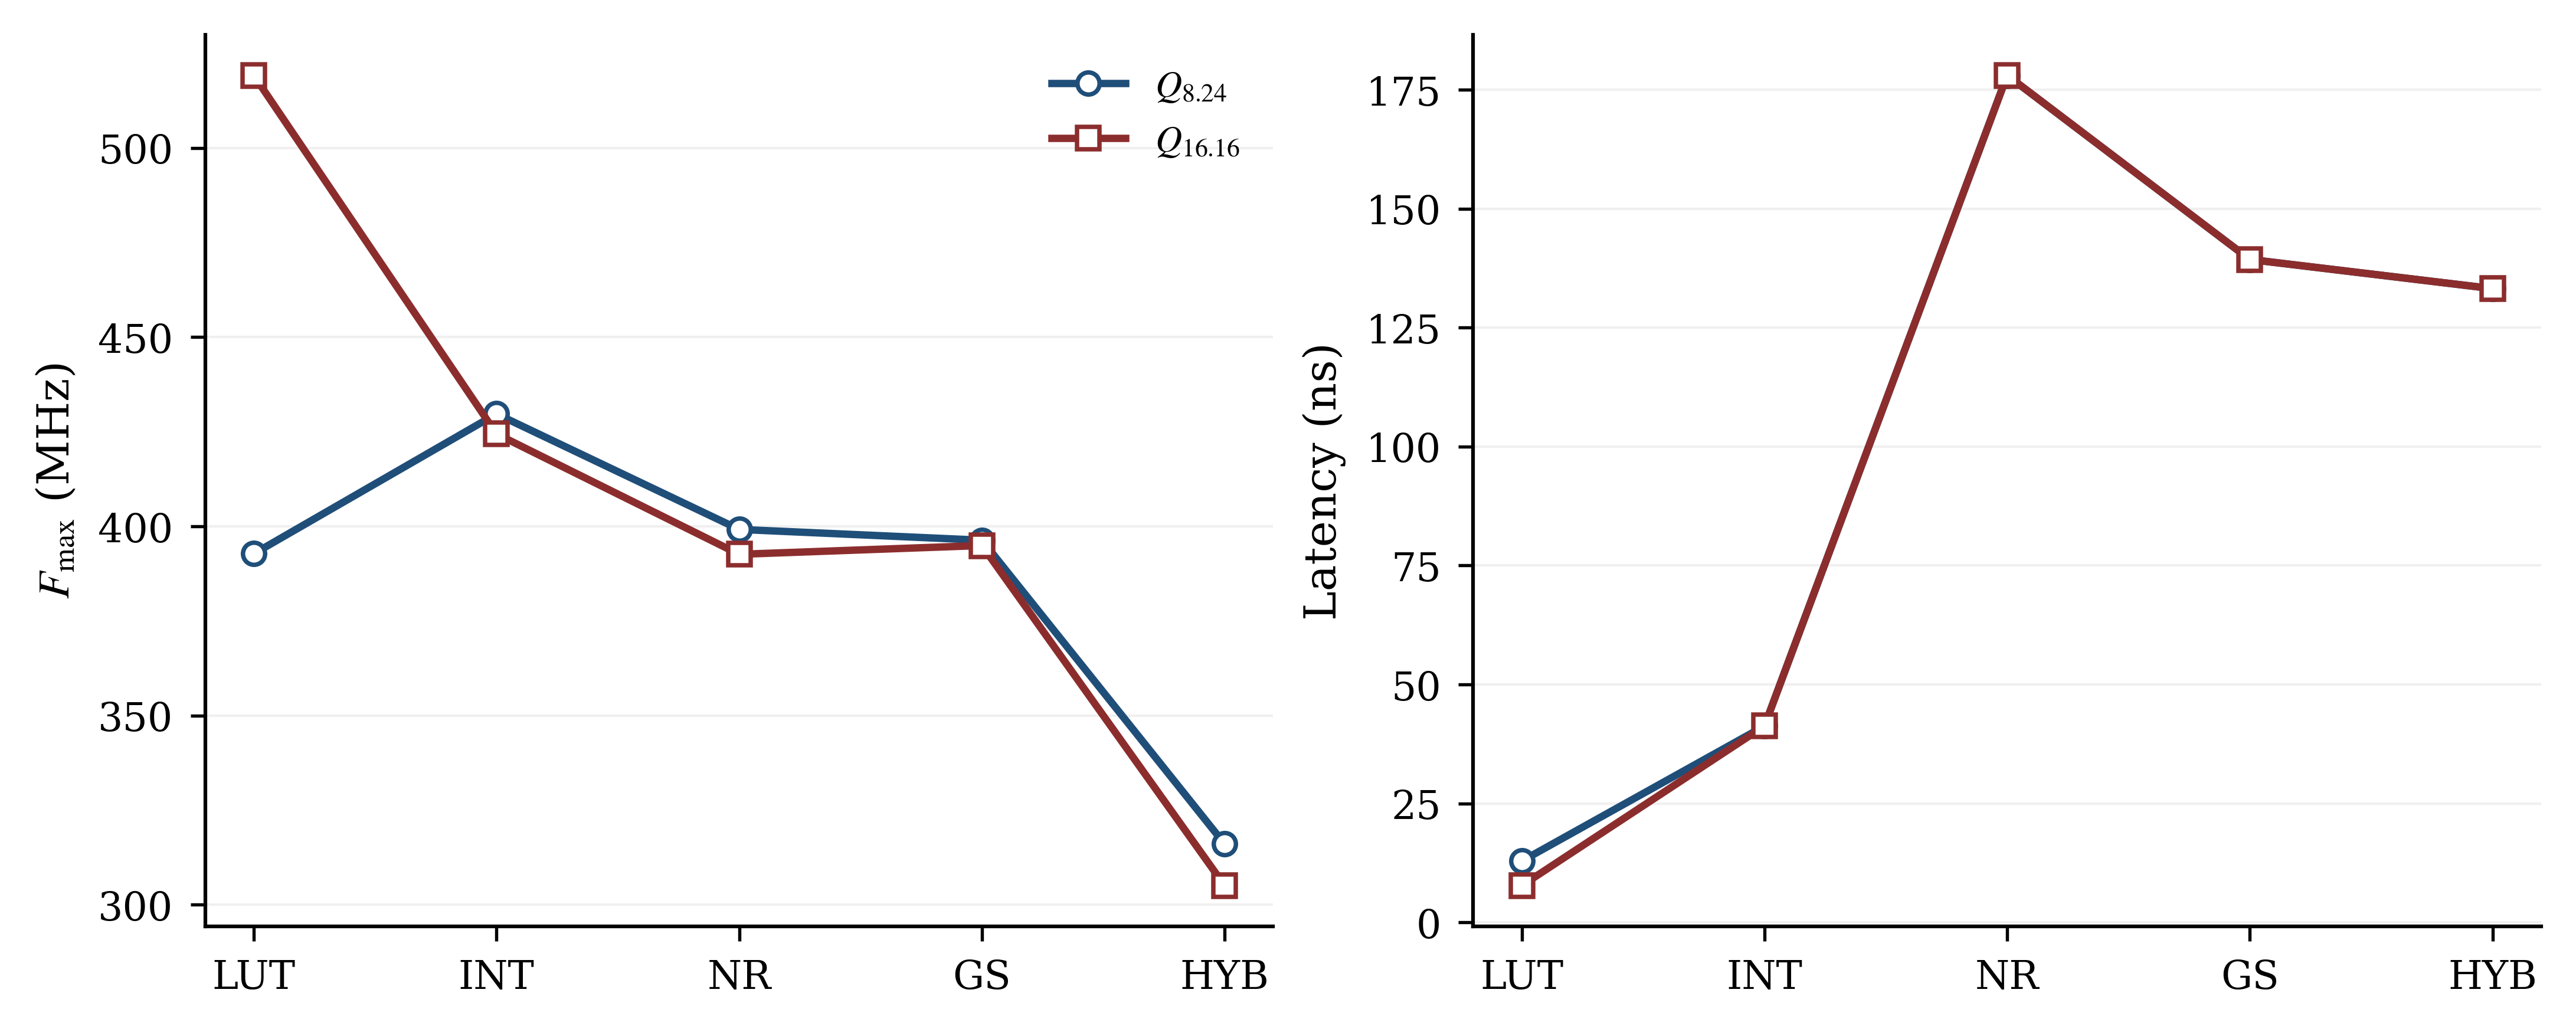
\includegraphics[width=\linewidth]{figures/fmax_latency_plot.png}
\caption{Achieved $F_{\max}$ (MHz) and latency (ns) by architecture, Q8.24 versus Q16.16.}
\Description{Paired bars for the two formats. F max in Q8.24 versus Q16.16 is 392.77 versus 519.21 MHz for Direct LUT, 429.74 versus 424.45 for interpolation, 399.20 versus 392.62 for Newton-Raphson, 396.35 versus 394.94 for Goldschmidt and 316.06 versus 305.06 for the hybrid. Latency is identical across formats except for Direct LUT (12.90 versus 7.74 ns), and rises from 41.28 ns for interpolation to 178.02 ns for Newton-Raphson.}
\label{fig:cross_fmax}
\end{figure}

\begin{figure}[H]
\centering
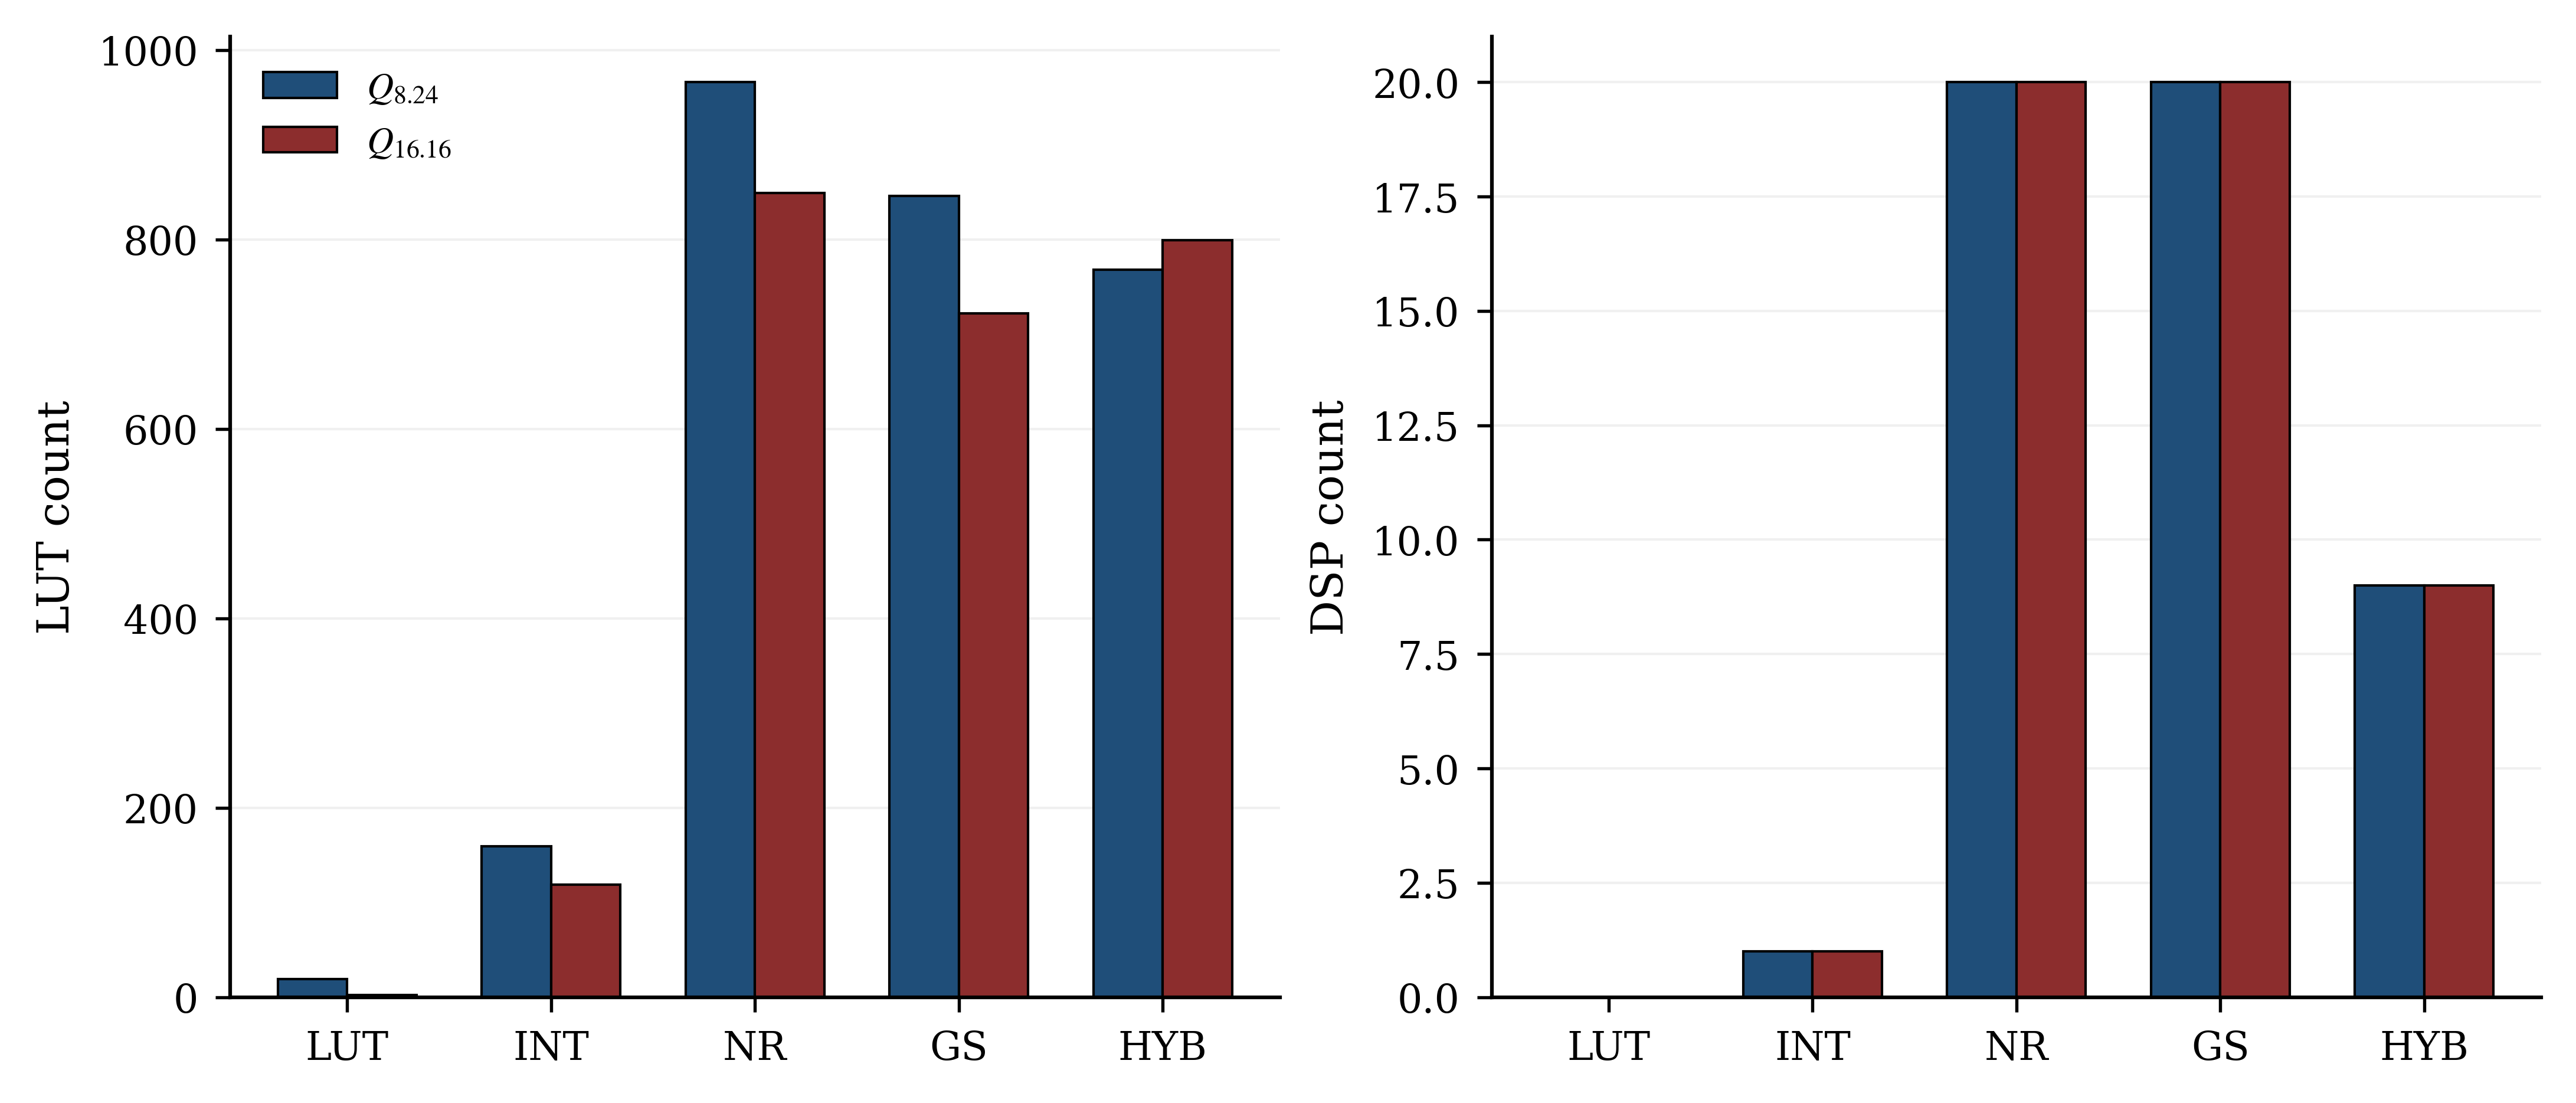
\includegraphics[width=\linewidth]{figures/lut_dsp_bar_plot.png}
\caption{Slice LUT and DSP utilization (resource counts) by architecture, Q8.24 versus Q16.16.}
\Description{Paired bars for the two formats. LUT counts in Q8.24 versus Q16.16 are 19 versus 2 for Direct LUT, 159 versus 119 for interpolation, 966 versus 849 for Newton-Raphson, 846 versus 722 for Goldschmidt and 768 versus 799 for the hybrid. DSP counts are 0, 1, 20, 20 and 9 in the same order, identical in both formats.}
\label{fig:cross_lutdsp}
\end{figure}

\begin{figure}[H]
\centering
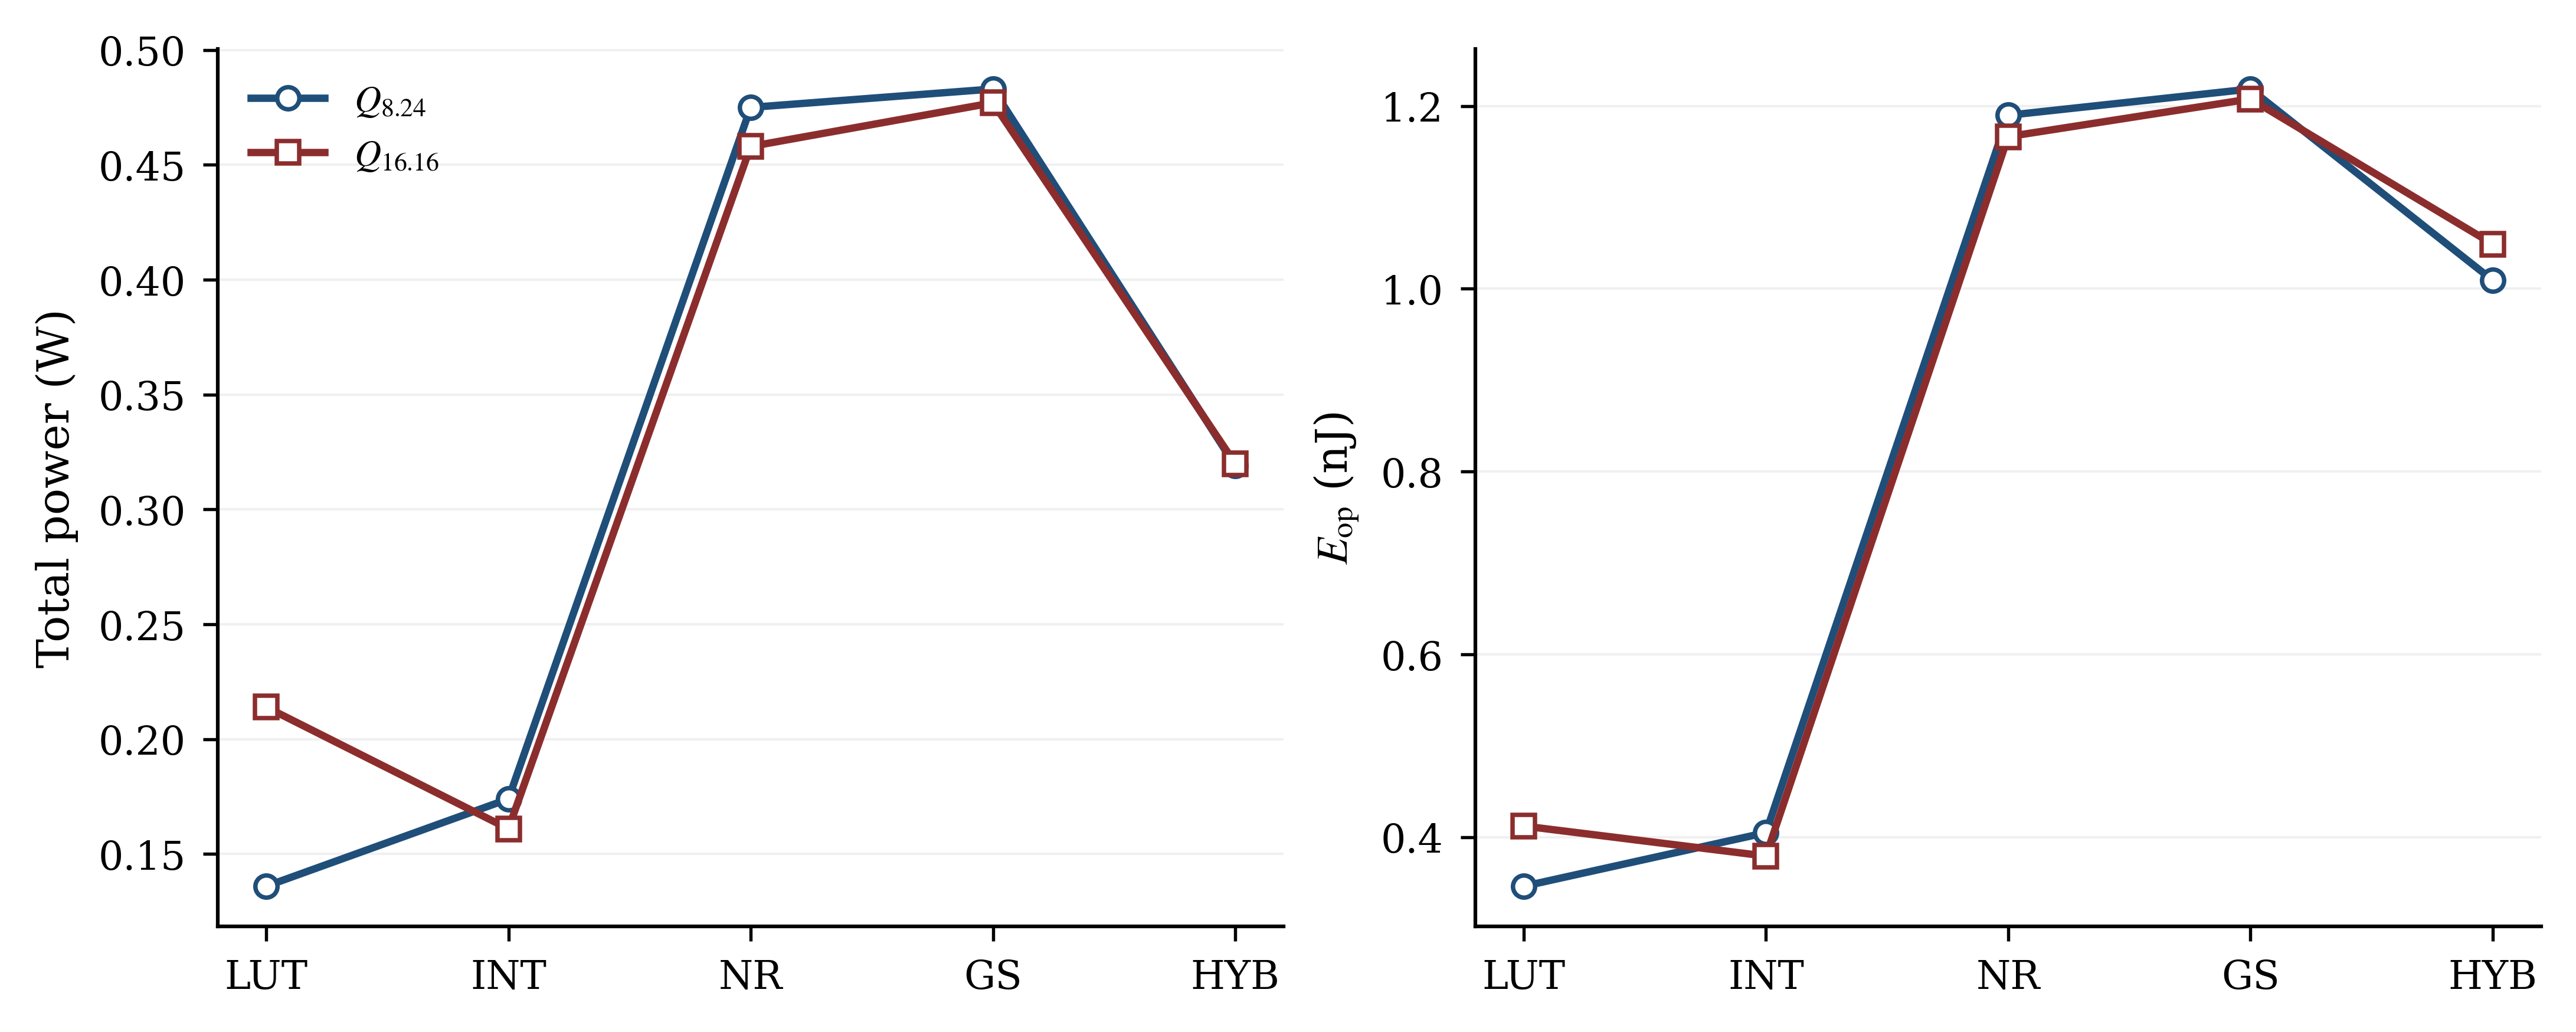
\includegraphics[width=\linewidth]{figures/power_energy_plot.png}
\caption{Total power (W) and energy per operation (nJ/op) by architecture, Q8.24 versus Q16.16.}
\Description{Paired bars for the two formats. Total power estimates in Q8.24 versus Q16.16 are 0.136 versus 0.214 W for Direct LUT, 0.174 versus 0.161 for interpolation, 0.475 versus 0.458 for Newton-Raphson, 0.483 versus 0.477 for Goldschmidt and 0.319 versus 0.320 for the hybrid. Energy per operation is 0.346 versus 0.412 nJ, 0.405 versus 0.379, 1.190 versus 1.167, 1.219 versus 1.208 and 1.009 versus 1.049 in the same order.}
\label{fig:cross_power}
\end{figure}

\begin{figure}[H]
\centering
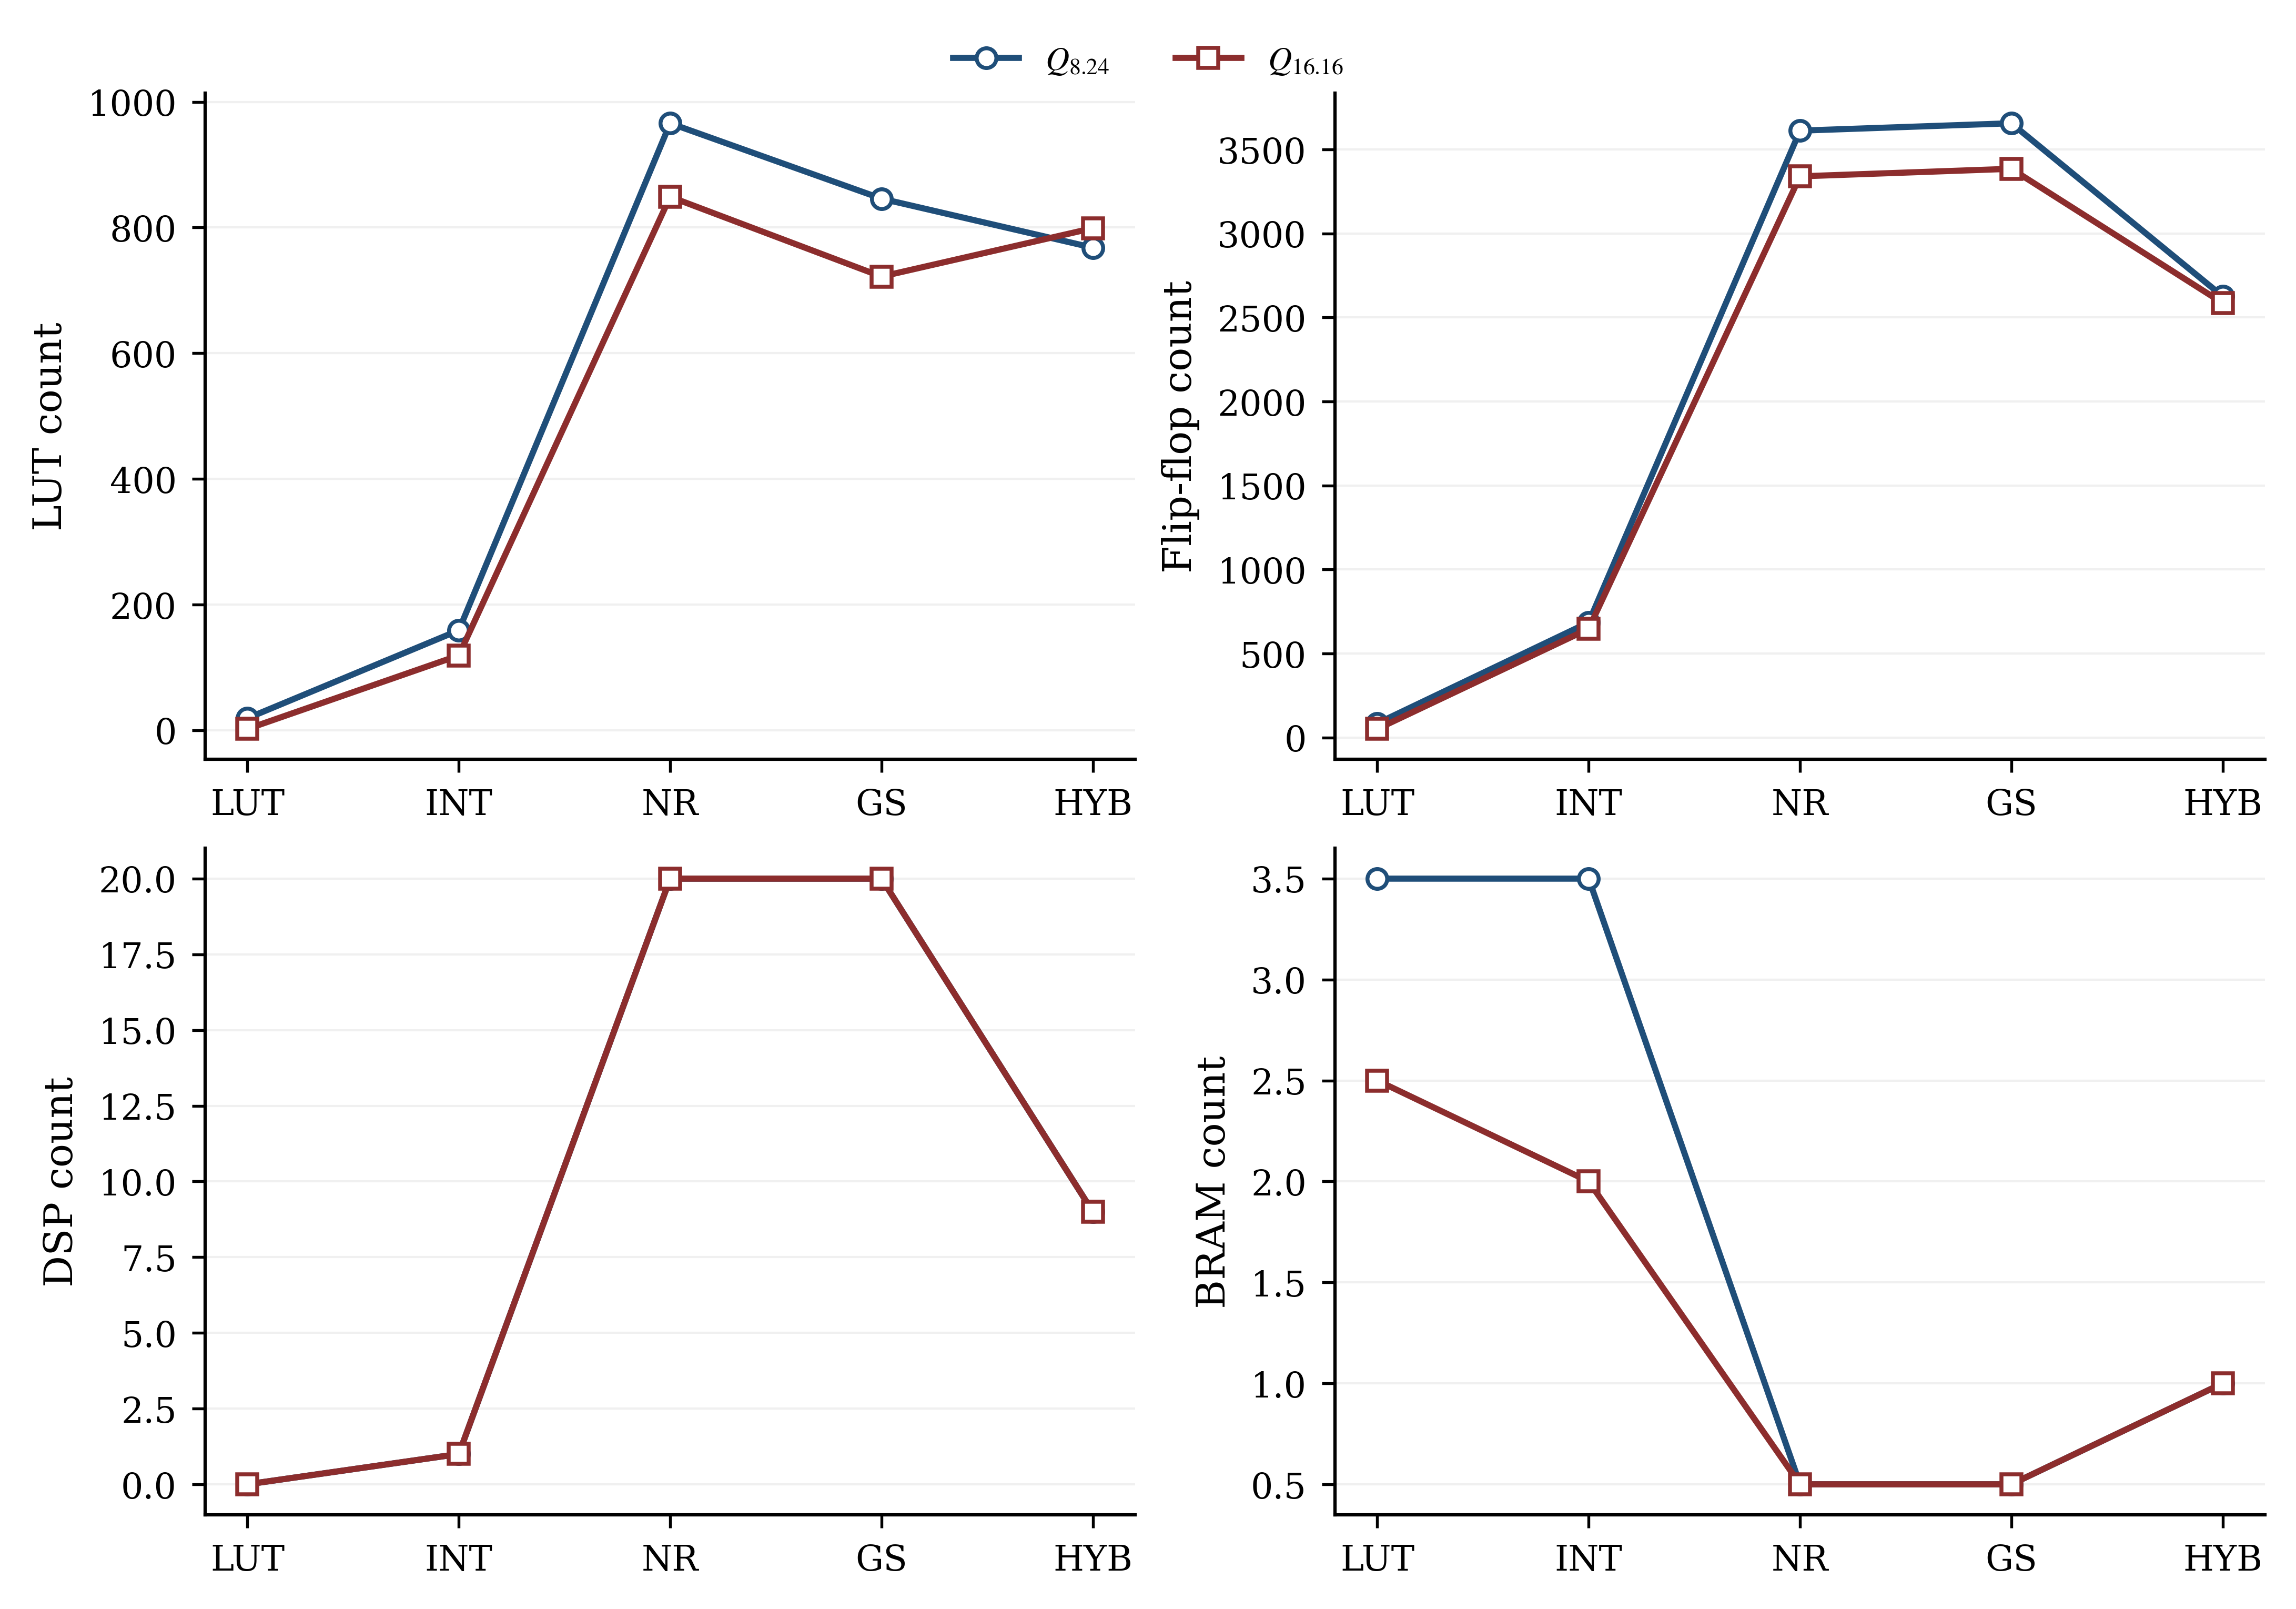
\includegraphics[width=\linewidth]{figures/resources_plot.png}
\caption{Full resource utilization (slice LUT, FF, DSP, BRAM counts) by architecture, Q8.24 versus Q16.16.}
\Description{Paired bars for the two formats covering four resources. Flip-flop counts are 84 and 51 for Direct LUT, 685 and 647 for interpolation, 3612 and 3340 for Newton-Raphson, 3656 and 3385 for Goldschmidt, and 2626 and 2586 for the hybrid. BRAM usage is 3.5 and 2.5 for Direct LUT, 3.5 and 2.0 for interpolation, 0.5 for both iterative architectures, and 1.0 for the hybrid. LUT and DSP counts match the previous cross-format figure.}
\label{fig:cross_full}
\end{figure}

\section{Pareto Trade-off Analysis}
\label{sec:pareto}

\subsection{Pareto Formulation}
\label{sec:paretoform}

The results of Section~\ref{sec:results} show that no single architecture dominates the others across every metric of interest. The relative ordering depends on the fixed-point format and the metric considered: the iterative architectures provide substantially lower numerical error than the table-based approaches, but generally incur higher latency and energy per operation, whereas the Direct LUT architecture provides the shortest latency with low energy per operation at the cost of higher approximation error. To characterize these trade-offs rigorously rather than anecdotally, this section applies a three-objective Pareto analysis over maximum relative error, latency, and energy per operation:
\begin{equation}
\text{minimize} \; \{ E_{\max,rel},\, L_{ns},\, E_{op} \}
\label{eq:paretomin}
\end{equation}
Hardware resource utilization (slice LUT, FF, DSP, BRAM) is deliberately reported separately (Table~\ref{tab:resources}) rather than folded into the Pareto objective set above. A composite resource metric would require assigning relative weights across four resource types with different device-level scarcity and cost characteristics (e.g., BRAM versus DSP), and any such weighting would introduce a design choice into what is intended to be an objective, data-driven comparison; a design's resource cost is instead read directly from Table~\ref{tab:resources} alongside its position on the Pareto front. Given this three-objective formulation, an architecture $A$ is said to dominate an architecture $B$ if $A$ is no worse than $B$ on all three objectives and strictly better on at least one:
\begin{equation}
A \succ B \iff \left(\forall k \in \{E_{rel}, L, E_{op}\} : A_k \le B_k\right) \land \left(\exists k : A_k < B_k\right)
\label{eq:dominance}
\end{equation}
An architecture is Pareto-optimal (non-dominated) if no other evaluated architecture dominates it under this relation. Energy-delay product (EDP $= E_{op} \times L_{ns}$) is computed separately as a secondary, derived metric (Section~\ref{sec:edp}) rather than substituted for latency and energy as a combined objective, since two architectures with identical EDP can have substantially different individual energy and latency characteristics that matter for system-level integration (e.g., a hard real-time latency budget versus a battery energy budget), and collapsing the two into one number would discard that distinction.

\subsection{Pareto Fronts}

Fig.~\ref{fig:paretofront} plots each architecture's position in the latency-energy plane for both fixed-point formats, with marker size inversely related to maximum relative error: larger markers indicate lower maximum relative error. A single global marker-size scale is shared across both panels so that marker sizes are directly comparable between the Q8.24 and Q16.16 results rather than only within each format. Applying the dominance relation of Eq.~(\ref{eq:dominance}) strictly to all five architectures within each format shows that all five architectures are non-dominated in both Q8.24 and Q16.16: no evaluated architecture is simultaneously no worse than another architecture on all three objectives while being strictly better on at least one. Thus, each architecture represents a distinct trade-off point in the three-dimensional accuracy-latency-energy objective space, and the resulting Pareto set reflects different combinations of numerical accuracy, latency, and energy per operation rather than a single architecture dominating across all three objectives. The pairwise comparisons are listed in Appendix~\ref{app:dominance}.

This strict result should be read with one qualification in Q16.16. The maximum relative errors of Newton-Raphson, Goldschmidt, and Hybrid in that format (0.003815\%, 0.003814\%, and 0.004118\%) differ by at most about 8\% and lie at the scale of a single output LSB (Appendix~\ref{app:lsbfloor}). The non-dominance of the Newton-Raphson/Hybrid and Goldschmidt/Hybrid pairs therefore rests on these small error differences, since Hybrid has lower latency and lower energy per operation than both. If errors within this LSB-scale tolerance are treated as equivalent, Hybrid would dominate both iterative architectures in Q16.16, and the non-dominated set in that format would reduce to Direct LUT, LUT-Interpolation, and Hybrid. In Q8.24 the corresponding error differences exceed an order of magnitude, and the five-architecture Pareto set is unaffected by such a tolerance.

\begin{figure}[H]
\centering
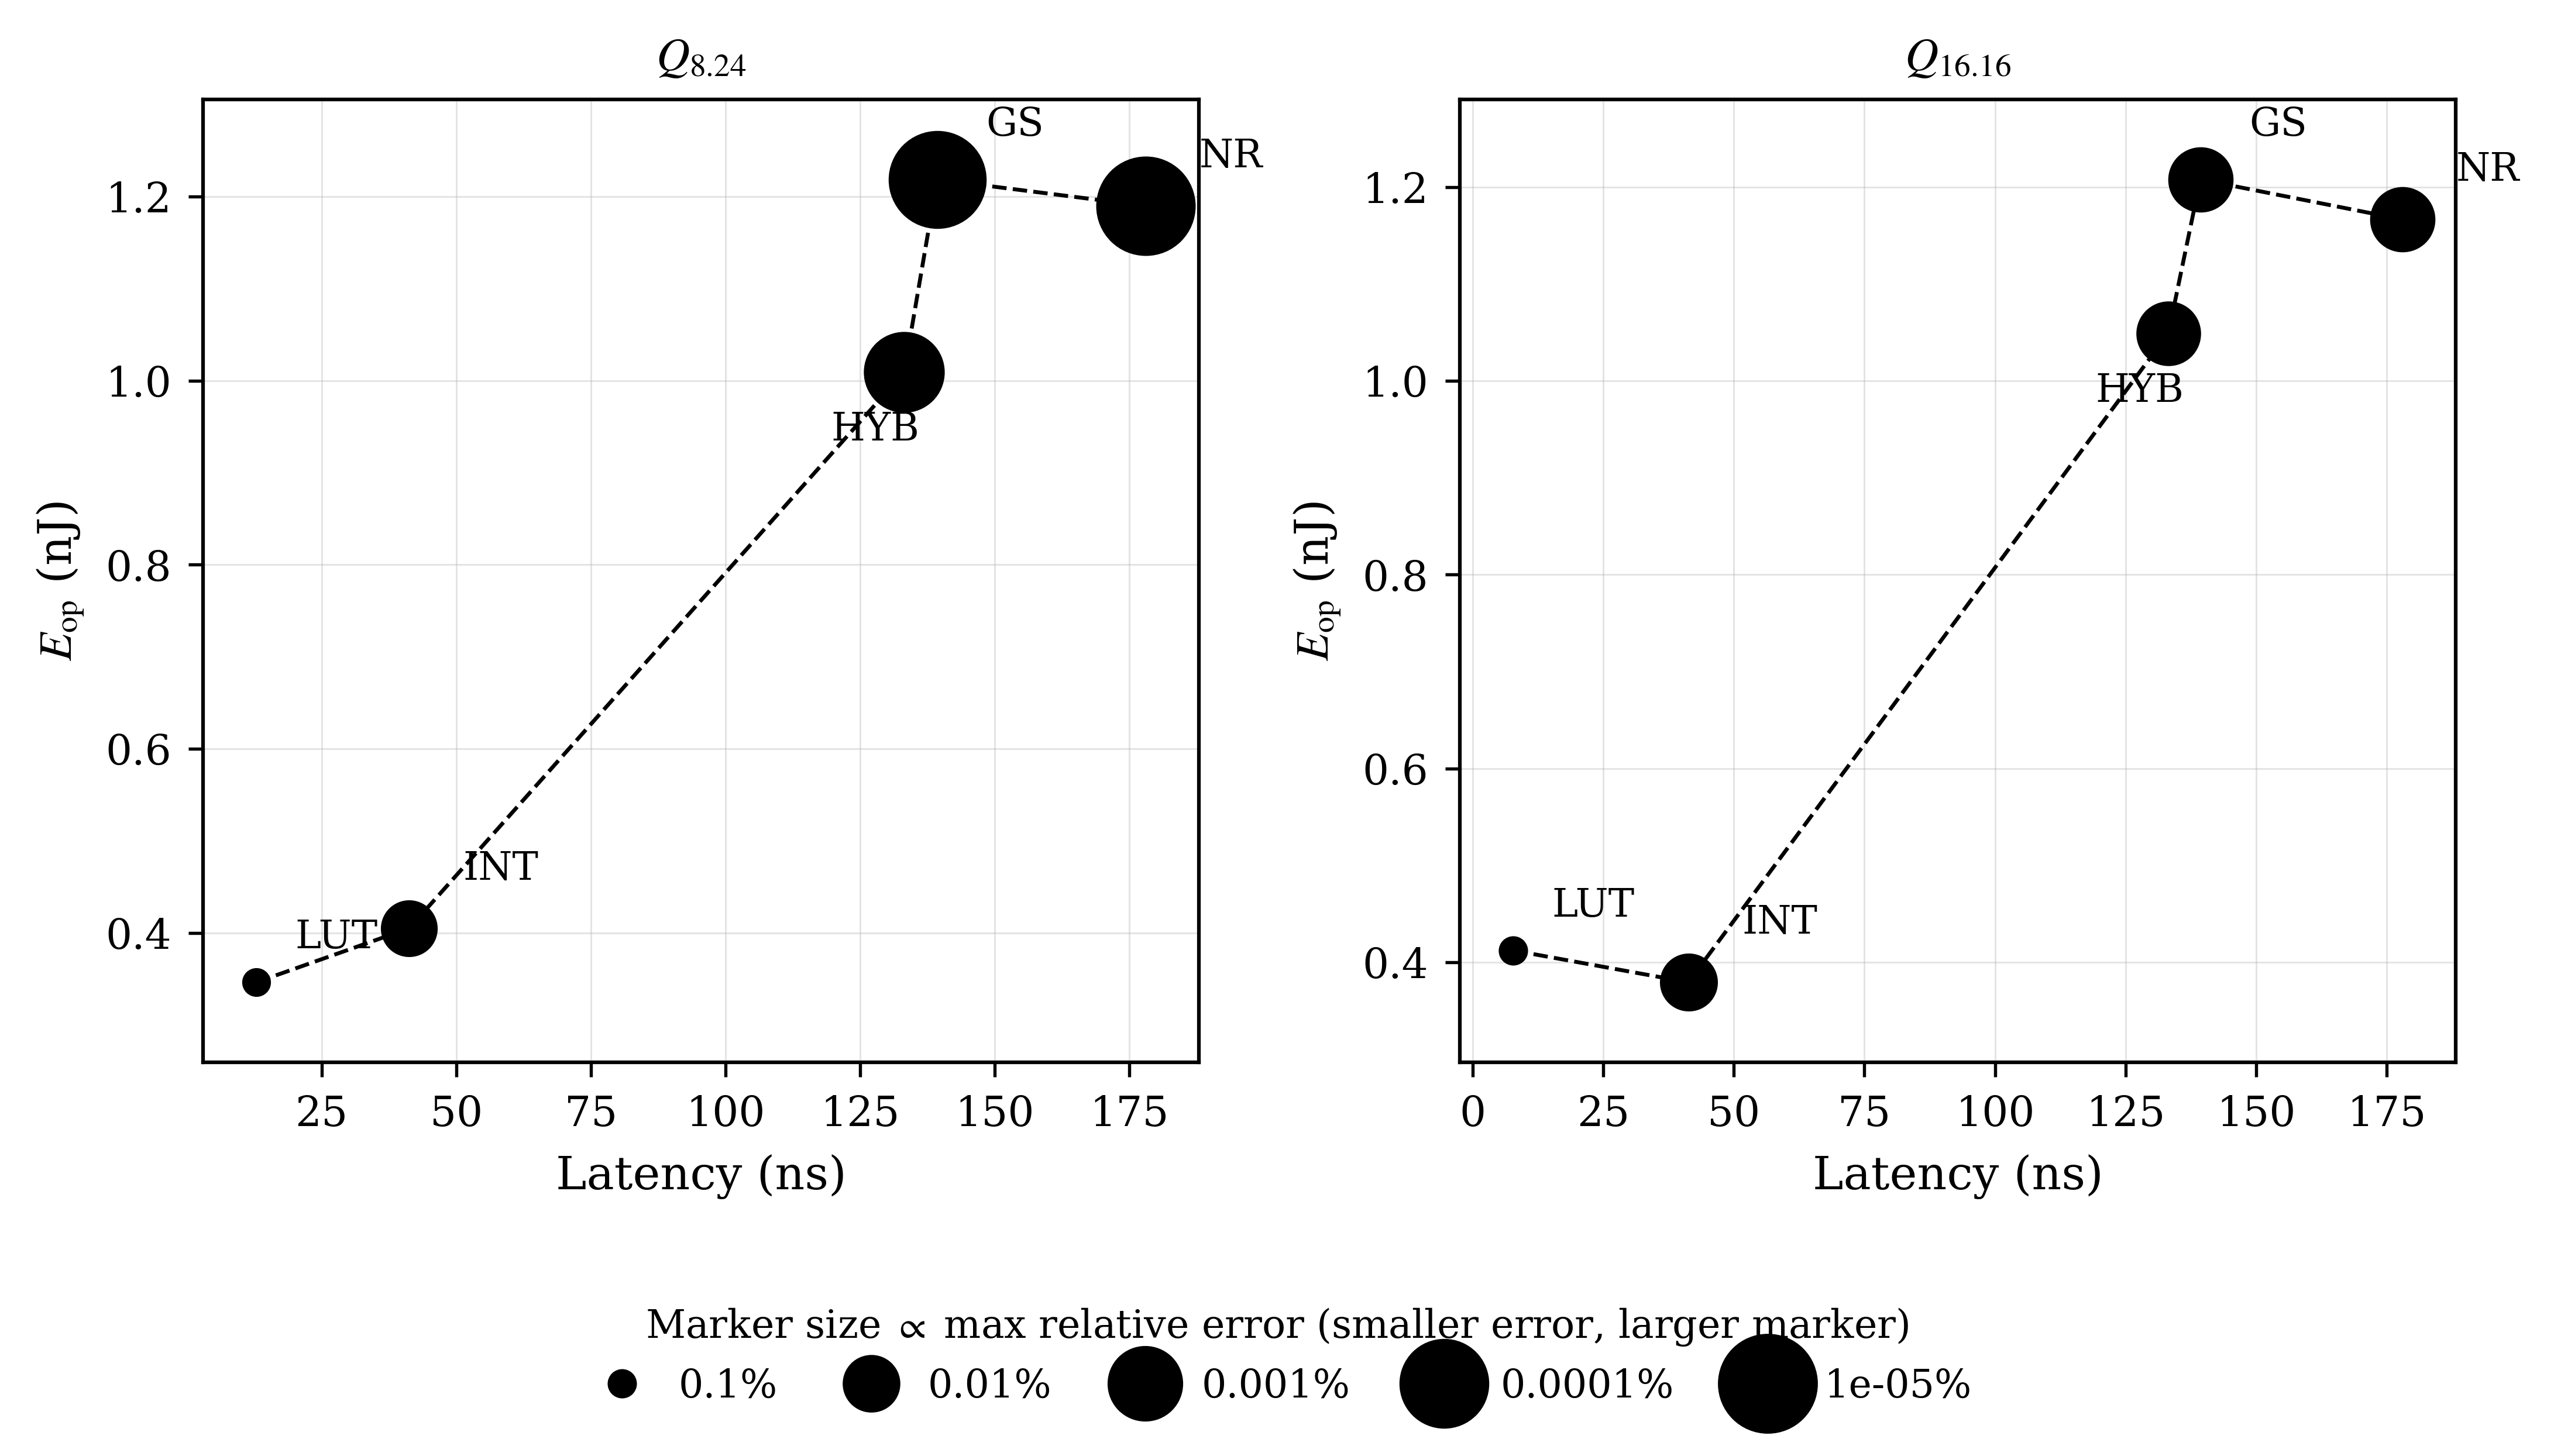
\includegraphics[width=0.9\linewidth]{figures/pareto_front_plot.png}
\caption{Pareto trade-off in the latency--energy plane (latency in ns, energy per operation in nJ/op) by architecture, Q8.24 (left) and Q16.16 (right). Marker size is inversely related to maximum relative error (\%) on a shared global scale across both panels; all five architectures are mutually non-dominated in both formats under strict dominance.}
\Description{Two scatter panels with latency on one axis and energy per operation on the other. In Q8.24, Direct LUT sits at the lowest latency and energy (12.90 ns, 0.346 nJ) and interpolation just above it (41.28 ns, 0.405 nJ). The hybrid lies at 133.32 ns and 1.009 nJ, Goldschmidt at 139.32 ns and 1.219 nJ, and Newton-Raphson at the highest latency and near-highest energy (178.02 ns, 1.190 nJ). In Q16.16 the pattern is similar, with Direct LUT at 7.74 ns and 0.412 nJ and interpolation at 41.28 ns and a lower 0.379 nJ. Marker size is largest for Newton-Raphson and Goldschmidt in Q8.24 and smallest for Direct LUT in both panels.}
\label{fig:paretofront}
\end{figure}

% The radar / Pareto-score figure below is disabled: the paper defines no scalar "Pareto score",
% and the analysis deliberately avoids weighting. Re-enable only after defining and justifying the score.
\begin{figure}[H]
\centering
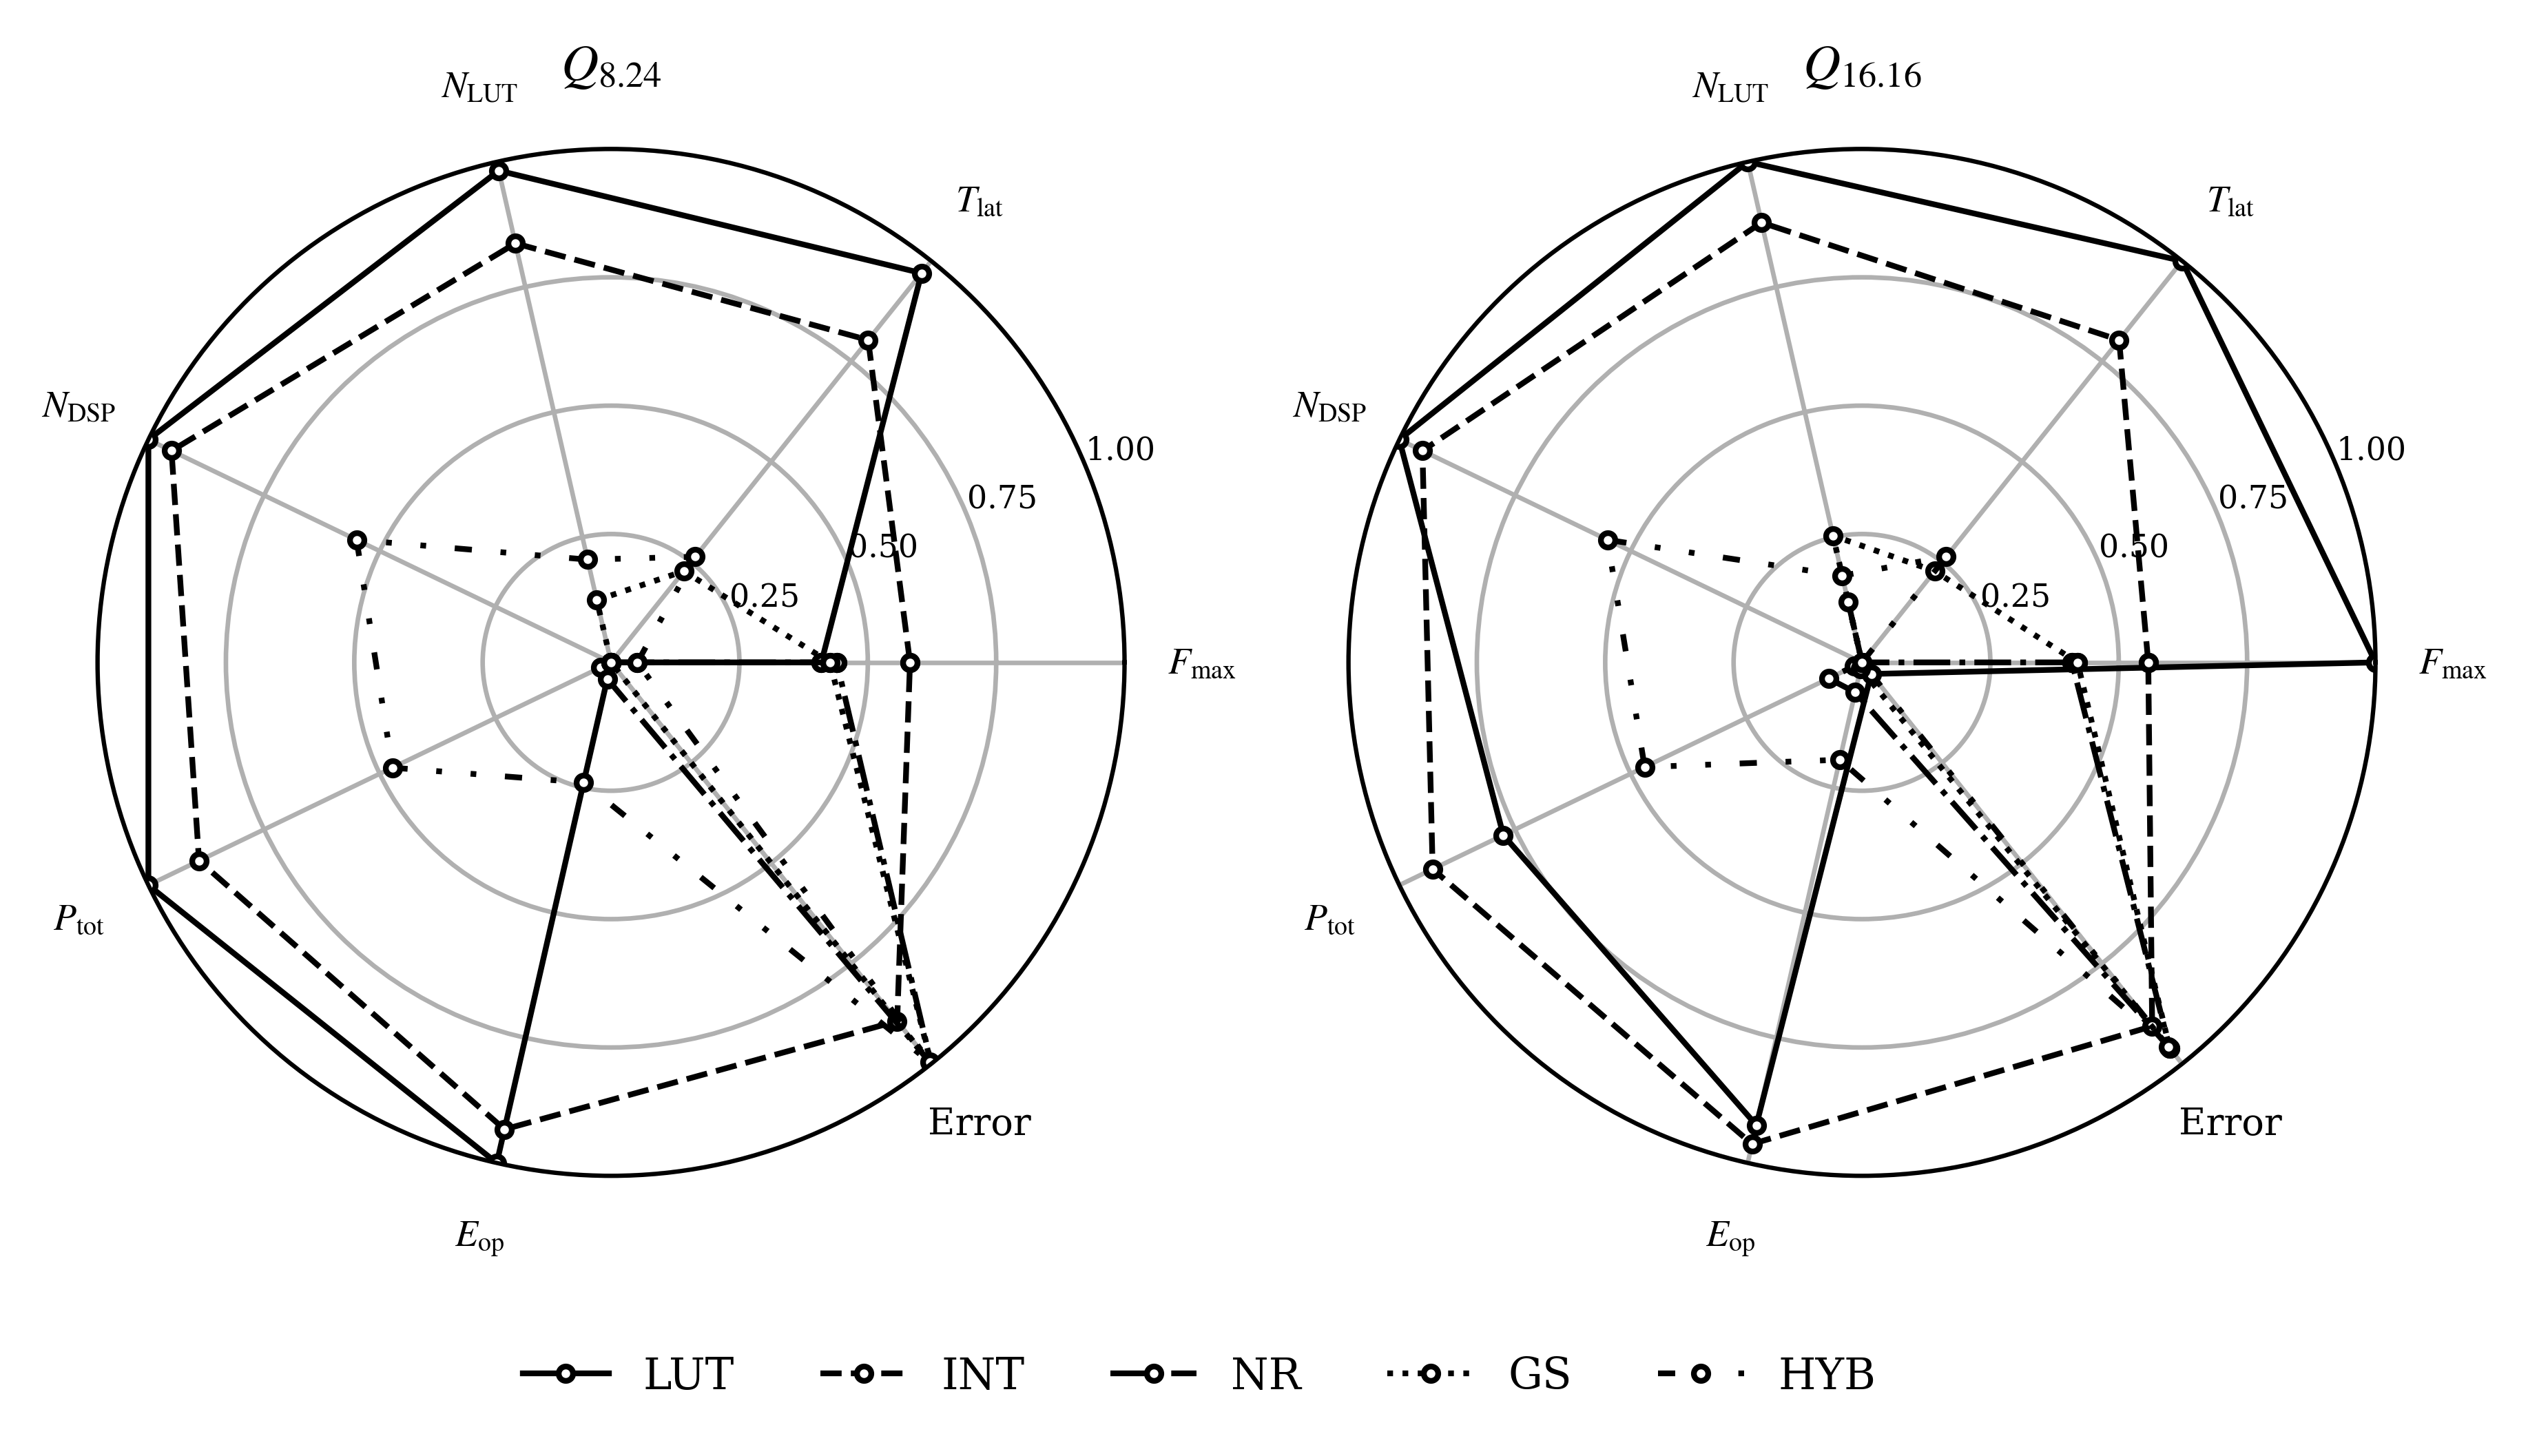
\includegraphics[width=\linewidth]{figures/radar_chart_plot.png}
\caption{Pareto score radar plot for the evaluated architectures.}
\Description{Showcases a multi dimensional pareto tradeoff radar plot for both the q8.24 and q16.16 architectures.}
\label{fig:paretoradar}
\end{figure}
\begin{figure}[H]
\centering
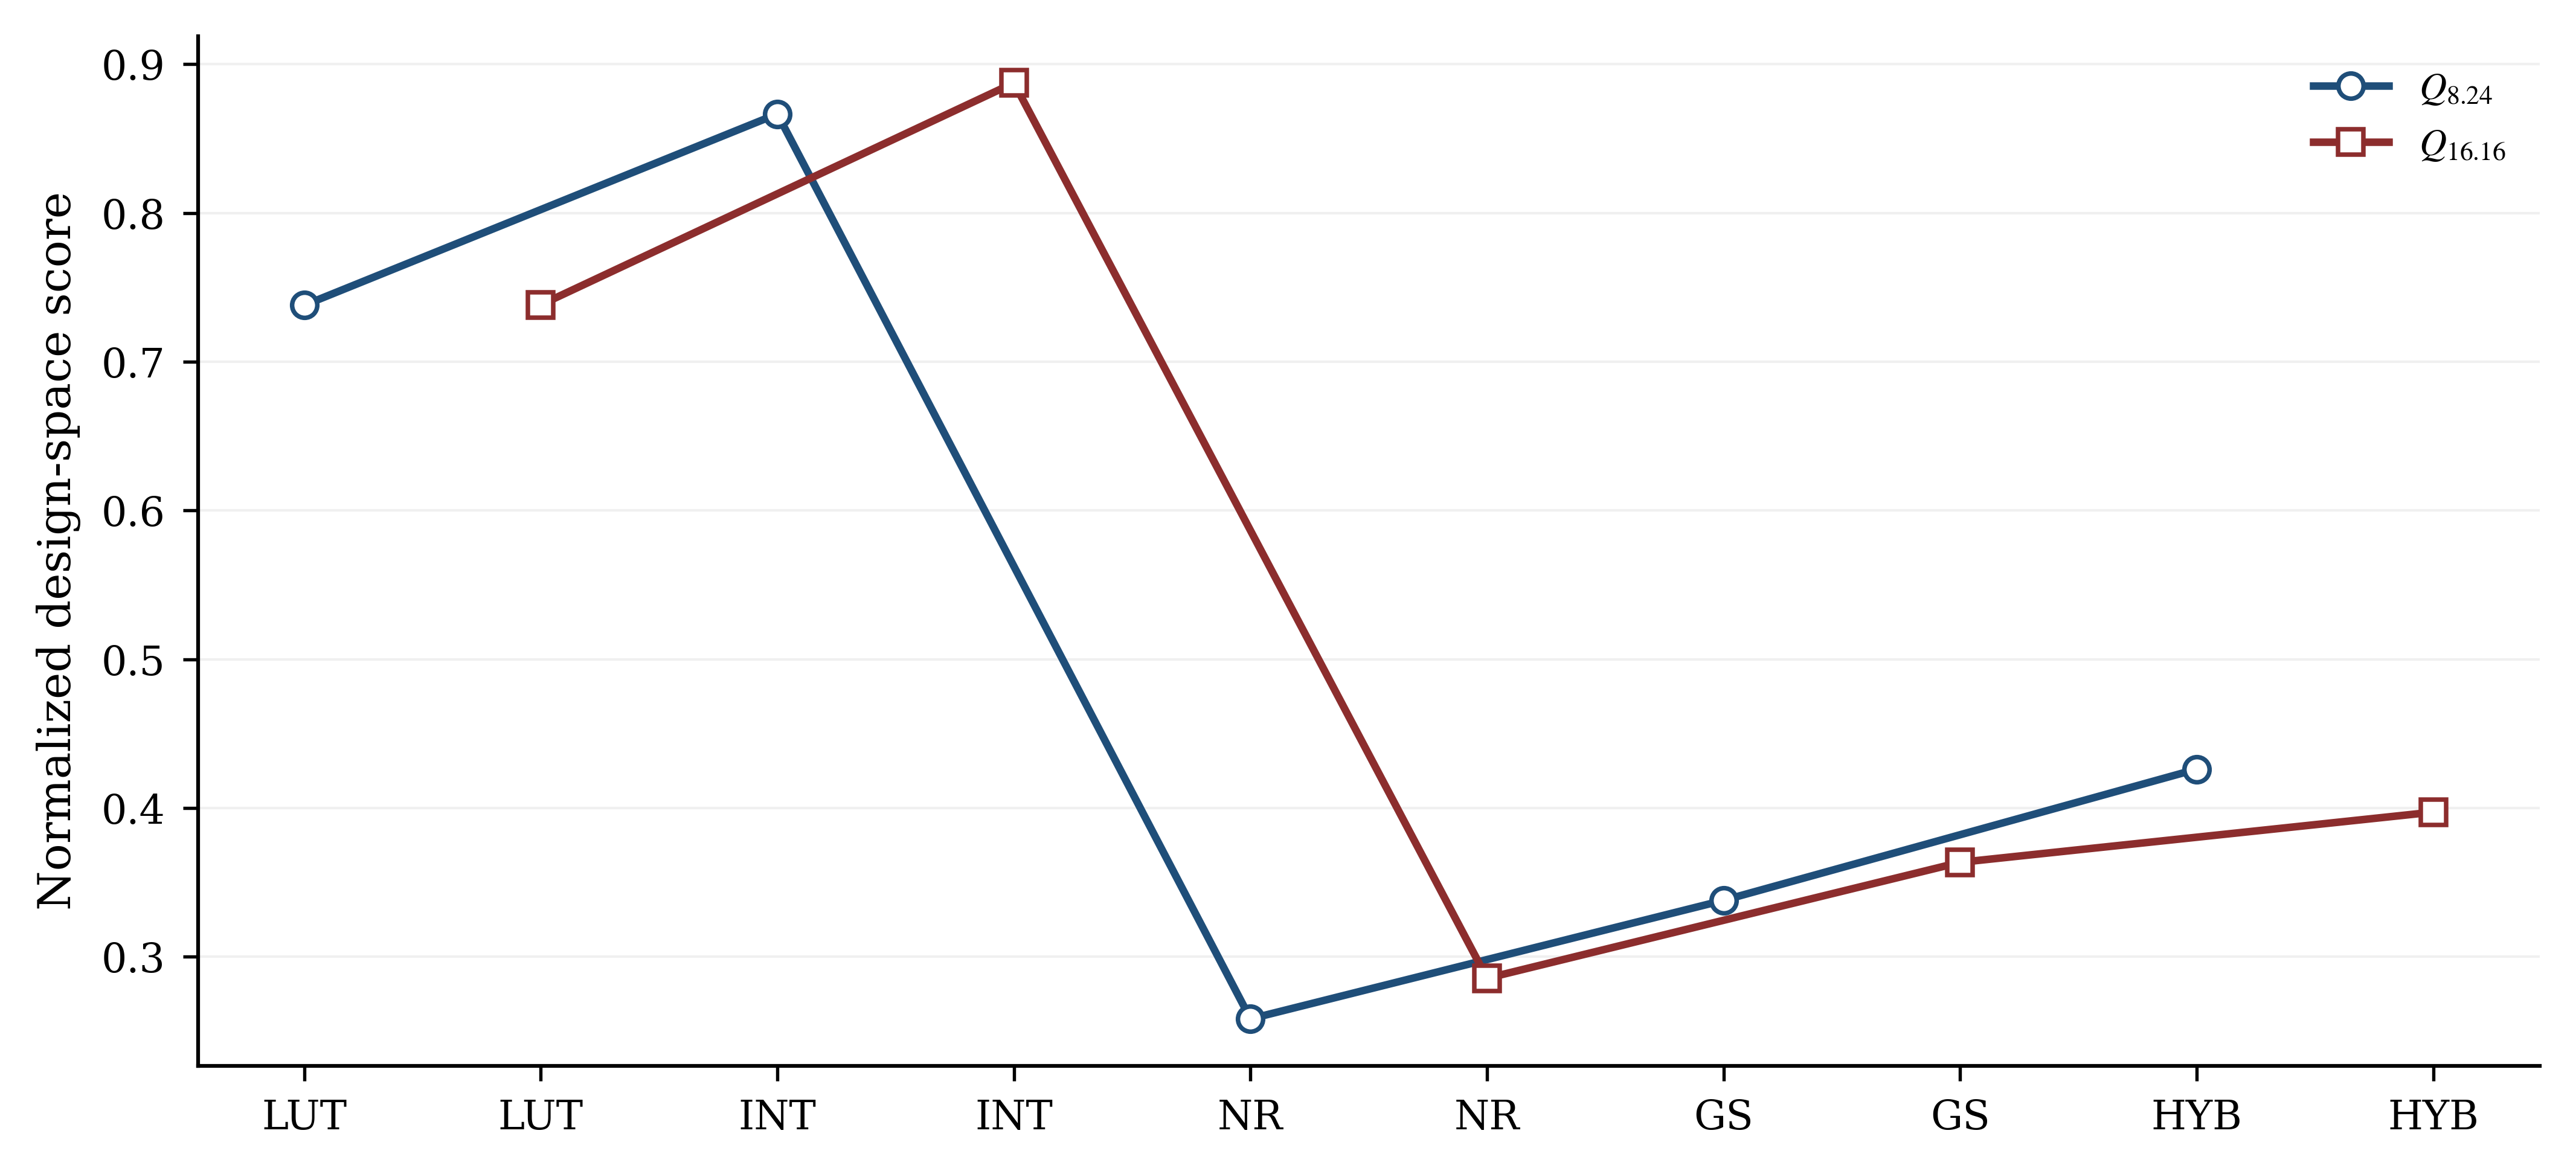
\includegraphics[width=\linewidth]{figures/pareto_score_plot.png}
\caption{Pareto score line plot for the evaluated architectures.}
\Description{Pareto score line plot showing normalized Pareto scores for the evaluated architectures.}
\label{fig:pareto_comparison}
\end{figure}


\subsection{Trade-off Analysis}

Within the Q8.24 non-dominated set, Direct LUT occupies the low-latency and low-energy region of the trade-off surface, with a latency of 12.9~ns, energy of 0.346~nJ/op, and maximum relative error of 0.098\%. Newton-Raphson occupies the high-accuracy region, achieving $1.5\times10^{-5}$\% maximum relative error at 178.0~ns latency and 1.190~nJ/op. Goldschmidt provides comparable numerical accuracy, with a maximum relative error of $2.0\times10^{-5}$\%, while reducing latency by approximately 22\% to 139.3~ns. This latency reduction is accompanied by a small increase in energy per operation, from 1.190 to 1.219~nJ/op (approximately 2.4\%). Thus, the measured Goldschmidt implementation represents a lower-latency alternative to Newton-Raphson when latency is prioritized over a small difference in energy per operation.

The Hybrid architecture occupies an intermediate region of the trade-off surface. It achieves 133.32~ns latency and 1.009~nJ/op, both lower than the corresponding values of the full iterative architectures, while achieving a maximum relative error of $4.09\times10^{-4}$\%. This represents more than an order-of-magnitude improvement over interpolation-only accuracy ($1.04\times10^{-2}$\%). The result demonstrates the distinct trade-off obtained by combining a 9-bit-address interpolated seed with a single Newton-Raphson refinement, providing an intermediate accuracy, latency, energy, and DSP-utilization point between table-based and fully iterative approaches. This intermediate accuracy positioning is specific to Q8.24; in Q16.16 the hybrid error is within about 8\% of the iterative architectures, as discussed above.

\subsection{Energy-Delay Product}
\label{sec:edp}

Table~\ref{tab:edp} reports energy-delay product (EDP $= E_{op} \times L_{ns}$) for all ten architecture/format combinations as a secondary combined figure of merit illustrating the interaction between energy and latency, per the reasoning in Section~\ref{sec:paretoform}. EDP reproduces the same broad ranking as the individual latency and energy metrics, with Direct LUT lowest and the full iterative architectures highest. It is a derived metric rather than a universal physical objective, and the three-objective Pareto analysis above remains the primary basis for comparison.

\begin{table}[H]
\caption{Energy-Delay Product (EDP = Energy/op $\times$ Latency)}
\label{tab:edp}
\begin{tabular}{@{}llrr@{}}
\toprule
\textbf{Architecture} & \textbf{Format} & \textbf{Energy/op (nJ)} & \textbf{EDP (nJ$\cdot$ns)} \\
\midrule
Direct LUT & Q8.24 & 0.346 & 4.46 \\
Direct LUT & Q16.16 & 0.412 & 3.19 \\
LUT-Interpolation & Q8.24 & 0.405 & 16.72 \\
LUT-Interpolation & Q16.16 & 0.379 & 15.66 \\
Newton-Raphson & Q8.24 & 1.190 & 211.80 \\
Newton-Raphson & Q16.16 & 1.167 & 207.68 \\
Goldschmidt & Q8.24 & 1.219 & 169.79 \\
Goldschmidt & Q16.16 & 1.208 & 168.24 \\
Hybrid & Q8.24 & 1.009 & 134.56 \\
Hybrid & Q16.16 & 1.049 & 139.85 \\
\bottomrule
\end{tabular}
\end{table}

\subsection{Consolidated Summary of Results}
\label{sec:consolidated}

Table~\ref{tab:consolidated} consolidates the key metrics from Tables~\ref{tab:resources}-\ref{tab:power} and Table~\ref{tab:edp} into a single reference table, for readers who want the complete set of headline figures for all ten architecture/format combinations without cross-referencing multiple tables.

\begin{table}[H]
\small
\setlength{\tabcolsep}{3pt}
\caption{Consolidated Summary of All Reported Metrics, All Architectures and Formats}
\label{tab:consolidated}
\begin{tabular}{@{}llrrrrrrr@{}}
\toprule
\textbf{Architecture} & \textbf{Format} & \textbf{Slice LUT\%} & \textbf{DSP} & \textbf{Latency (ns)} & \textbf{Max Rel. Err (\%)} & \textbf{Total P (W)} & \textbf{Energy/op (nJ)} & \textbf{EDP (nJ$\cdot$ns)} \\
\midrule
Direct LUT & Q8.24 & 0.03\% & 0 & 12.90 & 0.097596 & 0.136 & 0.346 & 4.46 \\
Direct LUT & Q16.16 & 0.003\% & 0 & 7.74 & 0.094787 & 0.214 & 0.412 & 3.19 \\
LUT-Interpolation & Q8.24 & 0.25\% & 1 & 41.28 & 0.010396 & 0.174 & 0.405 & 16.72 \\
LUT-Interpolation & Q16.16 & 0.19\% & 1 & 41.28 & 0.009156 & 0.161 & 0.379 & 15.66 \\
Newton-Raphson & Q8.24 & 1.52\% & 20 & 178.02 & 0.000015 & 0.475 & 1.190 & 211.80 \\
Newton-Raphson & Q16.16 & 1.34\% & 20 & 178.02 & 0.003815 & 0.458 & 1.167 & 207.68 \\
Goldschmidt & Q8.24 & 1.33\% & 20 & 139.32 & 0.000020 & 0.483 & 1.219 & 169.79 \\
Goldschmidt & Q16.16 & 1.14\% & 20 & 139.32 & 0.003814 & 0.477 & 1.208 & 168.24 \\
Hybrid & Q8.24 & 1.21\% & 9 & 133.32 & 0.000409 & 0.319 & 1.009 & 134.56 \\
Hybrid & Q16.16 & 1.26\% & 9 & 133.32 & 0.004118 & 0.320 & 1.049 & 139.85 \\
\bottomrule
\end{tabular}
\end{table}

\section{Discussion}
\label{sec:discussion}

\subsection{Architecture-Level Trade-offs}

The results of Sections~\ref{sec:results} and~\ref{sec:pareto} illustrate several distinct architecture-level trade-offs. For applications in which latency and energy are important constraints and an error on the order of \textbf{0.1\%} is acceptable, the \textbf{Direct LUT} architecture provides the shortest pipeline and negligible logic utilization, while requiring one of the largest BRAM footprints among the evaluated designs. For the \textbf{Q8.24} results, applications requiring maximum relative error below approximately $\mathbf{10^{-4}}$\% are served by the full iterative architectures, which provide substantially higher numerical accuracy than the table-based approaches. Within this accuracy range, the latency advantage of \textbf{Goldschmidt} over Newton-Raphson (Section~\ref{sec:pareto}) is accompanied by an energy-per-operation increase of approximately \textbf{2.4\% in Q8.24 and 3.5\% in Q16.16}. The \textbf{hybrid} architecture provides a distinct intermediate trade-off by combining a 9-bit-address interpolated seed with a single Newton-Raphson refinement. In Q8.24 it achieves substantially lower error than interpolation alone while reducing the hardware cost of full iterative refinement, with approximately \textbf{75\% of the Newton-Raphson latency and 45\% of the DSP utilization of either full iterative architecture}. In Q16.16, where the iterative and hybrid errors are within about 8\% of one another, the Hybrid architecture offers similar accuracy with lower latency, energy, and DSP usage.

\subsection{Applicability}

The reciprocal approximation architectures evaluated in this work are applicable wherever a fixed-point, division-free reciprocal is required as a building block within a larger FPGA arithmetic pipeline. Representative applications include normalization stages in adaptive and statistical signal processing, such as computing a z-score or an Ornstein-Uhlenbeck mean-reversion signal, where division by a continuously updated scale or standard-deviation term may be required; coordinate and vector normalization in graphics and radar/sonar signal chains, where a reciprocal can precede a subsequent multiplication; and floating-point division and mantissa-normalization units, where the reciprocal is applied to a range-reduced significand. In these settings, the appropriate architecture depends on the required combination of \textbf{numerical precision, latency, throughput, resource utilization, and energy}, with the evaluated designs occupying different regions of the corresponding trade-off space rather than a single architecture being universally optimal.

\subsection{Limitations}

Several limitations should be considered when interpreting and generalizing the results. First, all experiments use a single input domain, $x \in [0.5, 2.5]$. Although this range represents the bounded reciprocal domain considered in Section~\ref{sec:fixedpoint} and captures the characteristic error concentration near the lower bound discussed in Section~\ref{sec:accuracy}, the evaluation does not include alternative or non-uniform input distributions. Such distributions may alter the observed accuracy and performance trade-offs among the architectures.

Second, the evaluation is limited to a single FPGA family, Xilinx Artix-7. The relative costs of BRAM, DSP, slice LUT, and FF resources are device-dependent; consequently, the specific resource-utilization trade-offs reported in Table~\ref{tab:resources} may differ on other FPGA families or vendor platforms. The timing and power characteristics may likewise change with the underlying device architecture and implementation resources. In addition, the reported power values are post-implementation tool estimates rather than board-level measurements, and the Hybrid architecture was evaluated against a less aggressive clock target than the other four architectures.

Third, the study does not include a direct comparison with vendor-supplied divider or reciprocal IP cores, such as Xilinx LogiCORE-class implementations, nor with CORDIC-based reciprocal/division computation \cite{Volder59,Andraka98}, which trades the multiplier-centric datapaths evaluated here for a shift-and-add rotation structure well suited to FPGA fabrics with limited DSP resources. Such comparisons would provide additional baselines for evaluating the custom architectures against off-the-shelf and multiplier-free solutions and are therefore left for future work.

Finally, the evaluated iterative architectures use fixed iteration configurations: \textbf{two Newton-Raphson iterations, two Goldschmidt iterations, and one Newton-Raphson refinement iteration following LUT interpolation in the Hybrid architecture}. The seed-table sizes and interpolation resolutions are likewise fixed for the evaluated configurations. A broader exploration varying iteration count, seed-table size, and interpolation resolution could expose additional points in the accuracy, latency, resource, and energy trade-off space beyond the five architectures evaluated in this study.

\section{Conclusion}
\label{sec:conclusion}

This work presented a post-implementation comparative evaluation of five fixed-point reciprocal approximation architectures (Direct LUT, LUT with Linear Interpolation, Newton-Raphson, Goldschmidt, and a hybrid LUT-Interpolation/Newton-Raphson architecture) implemented in Q8.24 and Q16.16 fixed-point formats on a Xilinx Artix-7 XC7A100T FPGA. All architectures were evaluated using a common input domain of $x \in [0.5, 2.5]$ and one million verification vectors, enabling accuracy, latency, resource utilization, and energy to be compared under a common evaluation framework with architecture-specific timing constraints.

The results demonstrate substantial differences in the hardware and numerical characteristics of the evaluated architectures. The Direct LUT architecture provides the shortest pipelines, at the cost of the largest table-based memory requirement and the highest approximation error among the evaluated designs. LUT-based linear interpolation substantially reduces approximation error while retaining a relatively shallow pipeline. The two iterative architectures provide substantially higher numerical accuracy but require deeper pipelined datapaths and significantly greater DSP and flip-flop utilization. The Hybrid architecture combines a 9-bit-address interpolated seed with a single Newton-Raphson refinement iteration, providing an intermediate point in the accuracy, latency, DSP, and energy trade-off space.

The comparison also demonstrates that fixed-point format selection has a direct interaction with reciprocal architecture. Q8.24 generally preserves substantially higher numerical accuracy for the iterative and hybrid architectures because of its larger fractional field, whereas Q16.16 reduces fractional precision and consequently increases the observed approximation error for these architectures. At the same time, the change in fractional precision does not produce a uniform hardware advantage across all architectures, illustrating that arithmetic precision, memory organization, pipeline structure, and FPGA resource mapping must be considered together when selecting a fixed-point reciprocal implementation.

Across the evaluated designs, the maximum relative error spans more than three orders of magnitude, while latency spans more than an order of magnitude. Energy per operation varies by approximately $3.5\times$, from 0.346~nJ/op to 1.219~nJ/op. The three-objective Pareto analysis further shows that all five architectures are strictly non-dominated within each fixed-point format: each occupies a distinct point in the accuracy-latency-energy design space rather than being uniformly superseded by another evaluated architecture. In Q16.16, however, this result depends on error differences of at most about 8\% among the iterative and hybrid architectures, so it should be interpreted with that qualification. Reciprocal architecture selection is therefore application-dependent, with the appropriate implementation determined by the required balance among numerical precision, pipeline latency, throughput, energy, and FPGA resource availability.

Overall, the study provides a common evaluation framework for understanding these trade-offs across lookup-based, interpolated, iterative, and hybrid reciprocal architectures. Rather than identifying a universally optimal implementation, the results establish quantitative design points that can be used to select or further optimize a reciprocal architecture according to the constraints of a target FPGA application. Future work can extend this design space to additional FPGA families, alternative input distributions, vendor-supplied reciprocal/division IP, board-level power measurement, and systematic variation of seed-table resolution and iteration count to investigate configurations beyond the five evaluated architectures.

The complete RTL implementations, verification testbenches, datasets, and analysis scripts are publicly available in the accompanying GitHub repository~\cite{GitHubRepo}, enabling reproducibility of the reported results.

%%
%% The acknowledgments section is defined using the "acks" environment
%% (and NOT an unnumbered section). This ensures the proper
%% identification of the section in the article metadata, and the
%% consistent spelling of the heading.
\begin{acks}
Artificial intelligence (AI) tools like Claude and Gemini were used as research-assistance tools during the development and documentation of this work. The assistance included SystemVerilog debugging, examination of fixed-point arithmetic and pipeline behavior, identification of potential RTL implementation issues, creation of block diagrams (Figures 1 to 5), and limited refinement of technical writing. AI-generated suggestions were treated as candidate solutions and were not accepted without verification. Proposed RTL modifications were validated through compilation and cycle-accurate simulation, while hardware-related changes were subsequently evaluated through FPGA synthesis and implementation. Numerical-analysis procedures were cross-checked against independently computed reference values and the common verification dataset described in this work. AI tools were not used to generate, fabricate, or alter experimental measurements. The reported FPGA resource utilization, timing, latency, power, energy, and numerical-accuracy results were obtained from the corresponding simulation and FPGA implementation workflows. 
\end{acks}

\bibliographystyle{ACM-Reference-Format}
\bibliography{references}

\end{document}